%%% Document Options %%%
% Compile with XeLaTeX (or LuaLaTeX) + Biber, with shell escape enabled (needed by minted).
% On Overleaf: Menu -> Compiler -> XeLaTeX. Main document: main.tex.
\documentclass[
    school=iith,
    language=english,
    chapterstyle=classic,
    coverstyle=classic
]{IITHThesis}

%%% Extra packages used by this report %%%
\usepackage{amsthm}
\usepackage{tikz}
\usetikzlibrary{arrows.meta, positioning, fit, calc, shapes.geometric, backgrounds}
\usepackage{algorithm}
\usepackage{algpseudocode}
\usepackage{pifont}
\usepackage{placeins} % \FloatBarrier keeps result figures out of the Limitations section

%%% Number subsubsections (used for the result sections) %%%
\setcounter{secnumdepth}{3}

%%% Paragraph spacing (chapters use \parindent0pt) %%%
\setlength{\parskip}{5pt plus 1pt minus 1pt}

%%% Theorem-like environments %%%
\theoremstyle{plain}
\newtheorem{proposition}{Proposition}[chapter]
\newtheorem{lemma}[proposition]{Lemma}
\newtheorem{corollary}[proposition]{Corollary}
\theoremstyle{definition}
\newtheorem{definition}[proposition]{Definition}
\newtheorem{assumption}{Assumption}
\renewcommand{\theassumption}{A\arabic{assumption}}
\theoremstyle{remark}
\newtheorem{remark}[proposition]{Remark}

%%% Report-specific colours, boxes and macros %%%
\definecolor{naivecol}{HTML}{C53030}
\definecolor{gatedcol}{HTML}{2B6CB0}
\definecolor{oraclecol}{HTML}{2F855A}
\definecolor{boxblue}{HTML}{0D47A1}
\definecolor{boxbg}{HTML}{EEF4FB}

\newtcolorbox{keybox}[1][Key idea]{
    enhanced, unbreakable, % short boxes: never split across pages
    colback=boxbg, colframe=boxblue,
    boxrule=0.6pt, arc=2pt, left=6pt, right=6pt, top=4pt, bottom=4pt,
    fonttitle=\bfseries\small, coltitle=white, title={#1}
}
\newtcolorbox{findingbox}[1][Finding]{
    enhanced, unbreakable, % short boxes: never split across pages
    colback=green!3!white, colframe=green!40!black,
    boxrule=0.6pt, arc=2pt, left=6pt, right=6pt, top=4pt, bottom=4pt,
    fonttitle=\bfseries\small, coltitle=white, title={#1}
}

\newcommand{\naive}{\textcolor{naivecol}{\textbf{naive}}}
\newcommand{\gated}{\textcolor{gatedcol}{\textbf{gated}}}
\newcommand{\tcode}[1]{\texttt{\small #1}}
\newcommand{\Kn}{\mathsf{K}}
\newcommand{\Bl}{\mathsf{B}}
\newcommand{\Hyp}{\mathcal{H}}
\newcommand{\cmark}{\textcolor{green!50!black}{\ding{51}}}
\newcommand{\xmark}{\textcolor{naivecol}{\ding{55}}}
\newcommand{\repolink}{\url{https://github.com/spamprx/Aerial_Simulator}}

%%% Document Metadata %%%
% Title (Mandatory)
\Title{VeriFly: Verified Search and Rescue with an Untrusted UAV Fleet}

% Subtitle (Mandatory)
\Subtitle{
\textbf{Group Design Project Report} \\
\vspace{0.1in}
\textbf{Team Name:} Aerial \\
\vspace{0.05in}
{\normalsize Resilient 3D Aerial Traffic Management and Knowledge-Gated Coordination for UAV Fleets in Disaster Response}
}

% University (Mandatory)
\University{IIT Hyderabad}

\Course{AI3403 - Multi-Agent Systems}

% Department (Mandatory)
\Department{Department of Artificial Intelligence}

% Institution (Mandatory)
\Institution{Indian Institute of Technology Hyderabad}

% Thesis Theme (Mandatory)
\ThesisType{GDP: IITH-AI-MAS-2026-\#0001}

% Local & Date (Mandatory)
\Date{Kandi, Telangana, INDIA - \DTMmonthname{\month} \number\year}

% Academic Year
\AcademicYear{2026/27}


%%% Loading of Glossary and Acronyms %%%
\makeglossaries
\loadglsentries{Matter/04-Glossary}
\loadglsentries[\acronymtype]{Matter/05-Acronyms}

\begin{document}

%%% Front Matter %%%
\ifthenelse{\equal{\CoverOption}{classic}}{
    \newcommand\BackgroundPicCover{%
    \put(0,0){%
    \parbox[b][\paperheight]{\paperwidth}{%
    \vfill
    \centering
    
\includegraphics[width=\paperwidth,height=\paperheight,keepaspectratio]{Figures/Theme/Cover-BG.pdf}%
    \vfill
    }}}
}{
    \newcommand\BackgroundPicCover{%
    \put(0,0){%
    \parbox[b][\paperheight]{\paperwidth}{%
    \vfill
    \centering
    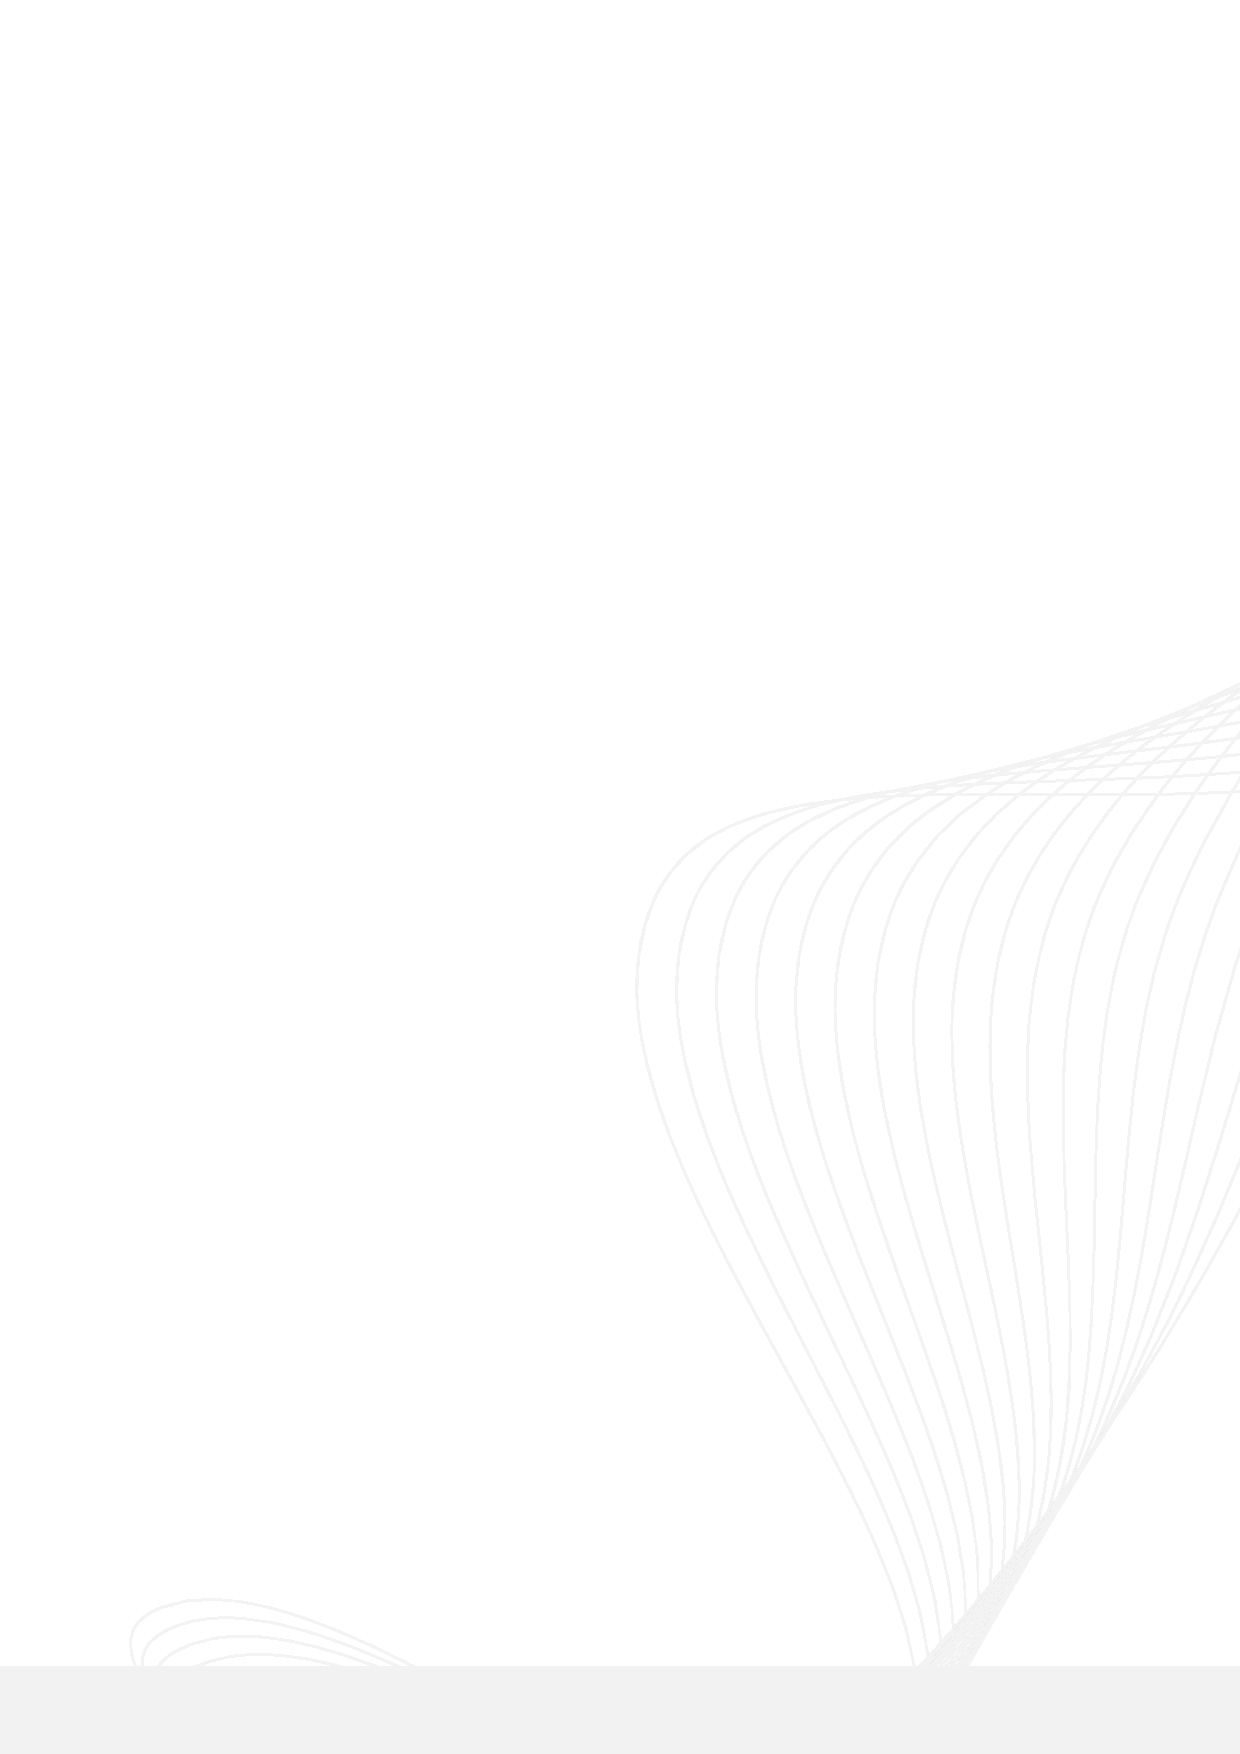
\includegraphics[width=\paperwidth,height=\paperheight,keepaspectratio]{Figures/Theme/Front-Page-BG.pdf}%
    \vfill
    }}}
} 

\AddToShipoutPictureBG*{\BackgroundPicCover}

\newgeometry{margin=1.98cm, top=2.15cm, bottom=1.47cm}
\begin{titlepage}
    %\latofont
    \ifthenelse{\equal{\CoverOption}{classic}}{\color{white}}{\color{frontpagedark}}
    \vspace*{\baselineskip}

    \vspace{4.5\baselineskip}

    % Logo.
    \begin{textblock*}{5cm}(-1.0cm,-5.0cm) % {block width} (coords)
    
\includegraphics[scale=0.40]{Figures/IITH LogoHorizontal.png}
    \end{textblock*}

    \vspace{50pt}

    
	\noindent
    \makebox[\textwidth][l]{%
        \parbox{\dimexpr\textwidth-3cm\relax}{
            \setstretch{1.03}
            \raggedright\bfseries\fontsize{25}{25}\selectfont\GetTitle
        }
    }

    \vspace{35pt}

    \vspace{0.8\baselineskip}

    % Subtitle.
    \noindent
    \makebox[\textwidth][l]{%
        \parbox{\dimexpr\textwidth-2cm\relax}{
            \setstretch{1.03}
            \raggedright\fontsize{18}{18}\selectfont\GetSubtitle
        }
    }

    \vspace{35pt}  

    % Author.
    {\noindent \Large \textbf{Team Members:} 
    \begin{enumerate}
        \item \fontsize{14}{19}\selectfont Rithvik Jami (Team Leader) \quad {\normalsize (CS23BTECH11022)}
        \item \fontsize{14}{19}\selectfont Praneeth Chamarthy \quad {\normalsize (CS23BTECH11012)}
        \item \fontsize{14}{19}\selectfont Muvvala Sai Ram Suhas \quad {\normalsize (CS23BTECH11038)}
        \item \fontsize{14}{19}\selectfont Jakkala Naga Rohith Kumar \quad {\normalsize (CS23BTECH11021)}
        \item \fontsize{14}{19}\selectfont Gona Sanjana \quad {\normalsize (CS23BTECH11019)}
        \item \fontsize{14}{19}\selectfont Prabhu Teja \quad {\normalsize (CS23BTECH11050)}
    \end{enumerate}
    }
    

    \vspace{20pt}
 
	\vfill

    {
    \Large

    % Course.
    {\noindent\GetCourse}
    
    % Department.
	{\noindent\GetDepartment}

    % Degree.
	{\noindent\GetInstitution}    

    \vspace{35pt}

    % Local & Date.
	{\noindent\GetDate}
    }

    \vspace{28pt}
\end{titlepage}
\restoregeometry
\blankpage
\newcommand\BackgroundPicFrontPage{%
    \put(0,0){%
    \parbox[b][\paperheight]{\paperwidth}{%
    \vfill
    \centering
    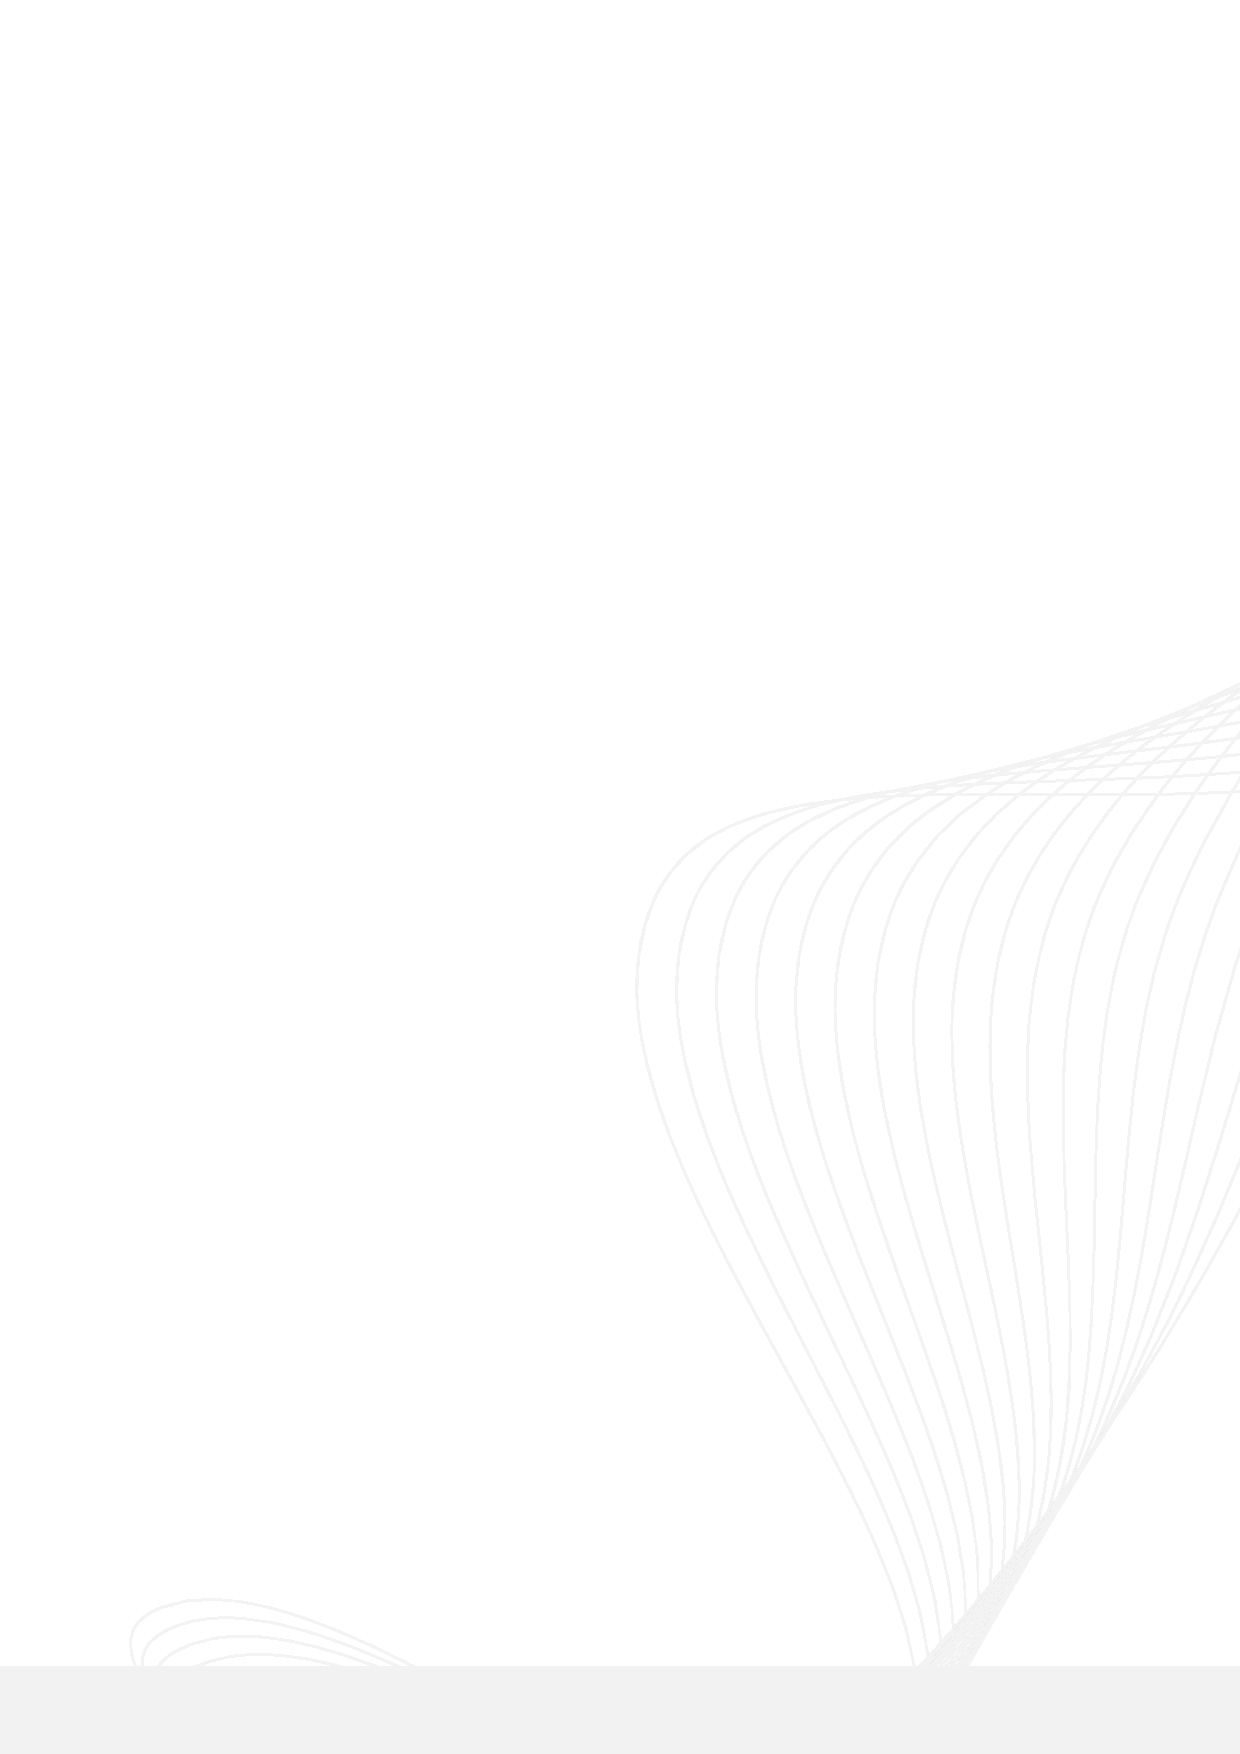
\includegraphics[width=\paperwidth,height=\paperheight,keepaspectratio]{Figures/Theme/Front-Page-BG.pdf}%
    \vfill
}}}
\AddToShipoutPictureBG*{\BackgroundPicFrontPage}

\newgeometry{margin=1.98cm, top=2.15cm, bottom=1.47cm}
\begin{titlepage}
    %\latofont
    \color{frontpagedark}
    \vspace*{\baselineskip}

    % \ifthenelse{\equal{\SchoolOption}{estg}}{
    %     \begin{figure}
    %         \includegraphics[width=0.485\linewidth]{Figures/Theme/Logotypes/IPLeiria-ESTG-Logo-B.pdf}
    %     \end{figure}
    % }

    % \ifthenelse{\equal{\SchoolOption}{cranfield}}{
    %     \begin{figure}
    %         \includegraphics[width=0.3\linewidth]{Figures/Theme/Logotypes/Cranfield_Logo.png}
    %     \end{figure}
    % }
    
    % \ifthenelse{\equal{\SchoolOption}{esad}}{
    %     \begin{figure}
    %         \includegraphics[width=0.485\linewidth]{Figures/Theme/Logotypes/IPLeiria-ESAD-Logo-B.pdf}
    %     \end{figure}
    % }
    
    % \ifthenelse{\equal{\SchoolOption}{esslei}}{
    %     \begin{figure}
    %         \includegraphics[width=0.485\linewidth]{Figures/Theme/Logotypes/IPLeiria-ESSLEI-Logo-B.pdf}
    %     \end{figure}
    % }
    
    % \ifthenelse{\equal{\SchoolOption}{estm}}{
    %     \begin{figure}
    %         \includegraphics[width=0.485\linewidth]{Figures/Theme/Logotypes/IPLeiria-ESTM-Logo-B.pdf}
    %     \end{figure}
    % }
    
    % \ifthenelse{\equal{\SchoolOption}{esecs}}{
    %     \begin{figure}
    %         \includegraphics[width=0.485\linewidth]{Figures/Theme/Logotypes/IPLeiria-ESECS-Logo-B.pdf}
    %     \end{figure}
    % }

    \vspace{3.0\baselineskip}

    % Title.
	\noindent
    \makebox[\textwidth][l]{%
        \parbox{\dimexpr\textwidth-2.5cm\relax}{
            \setstretch{1.03}
            \raggedright\bfseries\fontsize{20}{26}\selectfont\GetTitle
        }
    }

    \vspace{0.8\baselineskip}

    % Subtitle.
    \noindent
    \makebox[\textwidth][l]{%
        \parbox{\dimexpr\textwidth-5cm\relax}{
            \setstretch{1.03}
            \raggedright\fontsize{14}{19}\selectfont\GetSubtitle
        }
    }

    \vspace{25pt}

    % Author.
    {\noindent\bfseries\fontsize{30}{30} {\large Team Members}:
    \begin{enumerate}
        \item \fontsize{14}{19}\selectfont Rithvik Jami (Team Leader) \quad {\normalsize (CS23BTECH11022)}
        \item \fontsize{14}{19}\selectfont Praneeth Chamarthy \quad {\normalsize (CS23BTECH11012)}
        \item \fontsize{14}{19}\selectfont Muvvala Sai Ram Suhas \quad {\normalsize (CS23BTECH11038)}
        \item \fontsize{14}{19}\selectfont Jakkala Naga Rohith Kumar \quad {\normalsize (CS23BTECH11021)}
        \item \fontsize{14}{19}\selectfont Gona Sanjana \quad {\normalsize (CS23BTECH11019)}
        \item \fontsize{14}{19}\selectfont Prabhu Teja \quad {\normalsize (CS23BTECH11050)}
    \end{enumerate}
    }

    \vspace{30pt}    

    {
    \noindent
    \fontsize{10}{12}\selectfont
    \renewcommand{\arraystretch}{0.1}
    \hspace*{-2.5pt}\begin{tabular}{@{}r@{\hspace{5pt}}>{\raggedright\arraybackslash}m{6cm}@{}}

        \textbf{Project Supervisor:} & Dr. Venkatraman Renganathan \\ [-.7ex]
        & \setstretch{0.9}{\fontsize{8}{10}\selectfont\itshape Assistant Professor, IITH} \\ [2ex]      
        
    \end{tabular}
    }
    
    \vfill

    \vspace{15pt}

    % Course.
    {\noindent\fontsize{10}{12}\selectfont\GetCourse}
	
    % Department.
	{\noindent\fontsize{10}{12}\selectfont\GetDepartment}

    % Degree.
	{\noindent\fontsize{10}{12}\selectfont\GetInstitution}
	

    \vspace{35pt}

    % Thesis option.
	{\noindent\fontsize{10}{12}\selectfont\GetThesisType}

    \vspace{35pt}

    % Local and date.
	{\noindent\fontsize{10}{12}\selectfont\GetDate}

    \vspace{38pt}
\end{titlepage}
\restoregeometry

%%% Copyright Statement %%%
\pagenumbering{gobble} % Prevent page numbering.

\vspace*{\fill}

\ifthenelse{\equal{\LanguageOption}{portuguese}}{%
    \noindent \textbf{\GetTitle}
    
    \noindent Copyright \textcopyright~\the\year{} - \GetFirstAuthor, \GetSchool.
    
    \vspace{.575em}
    
    \noindent A presente dissertação é um trabalho original, elaborado exclusivamente para este fim, tendo sido devidamente citados todos os autores cujos estudos contribuíram para a sua elaboração. É permitida a sua reprodução parcial com indicação do autor e referência ao grau, ano letivo, instituição - \textit{Politécnico de Leiria} - e data da defesa pública.
}
{%
\begin{center}
    
\includegraphics[scale=0.40]{Figures/Theme/Logotypes/IITH_Logo.png}
\end{center}

\vspace{100pt}

    \begin{center}
    {\Large
    \textbf{Team Name: Aerial}    \\
    \fontsize{10}{12}\selectfont\GetThesisType \\
    Copyright \textcopyright~\the\year{} \\ 
    \GetUniversity.
    }
    \end{center}
    \vspace{.575em}
    
}

\vspace*{\fill}

\plainblankpage

%%% Roman Numeration %%%
\pagenumbering{roman}

%%% Abstract %%%
\pdfbookmark[1]{Abstract}{abstract}
\chapter*{Abstract}
\thispagestyle{plain}

After an earthquake, a fleet of drones must search a collapsed and \emph{unmapped} city district for survivors with no
control tower: each drone sees only through a narrow camera and talks only to neighbours within a short, lossy radio
range. We study what happens when one or two of these drones are \emph{liars}: they broadcast fake positions,
declare areas ``searched, nobody here'' without searching them, and hide the survivors they see. Our thesis is that
\emph{the filtering that makes a fleet resilient also makes it ignorant}. Resilient consensus (W-MSR) protects the
\emph{numbers} a fleet averages, but a careful liar stays inside the honest range, and a claim such as ``I searched this
block'' is not a number at all.

We built \textbf{VeriFly}, a decentralised 3D simulator with 2.5D terrain, ray-cast cameras, a lossy disk-graph radio
with gossip relaying, and four fleets that run the \emph{same} drone code and differ only in what they trust. The
\gated{} fleet separates \emph{knowing} from \emph{believing}. Every drone keeps an S5 possible-worlds model of who might
be lying. It eliminates worlds with five proof rules that an honest drone can never trigger: UWB range, speed, radio
horizon, camera and audit. It records who vouched for every claim, so a liar's claims are reverted and re-swept
automatically, and it moves only when it \emph{knows} the next manoeuvre is safe ($\Kn_i\,\mathit{Safe}$).

Across 280 paired runs that vary the fleet size, the number of liars and the city size, the gated fleet found
\textbf{100\% of survivors in all 140 runs}, against 82--87\% for the W-MSR-only (\naive{}) fleet with one liar and
\textbf{56\%} with two. The liar was identified in every gated run, typically within a few seconds of starting to lie,
with \textbf{zero false accusations in every server run}. The price of caution is time, about $+90$\,s at the baseline. With a shared
predictive safety check, collisions stay rare for both fleets, although E2 exposes one liar behaviour against which our
gate still lets drones touch the liar. The work combines resilient consensus, coverage control, gossip, epistemic logic, belief vs.\ knowledge and
signal temporal logic in a single reproducible system.

\keywordsen{Multi-agent systems, UAV search and rescue, Byzantine resilience, W-MSR, epistemic logic, knowledge-based
planning, possible worlds, decentralised coverage, signal temporal logic.}

\blankpage


%%% Acknowledgements %%%
\chapter*{Acknowledgements}
\thispagestyle{plain}

We thank \textbf{Dr.\ Venkatraman Renganathan} for the course AI3403 \emph{Multi-Agent Systems}, whose lectures on
consensus, resilient consensus, epistemic logic and signal temporal logic shaped every layer of this project, and for
approving and guiding our proposal.

We thank the Department of Artificial Intelligence, IIT Hyderabad, for access to the departmental GPU server on which
all large-scale experiments of this report were run. We are grateful to the server administrators and to the other
users of the machine for their patience while our sweeps were running.

Following the course guidelines, we used AI assistants (Claude, ChatGPT) to help with coding, debugging and editing. All
design decisions, experiments and numbers in this report were checked by the team against the code and the raw result
files in the repository.



%%% Table of Contents, List of Figures and List of Tables %%%
\bookmarktocentry\tableofcontents
\listoffigures
\listoftables

%%% Arabic Numeration (start a new page first, so Chapter 1 is page 1) %%%
\clearpage
\pagenumbering{arabic}

%%% Chapters %%%
\chapter[Introduction]{Project Introduction}
\label{cp:introduction}

\parindent0pt

\section{Vision \& Motivation}
\label{sec:vision}

In the first hours after an earthquake, the chance of pulling a trapped person out alive falls quickly. Ground teams
cannot see into collapsed blocks, streets are filled with debris, and the communication infrastructure is often down.
Small multirotor drones are an obvious way to help: they are cheap, fast to deploy, and can look into places a person
cannot reach. A \emph{fleet} of drones can search a district much faster than one drone. But a fleet only helps if the
drones divide the work sensibly, share what they find, and do not fly into buildings or into each other.

Two features of a real disaster make this hard, and both are at the core of the \emph{Multi-Agent Systems} course:

\begin{itemize}
  \item \textbf{No centre.} There is no control tower and no map. Each drone decides for itself from its own camera
        and from messages relayed by neighbours over a short-range, lossy radio. Coordination must emerge from local
        rules: consensus, distributed task allocation and information spreading.
  \item \textbf{No guaranteed honesty.} Some drones may malfunction or be compromised, for example by a spoofed
        navigation sensor, corrupted firmware or a hijacked radio. Such a drone can report a wrong position, claim to
        have searched an area it never visited, and stay silent about the people it sees. In the language of the
        course it is a \emph{Byzantine} agent~\citep{Lamport1982}.
\end{itemize}

The textbook defence against Byzantine agents in networked control is \emph{resilient consensus}. The Weighted
Mean-Subsequence-Reduced (W-MSR) algorithm~\citep{LeBlanc2013} discards the $F$ most extreme values a drone hears
before averaging, so that up to $F$ liars cannot drag the honest drones outside the range of honest values. This
protects the \emph{numbers} a fleet averages. Our starting observation is that it does not protect the
\emph{decisions} a search fleet makes:

\begin{enumerate}
  \item A \textbf{careful liar is never trimmed}. If it keeps its reported values inside the honest range, W-MSR keeps
        them, so filtering neither removes nor detects it.
  \item \textbf{Claims are not numbers}. ``I searched this block and nobody is there'' has nothing to average. A
        filtering fleet that believes this claim never revisits the block, and every survivor inside it is lost.
\end{enumerate}

\begin{keybox}[Thesis]
\emph{The filtering that makes a fleet resilient also makes it ignorant.} A drone should take risky actions, such as
declaring an area searched or flying into a gap, only on what it \textbf{knows}, meaning what holds in every possible
world about who the liar is, and not on what it is merely \textbf{told}. We build such a fleet and measure the
trade-off.
\end{keybox}

\begin{figure}[t]
    \centering
    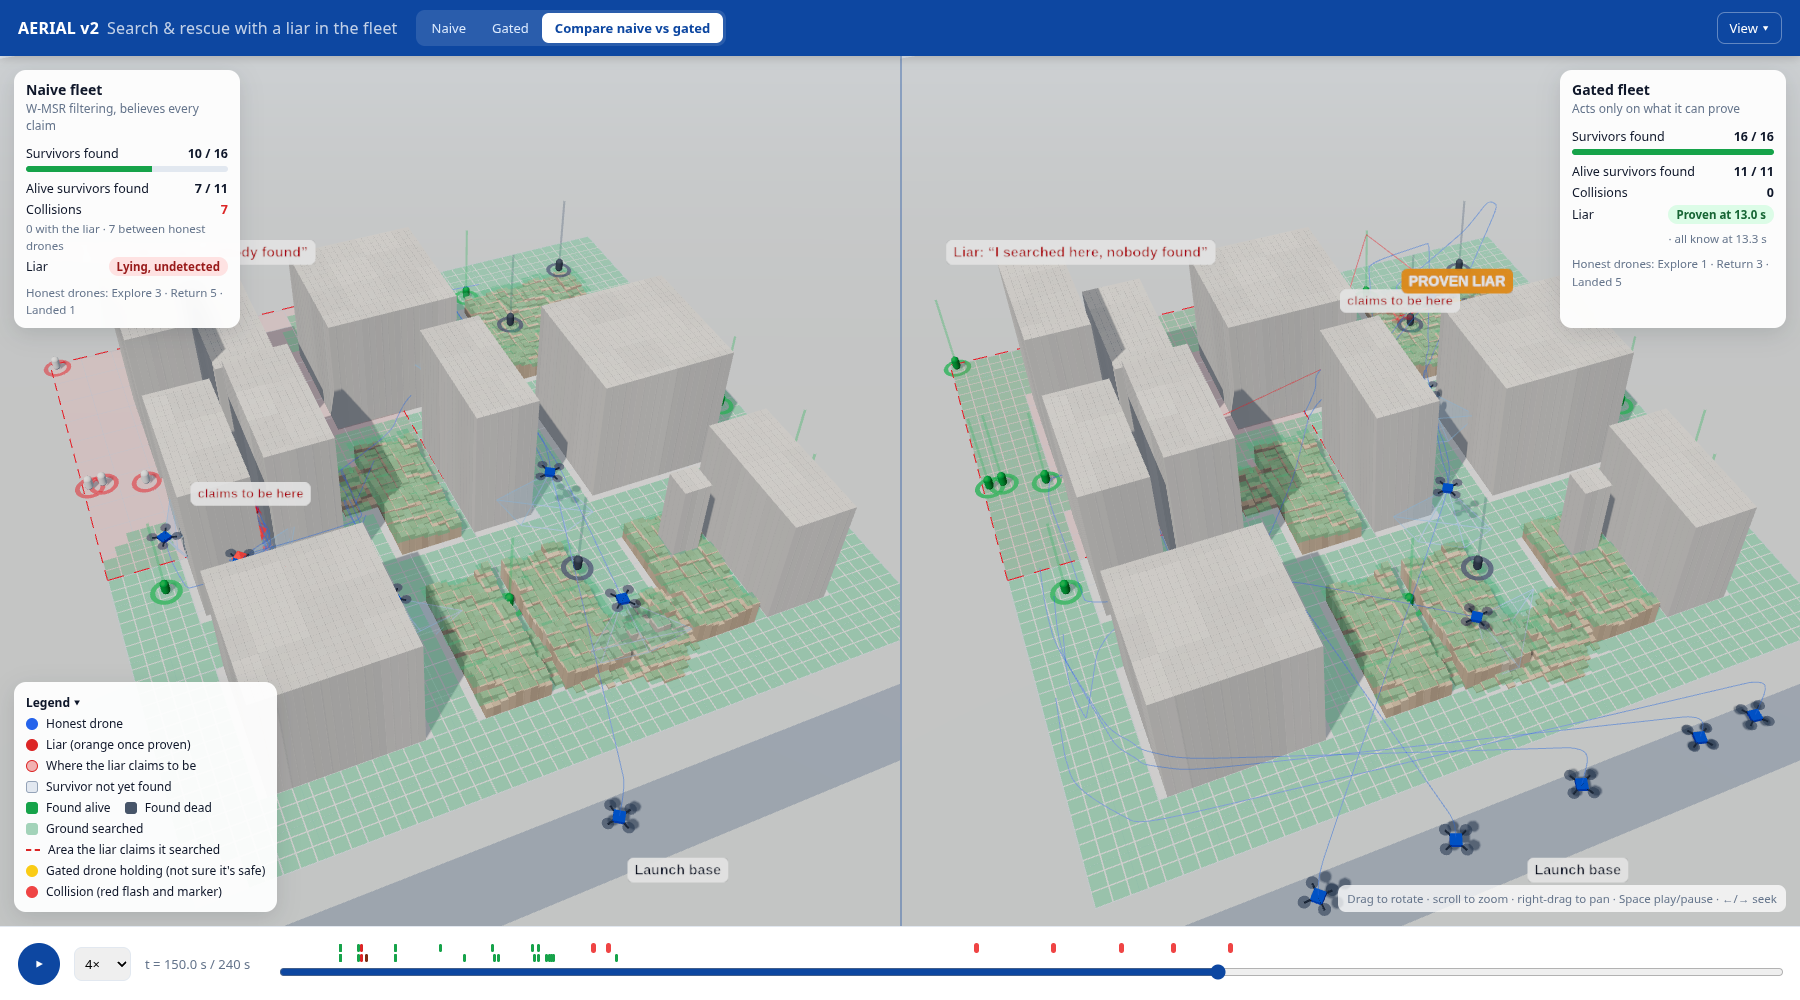
\includegraphics[width=\linewidth]{Figures/results/replay_compare.png}
    \caption[The VeriFly 3D replay: naive vs.\ gated fleet on the same mission]{The VeriFly 3D replay of one
    mission, 150\,s after take-off. Both fleets fly the same district with the same liar (red/orange drone), which
    claims the dashed corner as ``searched, nobody here''. \textbf{Left:} the W-MSR (\emph{naive}) fleet believes the
    claim; the survivors in the corner (red rings) are never found. \textbf{Right:} the \emph{gated} fleet proves
    the liar lied 0.8\,s after it starts lying, reopens the corner and finds all 16 survivors (green: found alive,
    grey: found dead).}
    \label{fig:teaser}
\end{figure}

\section{Goals}
\label{sec:goals}

The project has one scientific goal and several engineering goals that serve it.

\textbf{Scientific goal.} \emph{Quantify the price and the value of acting on knowledge instead of belief} in a
decentralised search-and-rescue fleet with up to $F$ lying members. Measure, under identical conditions, how many
survivors each trust policy finds, how safely it flies, how quickly it identifies the liar, and how long the mission
takes.

\textbf{Objectives.} These were fixed in the proposal and refined during the build:

\begin{table}[h]
\centering
\renewcommand{\arraystretch}{1.25}
\begin{tabularx}{\linewidth}{@{}l X X@{}}
\toprule
\textbf{ID} & \textbf{Objective} & \textbf{How it is met (where in this report)} \\
\midrule
O1 & A faithful, decentralised simulation: unmapped 3D terrain, a limited camera, a lossy multi-hop radio, and no
     agent ever reading the ground truth & Simulator architecture and enforced information boundary
     (\autoref{sec:system-model}, \autoref{sec:architecture}) \\
O2 & A complete mission: transit in formation, exploration with dynamic work division, survivor confirmation, return
     and landing & Mission state machine, geodesic Voronoi partition (\autoref{sec:mission}) \\
O3 & Resilient numeric coordination & W-MSR in formation and survivor localisation
     (\autoref{sec:wmsr}, \autoref{sec:res-localisation}) \\
O4 & Identify liars with \emph{zero} false accusations & S5 possible worlds and sound proof rules R1--R6
     (\autoref{sec:epistemic}, Proposition~\ref{prop:soundness}) \\
O5 & Never act unsafely on unverified claims & Provenance-tagged maps and the knowledge gate
     $\Kn_i\mathit{Safe}$ (\autoref{sec:gate}) \\
O6 & A controlled, statistically sound comparison & Paired randomness, 1,460 server runs, 95\% intervals,
     Wilcoxon tests (\autoref{cp:Results}) \\
O7 & Ground the network assumptions in theory & $\lambda_2$ convergence and $(r,s)$-robustness studies
     (\autoref{sec:res-theory}) \\
\bottomrule
\end{tabularx}
\caption{Project objectives and where each is addressed.}
\label{tab:objectives}
\end{table}

\section{Contributions}
\label{sec:contributions-summary}

\begin{enumerate}
  \item \textbf{A knowledge-gated fleet.} Every drone separates \emph{belief} (someone not yet proven a liar said it),
        which it uses to share out work, from \emph{knowledge} (true in every world consistent with the evidence),
        which it requires before risky actions. Knowledge is computed exactly over all sets of at most $F$ liars.
  \item \textbf{Sound proofs of lying from physics.} Five rules (UWB range, speed, radio horizon, camera, audit) that
        an honest drone provably cannot trigger, plus two weaker kinds of evidence (shared ranges and accusations)
        that only prove ``one of these two lies'', which makes framing impossible by construction.
  \item \textbf{Provenance-tagged maps.} Every coverage, terrain and survivor claim carries a bitmask of the drones
        that vouched for it. When a liar is caught, every claim resting only on its word reverts automatically, and
        the dynamic partition re-sweeps the area with no special re-sweep code.
  \item \textbf{A fair, reproducible experimental framework.} The four fleets share all code and, per seed, all
        random draws. We report 1,460 runs on the departmental GPU server, a 3D web replay, and a set of theory
        studies from a first, 2D build.
\end{enumerate}

\section{Code and Media}
\label{sec:code}

All code, experiment scripts, raw results and figures are in the group repository: \repolink. The
repository README and \tcode{CONTEXT.md} explain how to run every experiment in this report. The interactive 3D replays
(\tcode{docs/media/viewer.html}, \tcode{viewer\_collisions.html}) are single HTML files that open in any browser.

\section{Organisation of the Report}

\autoref{cp:literature} reviews the literature on resilient consensus, epistemic logic, multi-robot coverage and
runtime verification. \autoref{cp:prelim} fixes notation and recalls the theory we build on. \autoref{cp:problem}
formulates the problem, describes the system and the epistemic layer, and proves its key properties.
\autoref{cp:Results} presents the simulation setup, the experiments and their results, and the limitations.
\autoref{cp:Conclusion} concludes. The appendices give the full parameter set and the reproduction recipe, and the
last page lists each member's individual contribution.

\chapter[Literature Review]{Literature Review}
\label{cp:literature}

\parindent0pt

Our system draws on six lines of work: UAVs for disaster response, consensus and its resilient variants, distributed
coverage, information spreading, the logic of knowledge, and secure localisation and safety. This chapter reviews each
briefly and ends by placing our work among them.

\section{UAV Fleets in Disaster Response}

Drones are now a standard tool in disaster management, for damage assessment, mapping, delivery of supplies and
search for victims~\citep{Erdelj2017}. The common architectures are either centralised, where a ground station plans
for all drones, or decentralised, where each drone plans locally from shared information. Centralised planning breaks
down exactly when it is needed most: with ground communication lost, and with drones often out of range of one
another. We therefore follow the decentralised model, in which every drone acts on its own sensors and on information
relayed over a time-varying, multi-hop radio graph.

\section{Consensus and Resilient Consensus}
\label{sec:lit-consensus}

\textbf{Consensus.} \citet{OlfatiSaber2007} survey consensus protocols in which each agent repeatedly moves its state
towards the states of its neighbours. On a connected graph, every agent converges to a common value, and the rate is
governed by the algebraic connectivity $\lambda_2$ of the graph Laplacian~\citep{Fiedler1973, Mesbahi2010}. Formation
control, rendezvous and distributed estimation are all built on this primitive~\citep{Bullo2009}.

\textbf{Byzantine faults.} \citet{Pease1980} and \citet{Lamport1982} showed that agreement in the presence of $F$
arbitrarily misbehaving (Byzantine) agents requires $N > 3F$ agents and enough connectivity, and that signed messages
make the problem much easier. Their model, in which faulty agents can send arbitrary but authenticated messages, is
the one we adopt for the radio layer.

\textbf{W-MSR and network robustness.} \citet{LeBlanc2013} introduced the W-MSR algorithm. Each normal agent discards up
to $F$ neighbour values above its own and up to $F$ below, then averages the rest. They proved that normal agents reach
consensus inside the convex hull of their initial values if and only if the graph is sufficiently \emph{robust}. They
introduced $r$-robustness and $(r,s)$-robustness as the right connectivity notions, replacing the classical vertex
connectivity. \citet{Saldana2017} extended the guarantee to time-varying networks of mobile robots.
\citet{Usevitch2020} gave mixed-integer programs to compute robustness, which is coNP-hard in general.
\citet{Mitra2019} designed Byzantine-resilient distributed observers for estimating a dynamic state. W-MSR is our
\naive{} baseline: it is exactly the resilience a well-designed fleet from this literature would have.

\section{Distributed Coverage and Task Allocation}

\citet{Cortes2004} formulated coverage control as moving agents to the centroids of their Voronoi cells, a rule that
locally optimises a coverage cost and needs only neighbour information. Later work replaced Euclidean distance with
geodesic distance in non-convex environments, so that a cell behind a wall belongs to the agent that can actually
reach it. Our fleet uses a \emph{geodesic Voronoi partition} computed by multi-source Dijkstra~\citep{Dijkstra1959}
over the drone's own map. Each drone computes it locally, and work-stealing balances the load when a region empties.

\section{Information Spreading}

Gossip, or epidemic, protocols spread information through a network by having each node forward new items to its
neighbours~\citep{Demers1987}. Their simple-contagion dynamics follow the SI model taught in the course. We use gossip for
all fleet-wide news (cleared cells, survivors, terrain, accusations). We show that accusations of lying cannot spread
as a simple contagion. Because a single accuser could itself be the liar, belief in an accusation must follow a
\emph{threshold} rule (\autoref{sec:accusations}).

\section{Knowledge and Possible Worlds}
\label{sec:lit-epistemic}

Epistemic logic formalises what an agent \emph{knows}. In Kripke semantics~\citep{Kripke1963}, an agent knows $\varphi$
in a world $w$ if $\varphi$ is true in every world the agent cannot distinguish from $w$. When indistinguishability is an
equivalence relation, this is the logic S5. \citet{Fagin1995} developed this theory for distributed systems.
\citet{Halpern1990} used it to prove that common knowledge cannot be attained over unreliable channels.
\citet{vanDitmarsch2007} treat how knowledge changes as evidence arrives, which is our setting: every proof of lying is
a public or private announcement that removes worlds. Knowledge-based programs, which condition actions on knowledge
tests such as ``if $\Kn_i\varphi$ then act'', are a central idea in that literature. Our motion gate is a direct
instance of one.

\section{Secure Localisation, Spoofing and Safety}

\textbf{Verifying positions.} A drone that lies about its position can be caught only with a measurement it cannot
forge. \citet{Capkun2005} showed that time-of-flight ranging (as in ultra-wideband radios) gives \emph{verifiable}
distance bounds, because a node can make itself appear farther away by delaying its reply, but never closer. With
three or more verifiers around it, a position claim can be checked by multilateration. \citet{Gil2017} used physical
properties of wireless signals to detect spoofed robot identities in multi-robot networks. Our proof rules R1 (range)
and R6 (shared range) follow the same principle: a claim is checked against a physical measurement taken by the
listener.

\textbf{Collision avoidance.} Velocity obstacles~\citep{Fiorini1998} and control barrier functions~\citep{Ames2019}
are standard tools for keeping robots apart. Both assume that the robot knows where its neighbours are. When a
neighbour may be lying, its reported position cannot be trusted. Our knowledge gate therefore checks a manoeuvre
against \emph{every} position a neighbour could occupy in \emph{every} world the drone cannot rule out.

\section{Runtime Verification and Sequential Testing}

Signal Temporal Logic (STL)~\citep{Maler2004} expresses requirements over continuous signals, such as ``always keep
1\,m separation'' or ``eventually find survivor 7''. Its \emph{robustness} semantics~\citep{Donze2010} returns a real
number whose sign says whether the requirement held and whose size says by how much. We use STL robustness to grade
every run offline. For deciding whether a found survivor is alive, we use Wald's Sequential Probability Ratio
Test~\citep{Wald1945}. It needs the fewest observations on average for given error rates, so a drone hovers only as
long as needed.

\section{Positioning of this Work}

\begin{table}[h]
\centering
\renewcommand{\arraystretch}{1.25}
\begin{tabularx}{\linewidth}{@{}X c c c c@{}}
\toprule
\textbf{Approach} & \textbf{Numeric} & \textbf{Claims} & \textbf{Identifies} & \textbf{Safe w.r.t.} \\
                  & \textbf{resilience} & \textbf{verified} & \textbf{liars} & \textbf{lying peers} \\
\midrule
Plain consensus~\citep{OlfatiSaber2007}           & \xmark & \xmark & \xmark & \xmark \\
W-MSR / robust networks~\citep{LeBlanc2013}       & \cmark & \xmark & \xmark & \xmark \\
Spoof detection~\citep{Gil2017}                    & \xmark & partly & \cmark & \xmark \\
Collision avoidance~\citep{Fiorini1998,Ames2019}   & \xmark & \xmark & \xmark & \xmark \\
\textbf{VeriFly gated fleet (ours)}                & \cmark & \cmark & \cmark & \cmark \\
\bottomrule
\end{tabularx}
\caption{What each line of work provides for a search fleet with lying members.}
\label{tab:positioning}
\end{table}

To our knowledge, no prior system combines resilient numeric consensus with exact possible-worlds knowledge of
\emph{who} is lying, provenance-tagged shared maps, and a knowledge-based motion gate, all evaluated in a decentralised
3D search mission with a controlled, paired comparison. The contribution is not a new consensus algorithm. It is a
demonstration, with numbers, that the decision layer above consensus is where a search fleet's resilience is decided.

\chapter[Preliminaries]{Notations \& Preliminaries}
\label{cp:prelim}

\parindent0pt

\section{Notations}
\label{sec:notation}

\subsection{Agents, Space and Time}

\begin{table}[h]
\centering
\renewcommand{\arraystretch}{1.2}
\begin{tabularx}{\linewidth}{@{}l X@{}}
\toprule
\textbf{Symbol} & \textbf{Meaning} \\
\midrule
$\mathcal{V}=\{0,\dots,N-1\}$ & the drones; $N=10$ by default \\
$F$ & the assumed maximum number of liars ($F\le 2$) \\
$\mathcal{S}^\star\subseteq\mathcal{V}$ & the true set of liars, $|\mathcal{S}^\star|\le F$, unknown to the honest drones \\
$\mathcal{N}=\mathcal{V}\setminus\mathcal{S}^\star$ & the honest (normal) drones \\
$t,\ \Delta t$ & time and the simulation tick, $\Delta t = 0.1$\,s \\
$p_i,\ v_i\in\mathbb{R}^3$, $\psi_i$ & true position, velocity and heading of drone $i$ \\
$u_i\in\mathbb{R}^3$ & commanded acceleration, $\|u_i\|\le a_{\max}$ \\
$\hat p_j,\ \hat v_j$ & position and velocity \emph{claimed} by drone $j$ in its beacon \\
$r_{ij}$ & UWB range from $i$ to $j$ measured with $j$'s packet, $|r_{ij}-\|p_i-p_j\||\le\varepsilon'$ \\
$H(x,y)$ & ground-truth terrain height (2.5D height map, 1\,m raster) \\
$[\ell_c,\,h_c]$ & a drone's interval belief on the ground height of terrain cell $c$ \\
$\mathcal{C}$ & the coverage grid over the search zone: $50\times50 = 2{,}500$ cells of $2\times2$\,m \\
\bottomrule
\end{tabularx}
\caption{Notation for agents, space and time.}
\label{tab:notation-agents}
\end{table}

\subsection{Communication and Knowledge}

\begin{table}[h]
\centering
\renewcommand{\arraystretch}{1.2}
\begin{tabularx}{\linewidth}{@{}l X@{}}
\toprule
\textbf{Symbol} & \textbf{Meaning} \\
\midrule
$\mathcal{G}(t)=(\mathcal{V},\mathcal{E}(t))$ & directed communication graph at tick $t$; $(j,i)\in\mathcal{E}(t)$ iff $i$
received $j$'s packet \\
$R,\ p_{\mathrm{drop}}$ & radio range (35\,m) and independent packet-loss probability (0.1) \\
$\mathcal{N}_i(t)$ & in-neighbours of $i$ at tick $t$ \\
$L$ & silence threshold: ticks without a packet after which $j$ is assumed out of range \\
$\rho_c\in\{0,1\}^N$ & provenance bitmask of a claim about cell $c$: bit $j$ set iff drone $j$ vouched for it \\
$\Hyp_i\subseteq 2^{\mathcal{V}}$ & drone $i$'s surviving \emph{worlds}: candidate liar sets $S$ with $|S|\le F$, $i\notin S$ \\
$\Kn_i\varphi$ & ``$i$ knows $\varphi$'': $\varphi$ holds in every world of $\Hyp_i$ \\
$\Bl_i\varphi$ & ``$i$ believes $\varphi$'': some drone not proven a liar reported $\varphi$ \\
$q$ & audit fraction: share of each teammate's cleared claims re-checked (0.1) \\
$\tau,\ d_{\mathrm{safe}}$ & gate look-ahead after one tick (0.3\,s) and the separation that counts as a collision (1\,m) \\
\bottomrule
\end{tabularx}
\caption{Notation for communication, provenance and knowledge.}
\label{tab:notation-knowledge}
\end{table}

\section{Background on Preliminaries}
\label{sec:background}

\subsection{Graphs, Consensus and Algebraic Connectivity}

Let $A(t)$ be the adjacency matrix of $\mathcal{G}(t)$ and $L(t)=D(t)-A(t)$ its Laplacian, where $D$ is the diagonal
in-degree matrix. In the linear consensus protocol
\begin{equation}
    \dot x_i = \sum_{j\in\mathcal{N}_i} a_{ij}\,(x_j - x_i), \qquad \text{i.e.}\quad \dot x = -L x ,
    \label{eq:consensus}
\end{equation}
all states converge to a common value on a connected undirected graph. The slowest mode decays as
$e^{-\lambda_2 t}$, where $\lambda_2$ is the second-smallest Laplacian eigenvalue, the \emph{algebraic
connectivity}~\citep{Fiedler1973}. For the second-order (double-integrator) agents used in formation flight, the rate
also depends on the position and velocity gains $k_p$ and $k_v$. It grows with $\lambda_2$ until it saturates at a
limit set by the gains. We verify this behaviour in \autoref{sec:res-theory}.

\subsection{Resilient Consensus: W-MSR and Network Robustness}
\label{sec:wmsr}

\begin{definition}[W-MSR~\citep{LeBlanc2013}]
At each step, a normal agent $i$ with value $x_i$ sorts the values received from its neighbours. If at least $F$
values are larger than $x_i$, it removes the $F$ largest; otherwise it removes all values larger than $x_i$. It
does the same for values smaller than $x_i$. It then updates to a weighted average of its own value and the
remaining values. In our implementation all weights are equal:
\begin{equation}
    x_i \leftarrow \frac{1}{1+|\mathcal{R}_i|}\Big(x_i + \sum_{j\in\mathcal{R}_i} x_j\Big),
    \label{eq:wmsr}
\end{equation}
where $\mathcal{R}_i$ is the set of neighbours not removed.
\end{definition}

The guarantee depends on how well connected the graph is, measured by \emph{robustness}.

\begin{definition}[$r$-reachable, $r$-robust, $(r,s)$-robust~\citep{LeBlanc2013}]
A nonempty set $S\subset\mathcal{V}$ is \emph{$r$-reachable} if some $i\in S$ has at least $r$ neighbours outside $S$.
A graph is \emph{$r$-robust} if, for every pair of nonempty disjoint subsets $S_1,S_2\subset\mathcal{V}$, at least
one of them is $r$-reachable. It is \emph{$(r,s)$-robust} if, for every such pair, with
$\mathcal{X}^r_{S}=\{i\in S : |\mathcal{N}_i\setminus S|\ge r\}$, at least one of the following holds:
$|\mathcal{X}^r_{S_1}|=|S_1|$, $|\mathcal{X}^r_{S_2}|=|S_2|$, or $|\mathcal{X}^r_{S_1}|+|\mathcal{X}^r_{S_2}|\ge s$.
\end{definition}

\begin{lemma}[\citet{LeBlanc2013}]
\label{lem:wmsr}
Under the $F$-total malicious model, W-MSR guarantees that the normal agents reach consensus within the convex hull of
their initial values if and only if the network is $(F+1,F+1)$-robust. Under the $F$-local model, $(2F+1)$-robustness
is sufficient. In both cases, every value a normal agent adopts lies within the range of normal values: a value that
survives trimming is bracketed by trimmed values, and at least one of those came from a normal agent.
\end{lemma}

Lemma~\ref{lem:wmsr} is precisely what W-MSR \emph{does} guarantee, and it shows what it does not. A liar that reports a
value inside the normal range survives the trimming forever, and a non-numeric claim cannot be trimmed at all.

\subsection{Epistemic Logic and Possible Worlds}
\label{sec:prelim-epistemic}

A Kripke structure $M=(W,\{\sim_i\},V)$ consists of a set of worlds $W$, an indistinguishability relation $\sim_i$ for
each agent, and a valuation $V$ that says which atomic facts hold in which world. Agent $i$ \emph{knows} $\varphi$ at
world $w$, written $M,w\models\Kn_i\varphi$, if $M,w'\models\varphi$ for every $w'$ with $w\sim_i w'$. When each
$\sim_i$ is an equivalence relation, $\Kn_i$ satisfies the S5 axioms~\citep{Fagin1995}:
\begin{align}
    \textbf{K:}&\ \ \Kn_i(\varphi\rightarrow\psi)\rightarrow(\Kn_i\varphi\rightarrow\Kn_i\psi) &
    \textbf{T:}&\ \ \Kn_i\varphi\rightarrow\varphi \\
    \textbf{4:}&\ \ \Kn_i\varphi\rightarrow\Kn_i\Kn_i\varphi &
    \textbf{5:}&\ \ \neg\Kn_i\varphi\rightarrow\Kn_i\neg\Kn_i\varphi
\end{align}
Axiom \textbf{T} (truth) matters most here: what is known is true. We need it to hold for statements such as ``drone
$j$ is a liar'', because an honest drone acting on a false accusation would be worse than acting on nothing.

\textbf{Worlds in VeriFly.} The only thing a drone does not know about the \emph{structure} of the fleet is who the liars are.
So a world is a candidate liar set $S\subseteq\mathcal{V}$ with $|S|\le F$ and $i\notin S$. Drone $i$ starts with all
\begin{equation}
    |\Hyp_i(0)| \;=\; \sum_{k=0}^{F}\binom{N-1}{k}
    \label{eq:nworlds}
\end{equation}
of them: 10 worlds for $N=10$, $F=1$, and 191 for $N=20$, $F=2$. Evidence is an \emph{announcement} that removes worlds
inconsistent with it~\citep{vanDitmarsch2007}. Then
$\Kn_i(j\in\mathcal{S}^\star)\iff j\in S\ \forall S\in\Hyp_i$ and
$\Kn_i(j\notin\mathcal{S}^\star)\iff j\notin S\ \forall S\in\Hyp_i$.

\subsection{Sequential Probability Ratio Test}

To decide between hypotheses $\mathsf{H}_1$ (alive) and $\mathsf{H}_0$ (dead) from a stream of independent observations
$z_1,z_2,\dots$, Wald's SPRT~\citep{Wald1945} accumulates the log-likelihood ratio
\begin{equation}
    \Lambda_n = \log\frac{P(\mathsf{H}_1)}{P(\mathsf{H}_0)} + \sum_{k=1}^{n}\log\frac{p(z_k\mid\mathsf{H}_1)}{p(z_k\mid\mathsf{H}_0)}
\end{equation}
and stops as soon as $\Lambda_n$ leaves an interval $(a,b)$. We stop when the posterior $P(\text{alive})$ exceeds 0.95
or falls below 0.05. Among all tests with the same error probabilities, the SPRT minimises the expected number of
observations.

\subsection{Signal Temporal Logic}

STL formulas over a real-valued signal $s(t)$ are built from predicates $\mu \equiv f(s(t))\ge 0$ with Boolean
connectives and the timed operators \emph{always} $\mathbf{G}_{[a,b]}$ and \emph{eventually} $\mathbf{F}_{[a,b]}$. The
quantitative robustness $\rho$~\citep{Donze2010} is defined recursively:
\begin{equation}
    \rho(\mu,t)=f(s(t)),\quad \rho(\mathbf{G}_{[a,b]}\varphi,t)=\min_{t'\in[t+a,t+b]}\rho(\varphi,t'),\quad
    \rho(\mathbf{F}_{[a,b]}\varphi,t)=\max_{t'\in[t+a,t+b]}\rho(\varphi,t').
\end{equation}
$\rho>0$ means the requirement is satisfied with margin $\rho$, and $\rho<0$ means it is violated.

\chapter[Problem Formulation]{Problem Formulation}
\label{cp:problem}

\parindent0pt

\section{Problem Statement}
\label{sec:problem}

A fleet of $N$ drones takes off from a launch strip next to a square search zone in which an earthquake has collapsed
part of the buildings at random. Somewhere in the zone are $n_s=16$ survivors. The drones have \emph{no map}. They must
find as many survivors as possible, decide whether each one is alive, avoid collisions with the terrain and with each
other, and land again. Up to $F$ drones are \emph{liars} whose identity the others do not know. This section fixes the
world, drone, radio and adversary models, states the assumptions, and splits the mission into execution phases.

\subsection{System Model}
\label{sec:system-model}

\textbf{World.} The arena is a $120\times120$\,m square, represented as a 2.5D height map $H(x,y)$ on a 1\,m raster.
City blocks about 20\,m wide are separated by streets 8--12\,m wide. Each block holds one or two buildings 12--35\,m
tall, so many of them are taller than the drones' 15\,m ceiling and must be flown \emph{around}. Each building collapses
independently with probability $0.4$. It then becomes a rubble mound 1--5\,m high, with debris spilling into a
neighbouring street, and about a third of collapses leave a tall pile of 13--18\,m. The search zone is the central
$100\times100$\,m square, divided into the coverage grid $\mathcal{C}$ of $2{,}500$ cells. Survivors sit at cell centres
and are placed only in cells that some legal camera pose can see, so no fleet is penalised for missing a person under a
roof. Each survivor is alive with probability $0.7$. In the scenario used for demonstrations, a $50\times50$\,m corner
of the zone is the area the liar will claim, and at least three survivors are placed deep inside it.

\textbf{Drones.} Each drone is a 3D double integrator with heading:
\begin{equation}
    \dot p_i = v_i,\qquad \dot v_i = u_i,\qquad \|u_i\|\le 4\,\mathrm{m/s^2},\quad \|v_i^{xy}\|\le 5\,\mathrm{m/s},
    \quad |v_i^{z}|\le 2\,\mathrm{m/s},\quad |\dot\psi_i|\le 90^\circ\!/\mathrm{s}.
    \label{eq:dynamics}
\end{equation}
Drones fly between 4 and 15\,m. For vertical separation, drone $i$ cruises on layer $z_i\in\{6,9,12\}$\,m, chosen as
$i \bmod 3$. Each drone carries one forward-facing camera, tilted $30^\circ$ down, with a $90^\circ\times60^\circ$ field
of view, a 25\,m depth range and a 5\,Hz frame rate. It is simulated by marching $32\times12=384$ rays over the height
map. From each frame a drone obtains (i) terrain facts (``the ground here is below this ray'', ``the ground here is at
least this high''), (ii) the coverage cells it has \emph{viewed}, (iii) a noisy look at each survivor in a viewed cell,
and (iv) sightings of other drones inside its view volume.

\textbf{Radio.} Every tick, drone $i$ receives drone $j$'s packet if $\|p_i-p_j\|\le R=35$\,m and an independent
Bernoulli($1-p_{\mathrm{drop}}$) draw succeeds, with $p_{\mathrm{drop}}=0.1$. Losses are independent per direction, so
$\mathcal{G}(t)$ is a time-varying \emph{directed} graph. Every received packet also yields a UWB time-of-flight range
$r_{ij}$, equal to the true distance plus noise $\mathcal{N}(0,0.05^2)$ clipped at $\pm4\sigma=\pm0.2$\,m. There are
two kinds of traffic:
\begin{itemize}
    \item \textbf{beacons}: ``I am at $\hat p_j$, moving at $\hat v_j$'', sent every tick and heard by direct
          neighbours only;
    \item \textbf{events}: news for the whole fleet (cells cleared, survivor found, terrain seen, ``I have proof that
          $j$ lied''). Events spread by gossip: each drone forwards each new event once, one hop per tick, at most 64
          per tick, in priority order: accusations, then survivors, then coverage, then terrain.
\end{itemize}

\textbf{Adversary.} At most $F$ drones are liars. A liar runs the same code with the same sensors and has \emph{no access
to the ground truth}. It flies honestly during transit and starts lying at $t=12$\,s. It may: lie about its own
position and velocity in its beacons; claim cells ``cleared, nobody here'' that it never viewed; hide every survivor it
sees; and refuse to relay others' events. It may not forge the origin of another drone's message, alter a UWB range,
or send different content to different listeners.

\subsection{Assumptions}
\label{sec:assumptions}

\begin{assumption}[Bounded faults] At most $F$ drones lie, and $F$ is known to every drone. \end{assumption}
\begin{assumption}[Authenticated broadcast] Every message carries its true sender (signatures are modelled abstractly)
and is broadcast, so a liar cannot impersonate others or equivocate. \end{assumption}
\begin{assumption}[Physical ranging] $|r_{ij}-\|p_i-p_j\||\le\varepsilon' = 0.2$\,m for every received packet. \end{assumption}
\begin{assumption}[Deterministic detection] A survivor is detected if and only if its cell is viewed, and survivors do
not move. Only the alive/dead judgement is noisy. \end{assumption}
\begin{assumption}[Drone visibility] A drone inside another drone's view volume (within 20\,m, in line of sight) is
always sighted. \end{assumption}
\begin{assumption}[Static world] The terrain does not change during a mission. There is no wind, and drones are points. \end{assumption}
\begin{assumption}[Silence] A drone not heard for $L=\lceil \ln 10^{-9}/\ln p_{\mathrm{drop}}\rceil=9$ consecutive
ticks was out of radio range during that window. This is the \emph{only} probabilistic assumption in the safety
argument; it fails with probability below $10^{-9}$. \end{assumption}
\begin{assumption}[No ramming] Liars are not suicidal: a liar does not deliberately accelerate into another drone. A
gate can only control the drone's own motion. \end{assumption}

\begin{keybox}[The single most important design choice]
One function, $\mathrm{viewed}(c,\text{pose})$, decides ``seen'' for \emph{both} coverage and survivor detection. A cell
is viewed if its centre point lies inside the camera frustum, within 15\,m, in line of sight, and at least $20^\circ$
below the horizon. Because detection is exact for viewed cells, ``I looked at this cell and nobody was there'' becomes a
\emph{hard fact}. This is what later lets an audit \emph{prove} that a teammate lied.
\end{keybox}

\subsection{Execution Phase \#1: Transit and Formation}

All drones take off from the launch strip and fly to individual \emph{entry slots} spread evenly along the southern edge
of the zone, each at its own layer. To keep the line together, each drone combines the forward progress of the
neighbours it hears using W-MSR (\autoref{eq:wmsr}). It stays at most 4\,m ahead of the filtered value and is pulled
towards it by half the gap. The unfiltered reference fleet uses the plain mean instead. Transit ends at the entry slot
or after 30\,s at the latest. The liar behaves honestly in this phase.

\subsection{Execution Phase \#2: Exploration, Confirmation and Verification}

Each drone repeatedly chooses an unsearched cell in its own region, plans a route through space it knows to be free,
flies there, and looks. When it spots a survivor, it hovers until it can decide alive or dead (at most 8\,s). When nothing
is left to search, a gated drone \emph{audits} a random sample of its teammates' claims. Then it returns to its landing
slot. Whenever new work appears, for example because a liar has just been exposed and its claimed area has reopened,
the drone drops back into exploration. The mission ends when every honest drone has landed or the time limit is reached.

\subsection{Formal Objectives}

Let $\mathcal{F}(T)$ be the set of survivors detected by an honest drone's own camera by time $T$. For every fleet we
measure, per mission:
\begin{itemize}
    \item \textbf{effectiveness}: $|\mathcal{F}(T)|/n_s$ (survivors found), and the number missed inside the liar's
          claimed area;
    \item \textbf{safety}: collisions, i.e.\ pairs of drones closer than $d_{\mathrm{safe}}=1$\,m, together with the
          STL robustness of $\varphi_{\mathrm{safe}}$ (\autoref{sec:stl});
    \item \textbf{knowledge}: the time at which the first and the last honest drone \emph{knows} each liar, and the
          number of \emph{false accusations}, which must be zero;
    \item \textbf{cost}: completion time (all honest drones landed).
\end{itemize}
The design problem is to choose each drone's local decision rule so that the fleet finds every survivor and never
accuses an honest drone, whatever the (bounded) liars do, at the smallest possible cost in time.

\section{Solution Approach}
\label{sec:solution}

\subsection{Architecture: Simulator as Reality, Agents as Onboard Computers}
\label{sec:architecture}

The code is split into two roles with an enforced boundary (\autoref{fig:architecture}). The \textbf{simulator}
plays reality: it alone knows the terrain, the survivors and every drone's true pose. Each \textbf{agent} is a drone's
onboard computer: it receives only its own observation (its camera frame, its inbox, its UWB ranges) and returns a
command. A unit test fails if any agent module imports the ground-truth world package, so no agent can secretly peek
at the truth. All four fleets share the same agent class.

\begin{figure}[t]
\centering
\begin{tikzpicture}[
    font=\small,
    stage/.style={draw=boxblue, fill=boxbg, rounded corners=3pt, thick, align=center, minimum width=2.45cm,
                  minimum height=1.05cm, text width=2.35cm},
    hot/.style={stage, draw=orange!80!black, fill=orange!12},
    flow/.style={-{Stealth[length=2.4mm]}, thick, boxblue},
    ]
  \node[stage] (b) at (0,0)      {\textbf{1. Beacons}\\ every drone states $\hat p_j,\hat v_j$};
  \node[stage] (s) at (3.2,0)    {\textbf{2. Sensing}\\ camera (5\,Hz), UWB ranges};
  \node[stage] (c) at (6.4,0)    {\textbf{3. Radio}\\ disk graph, drops, gossip};
  \node[hot]   (d) at (9.6,0)    {\textbf{4. Decide}\\ each drone, own inbox only};
  \node[stage] (p) at (6.4,-2.1) {\textbf{5. Physics}\\ double integrator};
  \node[stage] (r) at (3.2,-2.1) {\textbf{6. Record}\\ metrics, replay};
  \draw[flow] (b) -- (s);
  \draw[flow] (s) -- (c);
  \draw[flow] (c) -- (d);
  \draw[flow] (d.south) |- (p.east);
  \draw[flow] (p) -- (r);
  \draw[flow] (r.west) -| (b.south);
  \node[font=\footnotesize\itshape, text=gray] at (4.8,-1.05) {one tick $=0.1$\,s};
  \begin{scope}[on background layer]
    \node[draw=gray!60, dashed, rounded corners=4pt, fit=(b)(s)(c)(p)(r), inner sep=7pt,
          label={[font=\footnotesize, text=gray]above left:simulator (ground truth)}] {};
    \node[draw=orange!70!black, dashed, rounded corners=4pt, fit=(d), inner sep=7pt,
          label={[font=\footnotesize, text=orange!60!black]above:agents}] {};
  \end{scope}
\end{tikzpicture}
\caption[One simulation tick and the information boundary]{One simulation tick. Steps 1--3 and 5--6 belong to the
simulator, which holds the ground truth. In step 4 each agent sees only its own observation. Beacons, camera frames and
UWB ranges are produced at the \emph{same} tick, so an honest drone that is simply moving can never appear to lie.}
\label{fig:architecture}
\end{figure}

\textbf{Paired randomness.} All randomness (packet drops, range noise, sensor noise, liar choices) comes from named
random streams derived from one seed, and every stream draws a full block every tick, whatever the drones do. When the
\naive{} and \gated{} fleets fly the same seed, they therefore see exactly the same lost packets and the same noise. The
experiment runner checks this and refuses to report a comparison if the two runs drew different random numbers. A
difference between fleets is caused by trust, not by luck.

\subsection{Mapping Unknown Terrain: Intervals, not Guesses}

Each drone keeps, for every 1\,m terrain cell $c$, an interval $[\ell_c,h_c]$ that must contain the true height. It
starts at $[0,\infty)$:
\begin{itemize}
    \item a camera ray that passes \emph{over} the cell at height $z$ proves $H<z$, so $h_c\leftarrow\min(h_c,z)$;
    \item a ray that \emph{hits} the cell at height $z$ proves only $H\ge z$, so $\ell_c\leftarrow\max(\ell_c,z)$.
\end{itemize}
A cell is free on layer $z_i$ only if $h_c+1.5\,\mathrm{m}\le z_i$. Unknown space is therefore \emph{never} treated as
free. Recording a wall hit as ``the height'' would be a serious error, since the air above a 35\,m tower would then
look free. Every second, each drone relays the cells it newly knows to be free and the walls it has seen. Receivers
store each report under its reporter's bit. Terrain claims thus pass through exactly the same trust machinery as
coverage claims, and a liar cannot lure drones into a building by calling it open air.

\subsection{Mission Logic and Dynamic Work Division}
\label{sec:mission}

\begin{figure}[t]
\centering
\begin{tikzpicture}[
    font=\small,
    mode/.style={draw=boxblue, fill=boxbg, rounded corners=3pt, thick, minimum width=1.9cm, minimum height=0.9cm,
                 font=\small\bfseries},
    hmode/.style={mode, draw=orange!80!black, fill=orange!12},
    desc/.style={font=\scriptsize, text width=2.0cm, align=center, text=black!75},
    flow/.style={-{Stealth[length=2.2mm]}, thick, boxblue},
    ]
  \node[mode]  (t) at (0,0)    {Transit};
  \node[mode]  (e) at (2.75,0) {Explore};
  \node[mode]  (c) at (5.5,0)  {Confirm};
  \node[hmode] (a) at (8.25,0) {Audit};
  \node[mode]  (r) at (11,0)   {Return};
  \node[desc, below=0.25cm of t] {W-MSR formation to entry slot};
  \node[desc, below=0.25cm of e] {pick, plan, fly, look; steal work};
  \node[desc, below=0.25cm of c] {hover, SPRT alive/dead ($\le 8$\,s)};
  \node[desc, below=0.25cm of a] {\textbf{gated only}: re-check $q$ of claims};
  \node[desc, below=0.25cm of r] {fly to slot, land};
  \draw[flow] (t) -- (e);
  \draw[flow] ([yshift=3pt]e.east) -- ([yshift=3pt]c.west);
  \draw[flow] ([yshift=-3pt]c.west) -- ([yshift=-3pt]e.east);
  \draw[flow] (c) -- node[above, font=\scriptsize] {done} (a);
  \draw[flow] (a) -- (r);
  \draw[flow, orange!80!black, very thick] (r.north) to[bend right=32]
       node[above, font=\scriptsize, text=orange!60!black] {cells reopen (liar caught)} (e.north);
\end{tikzpicture}
\caption[The per-drone mission state machine]{The per-drone mission state machine. Back-edges into \emph{Explore}
fire whenever undone cells reappear, for example when a liar's claims are discarded. This is how the re-sweep happens
without any special-case code.}
\label{fig:modes}
\end{figure}

\textbf{Who goes where: a geodesic Voronoi partition.} Once a second, every drone computes a partition of the coverage
grid \emph{locally}. It takes its own position and the last known positions of its teammates (from beacons, and from
POSE events relayed at 1\,Hz, at most 15\,s old), runs one multi-source Dijkstra search over its 2\,m navigation grid,
and labels every cell with the drone that can reach it soonest \emph{by flight path}. Walls block the search, while
unknown cells count as passable, so distances to unexplored space remain meaningful. The gated fleet leaves out any drone
it has proven to be a liar. No negotiation is needed: drones holding the same information compute the same partition,
and small disagreements cost only a little duplicate work.

\textbf{Choosing the next target.} Candidates are the cells of the drone's own region that are not yet \emph{done}, where
done means swept, holding a reported survivor, under a roof, or given up after three failed viewing attempts. If the
region is finished, the drone steals unfinished cells from anywhere. It scores candidates by Dijkstra path length over
cells free on its layer, keeps its current target unless another is at least 6\,m better (hysteresis), flies to the
frontier when the target lies in unknown space, and turns on the spot before any turn larger than $45^\circ$, so that the
camera has looked where the drone is about to go.

\textbf{Safety reflexes} are never gated: every drone is pushed away from neighbours closer than 3\,m, from known walls
within 3\,m, and from the arena boundary. ``Closing in'' is computed from the drone's \emph{own} velocity, so a liar
cannot fake an approach.

\subsection{Four Fleets, One Program}
\label{sec:fleets}

The fleets differ only in trust (\autoref{tab:fleets}). In the main sweep, the \naive{} fleet also runs the predictive
motion gate, but it believes every report (\tcode{mission.trust\_gate}), so that \emph{only} trust differs between
\naive{} and \gated{}.

\begin{table}[h]
\centering
\renewcommand{\arraystretch}{1.25}
\begin{tabularx}{\linewidth}{@{}l X c c c c@{}}
\toprule
\textbf{Fleet} & \textbf{Whose claims it acts on} & \textbf{Numbers} & \textbf{Lie checks} & \textbf{Audits} &
\textbf{Gate} \\
\midrule
unfiltered & everyone, even proven liars & mean & \xmark & \xmark & \xmark \\
\naive{}   & anyone not proven a liar (it never checks, so: everyone) & W-MSR & \xmark & \xmark & believes all$^\dagger$ \\
\gated{}   & belief to share out work; \textbf{knowledge} to act and judge ``done'' & W-MSR & \cmark & \cmark & $\Kn_i\mathit{Safe}$ \\
oracle     & told the true liars at $t=0$ & W-MSR & not needed & \xmark & $\Kn_i\mathit{Safe}$ \\
\bottomrule
\end{tabularx}
\caption[The four fleets]{The four fleets. $^\dagger$\,In the sweep, E1 and E2 the naive fleet runs the motion
gate with every report believed. In the first E1 round (\autoref{app:verification}) it had no gate.}
\label{tab:fleets}
\end{table}

\subsection{The Epistemic Layer: Knowing who Lies}
\label{sec:epistemic}

Each gated drone $i$ maintains the world set $\Hyp_i$ of \autoref{sec:prelim-epistemic}, stored as an array of
64-bit masks, together with a flag per world saying whether it is still alive. Evidence comes in two forms:
\begin{itemize}
    \item a \textbf{unit} $\mathsf{Unit}(j)$, a \emph{proof} that $j$ lied, which removes every world in which $j$ is honest;
    \item a \textbf{clause} $\mathsf{Clause}(\{j,k\})$, proof that $j$ \emph{or} $k$ lied, which removes every world
          in which both are honest.
\end{itemize}

\begin{table}[h]
\centering
\renewcommand{\arraystretch}{1.3}
\begin{tabularx}{\linewidth}{@{}c l X l@{}}
\toprule
\textbf{Rule} & \textbf{Check} & \textbf{Condition (from $j$'s packet received by $i$)} & \textbf{Evidence} \\
\midrule
R1 & range   & $\big|\,\|\hat p_j-p_i\| - r_{ij}\big| > \varepsilon'$ for a beacon of the current tick & $\mathsf{Unit}(j)$ \\
R2 & speed   & $\|\hat v_j^{xy}\|>v_h$ or $|\hat v_j^z|>v_z$, or two of $j$'s own claims further apart than the limits allow & $\mathsf{Unit}(j)$ \\
R3 & horizon & $\|\hat p_j-p_i\|>R+\varepsilon'$, yet the packet was received & $\mathsf{Unit}(j)$ \\
R4 & camera  & $\hat p_j$ lies in the volume $i$'s camera sees empty (with margin), and no drone is sighted near it & $\mathsf{Unit}(j)$ \\
R5 & audit   & $i$'s own camera detects a survivor in a cell $j$ claimed ``cleared, nobody here'' & $\mathsf{Unit}(j)$ \\
R6 & shared range & drone $k$'s reported range to $j$ for beacon $s$ contradicts $j$'s claim $s$ by more than $2\varepsilon'$ & $\mathsf{Clause}(\{j,k\})$ \\
-- & accusation & drone $k$ broadcasts ``I have proof that $j$ lied'' & $\mathsf{Clause}(\{j,k\})$ \\
\bottomrule
\end{tabularx}
\caption[Proof rules R1--R6 and accusations]{Proof rules and what they establish. R1--R5 name exactly one liar. R6
and relayed accusations only narrow the possibilities, because the reporter could itself be the liar.}
\label{tab:rules}
\end{table}

\textbf{Knowledge standards over provenance.} Every claim about a cell $c$ (cleared, free on a layer, survivor here) is
stored as the agent's own-observation flag $o_c$ plus the provenance mask $\rho_c$. Two standards read the same maps:
\begin{align}
    \Bl_i(c)\ &\iff\ o_c \ \lor\ \big(\rho_c \wedge \neg\, \mathrm{KF}_i \neq 0\big), \label{eq:belief}\\
    \Kn_i(c)\ &\iff\ o_c \ \lor\ \forall S\in\Hyp_i:\ \big(\rho_c\wedge\neg S\neq 0\big), \label{eq:knowledge}
\end{align}
where $\mathrm{KF}_i$ is the mask of drones $i$ \emph{knows} are liars. In words: a claim is believed if anyone not
proven guilty reported it. It is known if, in every world $i$ still considers possible, at least one honest drone
vouched for it. Both standards are a few vectorised bitwise operations over all 2,500 cells.

\textbf{Exclusion and re-sweep.} As soon as $i$ knows $j$ is a liar: (i) $j$'s bit is masked out of every claim, so
cells that rested \emph{only} on $j$ revert to undone; (ii) $j$ is removed from the Voronoi partition; (iii) $j$'s beacons
stop counting as positions, and the gate reasons about where $j$ could \emph{really} be; (iv) its survivor reports and
alive/dead looks are ignored. Drones then flow back into the reopened area through the ordinary mission logic
(\autoref{fig:modes}).

\textbf{Budget exhaustion.} With $F=1$, once $i$ knows the liar, $\Hyp_i$ contains a single world, every other drone is
known honest, and every claim from them becomes knowledge at once.

\subsubsection{Accusations Spread as a Threshold Contagion}
\label{sec:accusations}

When R1--R5 fire, $i$ broadcasts an accusation. A receiver $k$ cannot verify $i$'s private evidence, and $i$ might be
the liar trying to frame $j$. So $k$ learns only $\mathsf{Clause}(\{i,j\})$. With $F=1$, a second, independent accuser
$i'$ adds $\mathsf{Clause}(\{i',j\})$, and the only world consistent with both clauses is $\{j\}$. Knowledge of the
liar therefore spreads as a \emph{threshold-2 contagion}, not as the simple SI epidemic of gossip. In return, a lone
liar's false accusation can never make an honest drone ``known guilty'' (Corollary~\ref{cor:framing}).

\subsection{Audits: Catching a Liar that Never Fakes its Position}

A liar that flies where it says it is cannot be caught by R1--R4. Only R5 can catch it. Once its own work looks done, a
gated drone audits each teammate $j$: of the $n_j$ cells that $j$ claimed cleared and nobody else has checked, it
samples $k_j=\lceil q\,n_j\rceil$ \emph{uniformly at random} from its private random stream, then visits them
nearest-first. Any view of a claimed cell by another drone counts as an audit, so overlapping cameras pay much of the
budget for free. Random sampling is what makes the guarantee in Proposition~\ref{prop:audit} hold whatever cells the liar
chose to lie about. The audit fraction $q$ is the fleet's \emph{caution knob}.

\subsection{The Knowledge Gate \texorpdfstring{$\Kn_i\mathit{Safe}$}{K\_i Safe}}
\label{sec:gate}

Before every move, a gated drone asks: \emph{do I know this move is safe?} The plan $\pi$ is one tick at the commanded
acceleration followed by hard braking for $\tau=0.3$\,s. For every neighbour $j$ and every status $j$ has in some world
of $\Hyp_i$, the gate bounds where $j$ can be:
\begin{itemize}
    \item \textbf{if $j$ may be honest}, its report is true, so after a delay $\delta$ it lies in the ball
          $\mathcal{B}\big(\hat p_j+\hat v_j\delta,\ \tfrac12 a_{\max}\delta^2+\varepsilon'\big)$;
    \item \textbf{if $j$ may be a liar}, its claim means nothing, but the measured range does. It lies in the shell
          $\{x:\ r_{ij}-w\le\|x-p_i\|\le r_{ij}+w\}$ with $w=\varepsilon'+v_{\max}\delta$, minus whatever part the
          camera has just seen empty;
    \item \textbf{if $j$ has been silent for more than $L$ ticks}, it is out of reach (Assumption A7).
\end{itemize}
The move is allowed only if $\pi$ keeps at least $d_{\mathrm{safe}}$ from all of these regions. Otherwise the drone
\emph{holds} (brakes, with the safety reflexes still on) and re-queries its neighbours. After 1\,s of mutual holding, the
drone with the higher id backs away. After 3\,s it abandons its target and replans. If the camera sights a
\emph{proven} liar, the drone records its true location, escapes away from it for 2.5\,s, and keeps its routes 5\,m clear
of it for 30\,s. This removes the dead-lock in which a gated drone freezes next to a hovering liar.

\begin{algorithm}[t]
\caption{One decision step of gated drone $i$ (simplified)}
\label{alg:decide}
\begin{algorithmic}[1]
\Require own observation $o_i(t)$: pose, camera frame, inbox, UWB ranges
\State update terrain intervals $[\ell_c,h_c]$ and own coverage from the camera frame
\State store received claims under their reporters' bits $\rho_c$
\For{each rule R1--R6 and each received accusation}
    \State add $\mathsf{Unit}$ / $\mathsf{Clause}$ evidence; delete inconsistent worlds from $\Hyp_i$
\EndFor
\If{a new liar $j$ became known} \State broadcast \textsc{Accuse}$(j)$; mask $j$ out of all claims; drop $j$ from the partition \EndIf
\State update mode (\autoref{fig:modes}) using the \emph{belief} standard for work and the \emph{knowledge} standard for audits
\State $u\gets$ waypoint tracking $+$ safety reflexes \Comment{reflexes are never gated}
\If{\textbf{not} $\Kn_i\mathit{Safe}(u)$} \Comment{every status of every neighbour, every world}
    \State $u\gets$ brake; request re-query; apply right-of-way / detour after 1\,s / 3\,s
\EndIf
\State \Return $u$, events to relay
\end{algorithmic}
\end{algorithm}

\subsection{The Liar Model}

From $t=12$\,s the liar (\tcode{resilience/liar.py}) combines three behaviours:
\begin{itemize}
    \item \textbf{Motion}: \emph{hover} (the sweep default), \emph{loiter}, \emph{park} or \emph{ambush} (waiting
          still, politely, in an honest drone's path). A liar never moves into a drone (Assumption A8).
    \item \textbf{Position lie}: \emph{true\_pose} (no lie); \emph{fake\_sweep\_naive} (claims to sweep its claimed
          corner); \emph{range\_aware}, which bends each fake point so that it matches the true range every current
          listener will measure, which is possible with one or two listeners and impossible with three or more spread
          out (trilateration); or \emph{radio\_shadow}.
    \item \textbf{Coverage lie}: claims cells of its corner as cleared, either gradually as its fake sweep passes or
          all at once (\tcode{claim\_all}), and never reports a survivor.
\end{itemize}
In the experiments the liar uses the strongest position lie (\emph{range\_aware}) together with \tcode{claim\_all}. E2 varies
the lie type.

\subsection{Alive or Dead: a Deliberate Belief}

Whether a survivor is alive can never be certain: body heat ($\mathcal{N}(34,1)$\,$^\circ$C alive, 25--30\,$^\circ$C
dead) and a ``saw movement'' bit (probability 0.6 conscious, 0.25 unconscious, 0.02 dead) are noisy. Each look adds its
log-likelihood ratio to an SPRT, and the drone hovers until $P(\text{alive})>0.95$ or $<0.05$, or 8\,s pass. The
gated fleet adds only looks from drones it knows to be honest. The survivor's position is estimated from noisy looks
($0.2\,\mathrm{m}+5\%$ of distance) and combined across drones with W-MSR. Keeping this probabilistic \emph{belief}
$\Bl_i$ next to the certain \emph{knowledge} $\Kn_i$ used for liars makes the difference between the two concrete.

\subsection{Grading with Signal Temporal Logic}
\label{sec:stl}

Each run is graded offline, by code the drones never see, with four STL requirements:
\begin{align}
    \varphi_{\mathrm{safe}}  &= \mathbf{G}_{[0,T]}\big(\min_{i\neq j}\|p_i-p_j\|\ge 1\ \wedge\ z_i > H(x_i,y_i)\ \wedge\ p_i\in\text{arena}\big),\\
    \varphi_{\mathrm{find},k}&= \mathbf{F}_{[0,T]}\big(\text{survivor }k\text{ detected}\big),\qquad
    \varphi_{\mathrm{know}}   = \mathbf{F}_{[0,T]}\big(\forall i\in\mathcal{N}:\ \Kn_i(\mathcal{S}^\star)\big),\\
    \varphi_{\mathrm{cover}} &= \mathbf{F}_{[0,T]}\big(\text{fraction of cells \emph{known} cleared}\ \ge 0.95\big).
\end{align}

\section{Theoretical Analysis}
\label{sec:theory}

This section proves the properties the experiments rely on. All of them follow from Assumptions A1--A8.

\begin{proposition}[Soundness of the proof rules]
\label{prop:soundness}
No honest drone ever triggers R1--R5. Consequently the true liar set $\mathcal{S}^\star$ is never removed from any
honest drone's $\Hyp_i$, and $\Kn_i(j\in\mathcal{S}^\star)\Rightarrow j\in\mathcal{S}^\star$: honest drones make
\textbf{no false accusations}.
\end{proposition}
\begin{proof}
Let $j$ be honest. \emph{R1}: an honest beacon carries $j$'s exact pose at the transmit tick, and the range of the
same packet is taken at that tick (\autoref{fig:architecture}), so $\big|\,\|\hat p_j-p_i\|-r_{ij}\big|$ equals the
range noise, which is at most $\varepsilon'$ by A3. \emph{R2}: honest claims are true states, which obey the dynamics
limits~\eqref{eq:dynamics}. \emph{R3}: a packet is received only within $R$, so a true claim is within $R+\varepsilon'$.
\emph{R4}: if $j$ were at the claimed spot inside $i$'s view volume, it would be sighted by A5. \emph{R5}: if $j$ viewed
the cell, it detected the survivor by A4 and would have reported it instead of claiming the cell cleared. If it did not
view the cell, it would not have claimed it. Survivors do not move (A4). By A2, evidence attributed to $j$ was really
sent by $j$. So every $\mathsf{Unit}(j)$ concerns a liar, the world $\mathcal{S}^\star$ satisfies every unit and every
clause, and it survives. Knowledge of guilt holds only if $j$ is in every surviving world, including
$\mathcal{S}^\star$.
\end{proof}

\begin{remark}
The noise in the simulation is clipped at exactly $4\sigma=\varepsilon'$. Floating-point comparisons therefore use
$\varepsilon'+10^{-6}$. Without this margin, honest drones were occasionally accused during development. The test
suite checks soundness under attack with every liar type.
\end{remark}

\begin{proposition}[Clauses]
\label{prop:clause}
If drone $k$'s shared range to $j$ contradicts $j$'s claim by more than $2\varepsilon'$ (R6), or if $k$ accuses $j$,
then $j\in\mathcal{S}^\star$ or $k\in\mathcal{S}^\star$.
\end{proposition}
\begin{proof}
If both were honest, $j$'s claim and $k$'s position are true and $k$'s range is within $\varepsilon'$ of the true
distance, so the distance implied by $j$'s claim and the range reported by $k$ agree to within
$\varepsilon'<2\varepsilon'$. That is a contradiction. For accusations: an honest $k$ accuses only with a proof, which by Proposition~\ref{prop:soundness} names a
liar.
\end{proof}

\begin{corollary}[Framing is impossible]
\label{cor:framing}
With $F=1$, accusations by a single liar can never make an honest drone known-guilty to another honest drone. Two
accusations of $j$ by distinct drones make $j$ known.
\end{corollary}
\begin{proof}
A liar $\ell$ accusing honest $h$ yields $\mathsf{Clause}(\{\ell,h\})$, which the true world $\{\ell\}$ satisfies, so the
world $\{\ell\}$ survives and $h$ is not in every world. Two clauses $\{a,j\}$ and $\{b,j\}$ with $a\neq b$ leave, among
worlds of size at most 1, only $\{j\}$.
\end{proof}

\begin{proposition}[Audit guarantee]
\label{prop:audit}
Suppose teammate $j$ falsely claims $n$ cells, of which $m\ge1$ contain a survivor, and an honest auditor samples
$k=\lceil qn\rceil$ of them uniformly without replacement. Then
\begin{equation}
    P(\text{R5 fires}) \;=\; 1-\frac{\binom{n-m}{k}}{\binom{n}{k}} \;\ge\; 1-(1-q)^m \;\ge\; q .
\end{equation}
\end{proposition}
\begin{proof}
$\binom{n-m}{k}/\binom{n}{k}=\prod_{l=0}^{m-1}\frac{n-k-l}{n-l}\le\left(\frac{n-k}{n}\right)^m\le(1-q)^m$, since
$\frac{n-k-l}{n-l}\le\frac{n-k}{n}$ for $l\ge0$, and $k\ge qn$.
\end{proof}
The bound holds whatever cells the liar chose. It holds only for the \emph{deliberately sampled} audits, while incidental
re-views by overlapping cameras usually add much more (\autoref{sec:res-e3}).

\begin{proposition}[The silence rule]
\label{prop:silence}
With $p_{\mathrm{drop}}=0.1$ and $L=9$, an in-range neighbour stays unheard for $L$ consecutive ticks with probability
$p_{\mathrm{drop}}^{L}=10^{-9}$. A drone unheard for $L$ ticks can therefore be treated as farther than
$R-2v_{\max}L\Delta t = 35-2(5.39)(0.9)\approx 25.3$\,m from any point it could reach during the window.
\end{proposition}

\begin{proposition}[No honest dead-lock by geometry]
\label{prop:clearance}
The gate needs a clearance from an honest neighbour of
$c=d_{\mathrm{safe}}+\tfrac12 a_{\max}(\Delta t+\tau)^2+\varepsilon' = 1+0.32+0.2 = 1.52$\,m. The configuration is
rejected unless the separation reflex radius $r_{\mathrm{sep}}=3$\,m exceeds $c$ and the narrowest street leaves at
least $c$ between wall margins ($8-2\times1.5=5$\,m). So two honest drones can always pass each other in a street.
\end{proposition}

\textbf{W-MSR safety.} By Lemma~\ref{lem:wmsr}, the formation and localisation values of honest drones never leave the range
of honest values, however far a liar's reports are. The localisation study (\autoref{sec:res-localisation}) confirms this
numerically.

\section{Complexity Analysis}
\label{sec:complexity}

\autoref{tab:complexity} lists the cost of each per-drone component. The epistemic layer is cheap because the worlds are
enumerated exactly as bitmasks: \eqref{eq:nworlds} gives 10 worlds at the baseline and 191 for the largest supported
configuration ($N=20$, $F=2$). Knowledge over all cells is one vectorised pass of $|\Hyp_i|\times|\mathcal{C}|$
bit operations. The most expensive parts are geometric: ray casting and path planning.

\begin{table}[h]
\centering
\renewcommand{\arraystretch}{1.25}
\begin{tabularx}{\linewidth}{@{}l l X@{}}
\toprule
\textbf{Component} & \textbf{Rate} & \textbf{Cost per call (baseline values)} \\
\midrule
Camera ray casting & 5\,Hz & $O(n_r\,r_{\mathrm{depth}}/\delta)$: 384 rays $\times$ $\le$\,25 steps of 1\,m (DDA) \\
Terrain/coverage update & 5\,Hz & $O(\text{cells touched})$, interval min/max and bitwise OR \\
Hypothesis update & per evidence & $O(|\Hyp_i|)$ mask tests; $|\Hyp_i|\le\sum_{k\le F}\binom{N-1}{k}$ ($10$; $191$ at $N{=}20,F{=}2$) \\
Knowledge standard & per query & $O(|\Hyp_i|\cdot|\mathcal{C}|)=10\times2{,}500$ bit operations \\
Geodesic partition & 1\,Hz & multi-source Dijkstra, $O(V\log V)$ on the $60\times60$ navigation grid \\
Path planning & on demand, staggered & Dijkstra, $O(V\log V)$, plus segment simplification \\
Gossip & 10\,Hz & $\le 64$ events per drone per tick: $O(64\,N^2)$ deliveries per tick fleet-wide \\
Motion gate & 10\,Hz & $O(N\cdot n_{\mathrm{pts}})$ ball and shell tests, $n_{\mathrm{pts}}=7$ plan points \\
$(r,s)$-robustness check & offline & exponential in general (coNP-hard); bitmask enumeration handles $N\le20$ in about 1\,s \\
\bottomrule
\end{tabularx}
\caption{Per-drone computational cost of each component.}
\label{tab:complexity}
\end{table}

\textbf{Measured cost.} On the departmental server, one 10-drone mission takes about 37\,s of wall time for the naive
fleet and 62\,s for the gated fleet. The simulator is CPU-bound: it makes millions of small numpy calls on tiny arrays.
Only the camera ray casting maps well to a GPU. A float64 PyTorch implementation of it, verified to match numpy exactly,
gives a $1.19\times$ speed-up per run. Cost grows roughly linearly with the number of drones and the mission length.

\chapter[Results]{Simulations \& Demonstrations}
\label{cp:Results}

\parindent0pt

\section{Simulation Results}

\subsection{Simulation Setup}
\label{sec:setup}

\textbf{Implementation.} VeriFly is written in Python~3 with NumPy and SciPy (sparse-graph Dijkstra, k-d trees,
statistics), organised by responsibility into the packages of \autoref{tab:repo}. Every parameter lives in one validated configuration object that can be overridden from the
command line, for example \tcode{comms.R=30}. The test suite has 664 tests: 640 run by default in about 30\,s, and 24
slower ones check soundness under every attack. Among the most important are the decentralisation contract (no agent
imports the world), the pairing contract (paired fleets draw identical random numbers), and a cross-check of the fast
bitmask knowledge code against a textbook Kripke-model implementation.

\textbf{Visualisation.} Every mission can be exported to a self-contained Three.js web page that replays both fleets
side by side in 3D (\autoref{fig:teaser}, \autoref{fig:demo-caught}). A top-down MP4 video and a Streamlit dashboard
are also available.

\textbf{Compute.} All large experiments ran on the departmental server (3$\times$ NVIDIA RTX A5000, 40 CPU threads).
Following the lab's request not to load the CPU cores, every sweep used at most six low-priority processes
(\tcode{nice 19}), spread over the two free GPUs, with camera ray casting on the GPU.

\textbf{Baseline scenario.} \autoref{tab:baseline} lists the baseline. Each seed generates a new district: new
buildings, new collapses, new survivor positions, a new liar and new noise.

\begin{table}[!htbp]
\centering
\renewcommand{\arraystretch}{1.2}
\begin{tabularx}{\linewidth}{@{}l X l X@{}}
\toprule
\multicolumn{2}{@{}l}{\textbf{World and mission}} & \multicolumn{2}{l}{\textbf{Drones, sensing and radio}} \\
\midrule
Arena / zone   & 120\,m / 100\,m square & Fleet           & $N=10$, $F=1$, one liar \\
Coverage grid  & 2,500 cells of 2\,m    & Speed limits    & 5\,m/s horizontal, 2\,m/s vertical \\
Buildings      & 12--35\,m, 40\% collapsed & Layers / ceiling & 6, 9, 12\,m / 15\,m \\
Survivors      & 16 (70\% alive)       & Camera          & $90^\circ\times60^\circ$, 25\,m depth, 15\,m detection, 5\,Hz \\
Tick / limit   & 0.1\,s / 480\,s        & Radio           & $R=35$\,m, 10\% packet loss, 64 events/tick \\
Liar           & range-aware fake position, claims its 50\,m corner at once, from $t=12$\,s & Gate / audits & $\tau=0.3$\,s, $d_{\mathrm{safe}}=1$\,m / $q=0.1$ \\
\bottomrule
\end{tabularx}
\caption{Baseline scenario of the experiments.}
\label{tab:baseline}
\end{table}

\textbf{Statistics.} Means are reported with 95\% Student-$t$ intervals, and rates with 95\% Wilson intervals. Because
the fleets are paired by seed, naive and gated are compared with a Wilcoxon signed-rank test on the per-seed
differences. A run that has not finished when the time limit is reached is scored at the limit, which biases the
reported times of slow fleets \emph{downwards}.

\textbf{Experiments.} \autoref{tab:experiments} lists every experiment and the code state that produced it. All
numbers below are regenerated from the stored rows (\autoref{sec:code}).

\begin{table}[!htbp]
\centering
\renewcommand{\arraystretch}{1.2}
\begin{tabularx}{\linewidth}{@{}l X r l@{}}
\toprule
\textbf{Experiment} & \textbf{Design} & \textbf{Runs} & \textbf{Where} \\
\midrule
Demo mission & demo district, one blunt ambushing liar, naive vs.\ gated & 2 & local \\
\textbf{Sweep} & drones 5/10/15, liars 0/1/2, city 70/100/130\,m, one factor at a time; 20 seeds; naive vs.\ gated & 280 & server \\
\textbf{E1} four fleets & unfiltered / naive / gated / oracle, 30 districts, fair gate & 120 & server \\
\textbf{E2} detection & 4 position-lie types $\times$ whole/gradual claims $\times$ 2 fleets $\times$ 20 seeds & 320 & server \\
\textbf{E3} caution & audit fraction $q\in\{0,0.05,0.1,0.2,0.3\}$ vs.\ a coverage-only liar, 30 seeds & 150 & server \\
Localisation & W-MSR vs.\ mean, 2--8 observers, lie of 0--20\,m & 32 & local \\
2D theory studies & $\lambda_2$, Erd\H{o}s--R\'enyi robustness, degradation, trade-off (first build) & 21{,}792 & both \\
\bottomrule
\end{tabularx}
\caption[Overview of the experiments]{Overview of the experiments. E1--E3 were rerun on 11~Nov~2026 with the current
code, after an earlier round on 10~Nov with a less mature gate (590 runs), whose conclusions they confirm.}
\label{tab:experiments}
\end{table}

\subsection{Results \& Discussions}
\label{sec:results}

\subsubsection{One Mission, End to End}
\label{sec:res-demo}

We first follow a single mission on the demonstration district, in which the liar is deliberately blunt: it claims its
whole corner at once and waits in honest drones' paths. In this early demo the naive fleet ran \emph{without} the
motion gate.

\begin{figure}[!htbp]
    \centering
    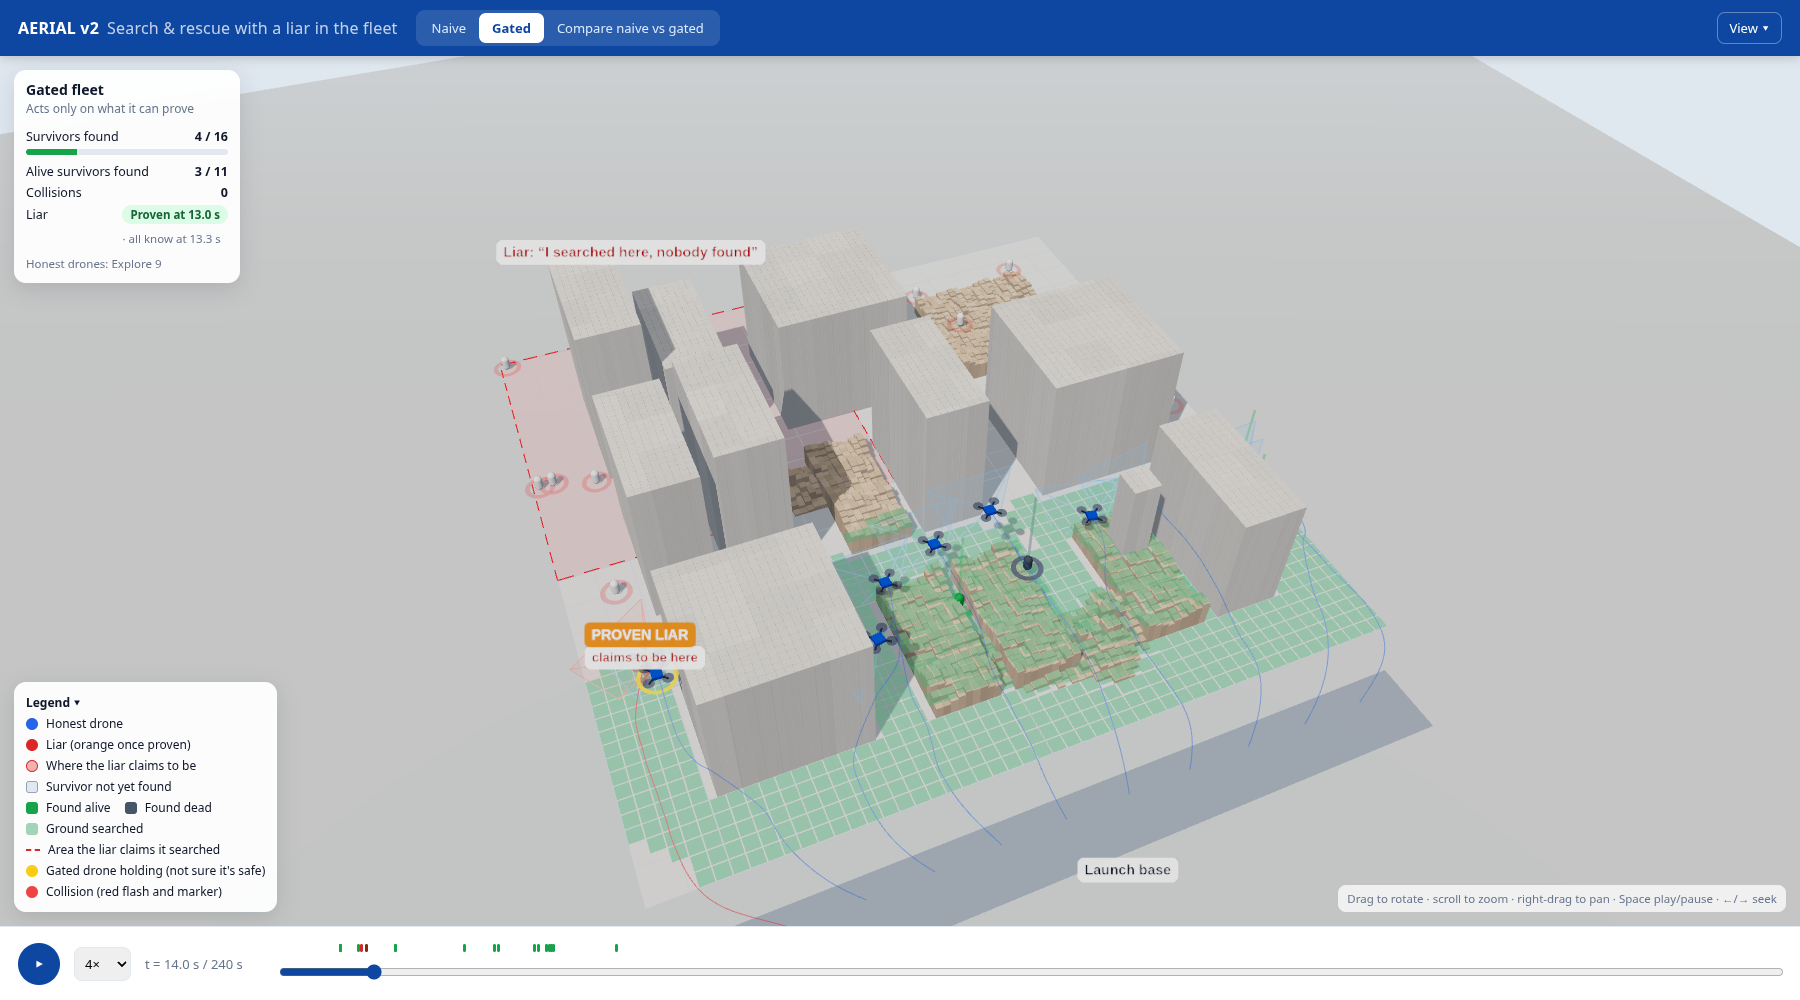
\includegraphics[width=\linewidth]{Figures/results/replay_caught.png}
    \caption[The liar is proven 0.8\,s after it starts lying]{Gated fleet at $t=14$\,s. The liar started lying at
    12.2\,s, claiming the dashed corner as searched while broadcasting a fake sweep over it (``claims to be here'').
    A neighbour compared the beacon with the UWB range of the same packet; the mismatch far exceeded $\varepsilon'$, so
    rule R1 fired at 13.0\,s. By 13.3\,s every honest drone knew the liar (orange label), and the corner had reopened
    for search.}
    \label{fig:demo-caught}
\end{figure}

\begin{figure}[!htbp]
    \centering
    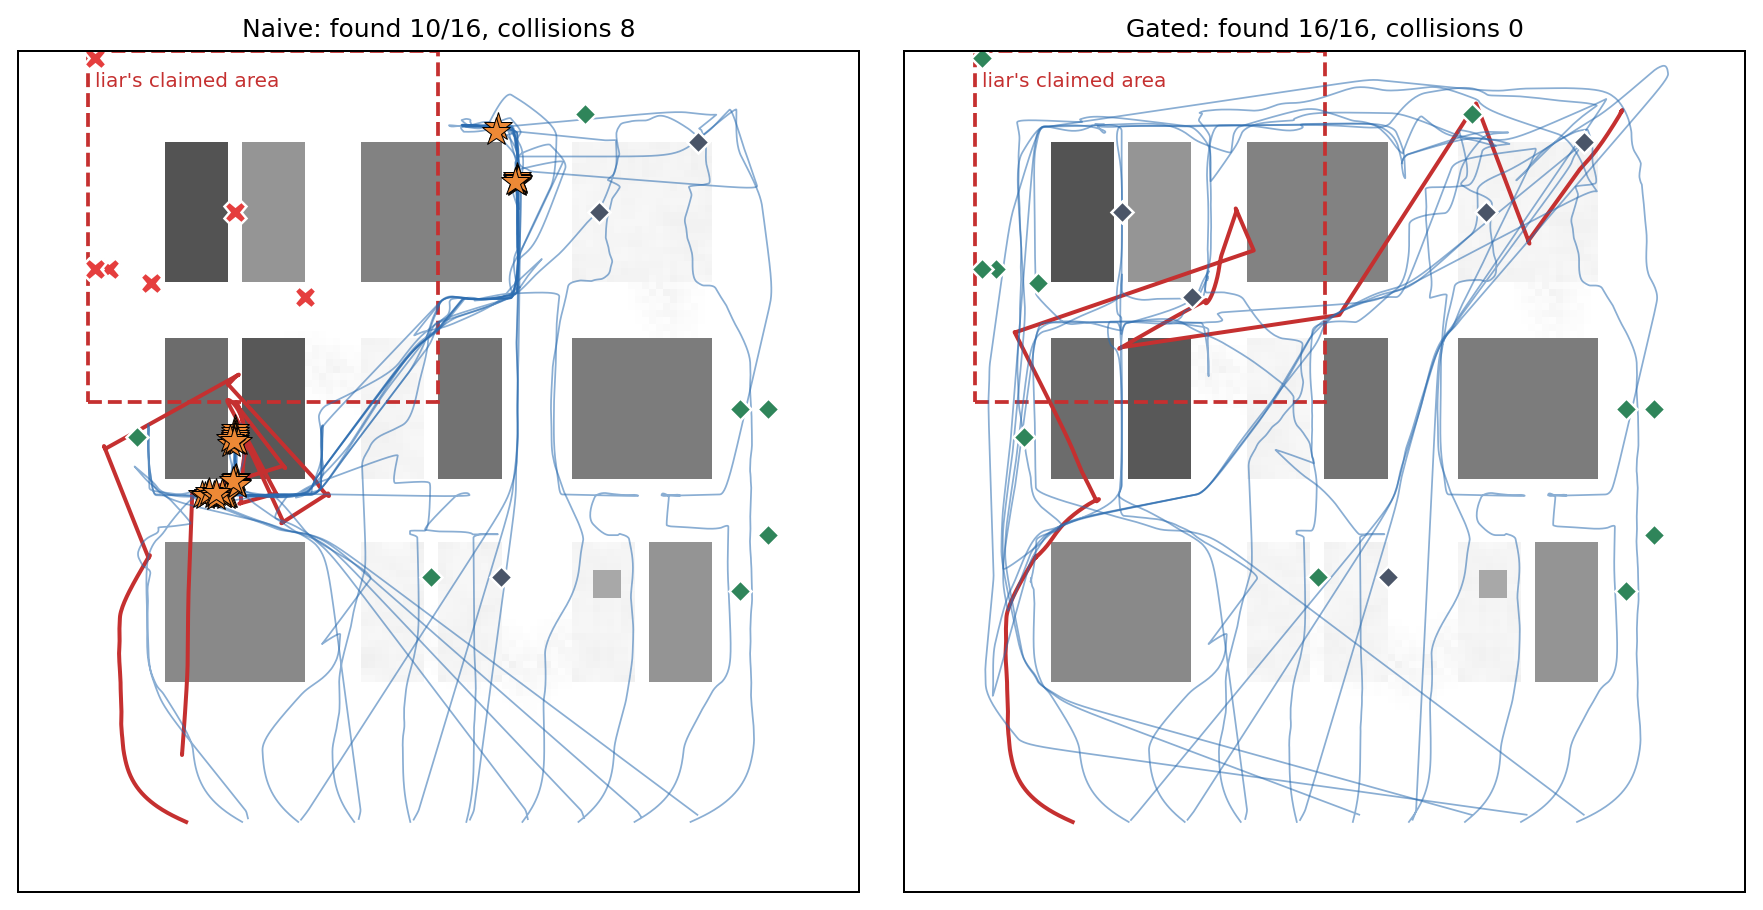
\includegraphics[width=\linewidth]{Figures/results/demo_topdown.png}
    \caption[Top-down trajectories of the demo mission]{Top-down view of the demo mission (blue: honest drones; red:
    the liar's true path). Green diamonds are survivors found alive, dark diamonds found dead, red crosses survivors
    never found, and stars are collisions. The naive fleet never enters the claimed corner and loses six survivors
    there. Its eight collisions are all between honest drones, which crowd into the remaining space without a motion
    gate. The gated fleet re-sweeps the corner and finds everyone.}
    \label{fig:demo-topdown}
\end{figure}

\begin{table}[!htbp]
\centering
\renewcommand{\arraystretch}{1.2}
\begin{tabular}{@{}l c c@{}}
\toprule
 & \naive{} & \gated{} \\
\midrule
Survivors found (alive found)          & 10/16 (7/11)  & \textbf{16/16 (11/11)} \\
Missed inside the liar's corner        & 6             & \textbf{0} \\
Collisions (pairs closer than 1\,m)    & 8 (all honest--honest) & \textbf{0} \\
First proof / all honest drones know the liar & never  & 13.0\,s / \textbf{13.3\,s} \\
All honest drones landed               & 188.9\,s      & 191.6\,s \\
False accusations                      & 0             & 0 \\
\bottomrule
\end{tabular}
\caption{The demo mission (one seed, demonstration liar).}
\label{tab:demo}
\end{table}

\autoref{fig:knowledge} makes the thesis visible. The naive fleet's \emph{believed} coverage jumps by about a quarter of
the zone the moment the liar's claim arrives; that jump is the ignorance. The gated fleet's \emph{known} coverage grows
only as fast as cells are really seen, and knowledge of the liar spreads to every honest drone within 1.1\,s of the lie.

\begin{figure}[!htbp]
    \centering
    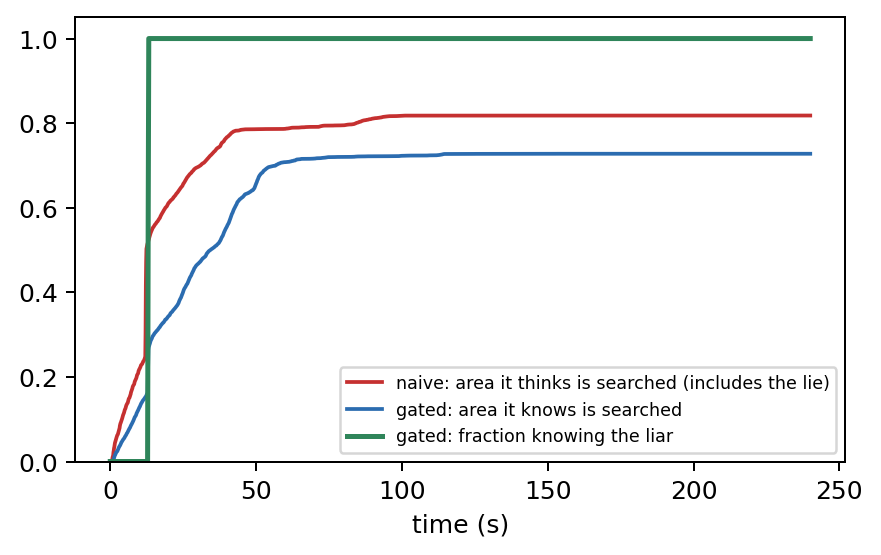
\includegraphics[width=0.72\linewidth]{Figures/results/knowledge_curves.png}
    \caption[Believed vs.\ known coverage, and knowledge of the liar]{Believed vs.\ known coverage in the demo mission
    (fractions of all 2,500 cells, including roofs that can never be searched). The step in the naive curve at 12\,s is
    the liar's false claim being accepted. The green curve is the fraction of honest gated drones that know who the
    liar is.}
    \label{fig:knowledge}
\end{figure}

\subsubsection{Parameter Sweep: Trust Costs Survivors}
\label{sec:res-sweep}

The sweep is our main experiment: 280 paired runs in which the naive fleet runs the same predictive gate as the gated
fleet but believes every report, so that \emph{trust is the only difference}. The results are in
\autoref{fig:sweep-found}, \autoref{fig:sweep-time} and \autoref{tab:sweep}.

\begin{figure}[!htbp]
    \centering
    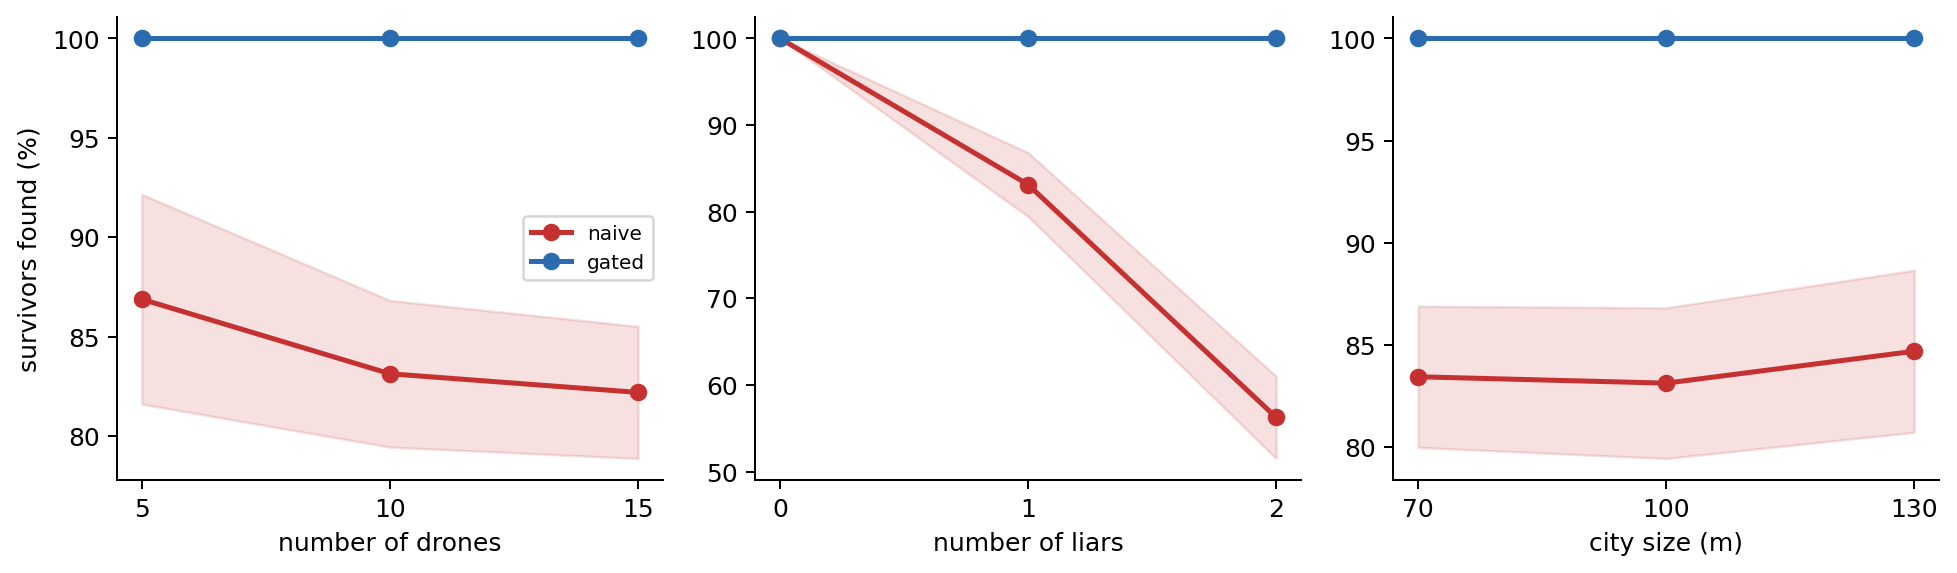
\includegraphics[width=\linewidth]{Figures/results/sweep_found.png}
    \caption[Sweep: survivors found]{Survivors found (mean of 20 paired seeds, 95\% interval shaded) when varying the
    number of drones, the number of liars, and the city size. The gated fleet finds every survivor in all 140 runs.}
    \label{fig:sweep-found}
\end{figure}

\begin{figure}[!htbp]
    \centering
    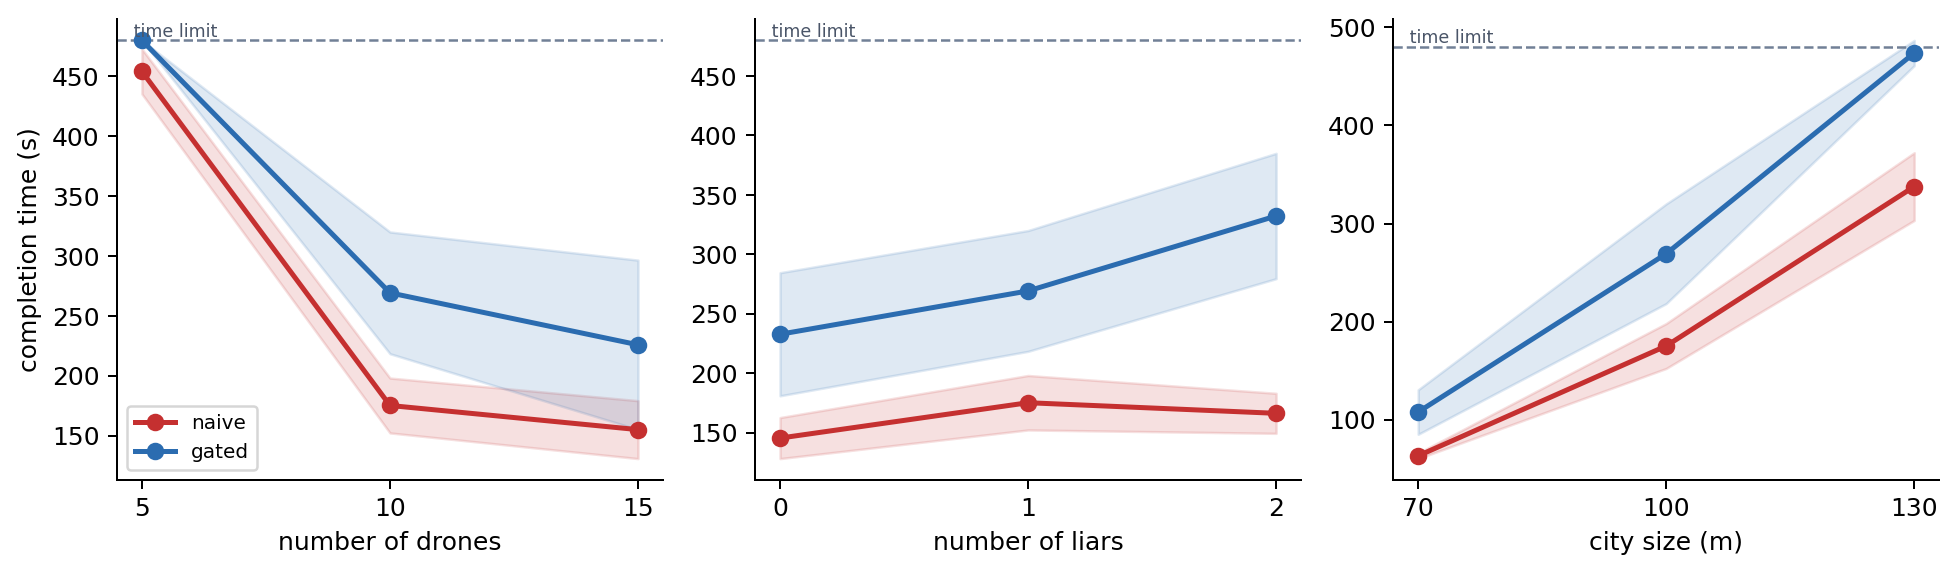
\includegraphics[width=\linewidth]{Figures/results/sweep_time.png}
    \caption[Sweep: completion time]{Completion time (all honest drones landed). Unfinished runs are scored at the
    480\,s limit (dashed), so the gated fleet's true cost with 5 drones or a 130\,m city is larger than shown.}
    \label{fig:sweep-time}
\end{figure}

\begin{table}[!htbp]
\centering
\renewcommand{\arraystretch}{1.18}
\begin{tabular}{@{}l l c c c c c c@{}}
\toprule
 & & \multicolumn{2}{c}{\textbf{Survivors found (\%)}} & \multicolumn{2}{c}{\textbf{Completion time (s)}} &
 \multicolumn{2}{c}{\textbf{Finished}} \\
\cmidrule(lr){3-4}\cmidrule(lr){5-6}\cmidrule(lr){7-8}
\textbf{Factor} & \textbf{Value} & naive & gated & naive & gated & naive & gated \\
\midrule
Drones   & 5           & $86.9\pm5.3$ & \textbf{100} & $454\pm19$ & $480\pm0$  & 50\%  & 0\% \\
         & 10 (base)   & $83.1\pm3.7$ & \textbf{100} & $175\pm23$ & $269\pm51$ & 100\% & 85\% \\
         & 15          & $82.2\pm3.3$ & \textbf{100} & $155\pm24$ & $226\pm71$ & 100\% & 80\% \\
\midrule
Liars    & 0           & 100          & 100          & $145\pm17$ & $233\pm52$ & 100\% & 95\% \\
         & 2           & $56.3\pm4.8$ & \textbf{100} & $166\pm17$ & $332\pm53$ & 100\% & 75\% \\
\midrule
City     & 70\,m       & $83.4\pm3.5$ & \textbf{100} & $63\pm3$   & $108\pm23$ & 100\% & 100\% \\
         & 130\,m      & $84.7\pm4.0$ & \textbf{100} & $338\pm35$ & $474\pm13$ & 90\%  & 5\% \\
\bottomrule
\end{tabular}
\caption[Sweep results]{Sweep results, mean $\pm$ 95\% interval over 20 paired seeds. The naive--gated difference
in survivors found is significant wherever a liar is present (Wilcoxon $p<0.002$ in every setting). The worst naive
run found 69\% of survivors with one liar and 44\% with two.}
\label{tab:sweep}
\end{table}

\begin{findingbox}[Finding 1: trust costs survivors, not collisions]
With one liar the naive fleet misses about one survivor in six in \emph{every} setting, essentially regardless of fleet
size or city size. With two liars it loses almost half. The gated fleet loses \emph{nobody} in 140 runs. Once both
fleets share the predictive safety check, collisions are rare and equal: 3 in 280 runs (two involving a liar in gated
runs, one in a naive run), with no significant difference ($p\ge0.32$; \autoref{fig:sweep-collisions}).
\end{findingbox}

\begin{figure}[!htbp]
    \centering
    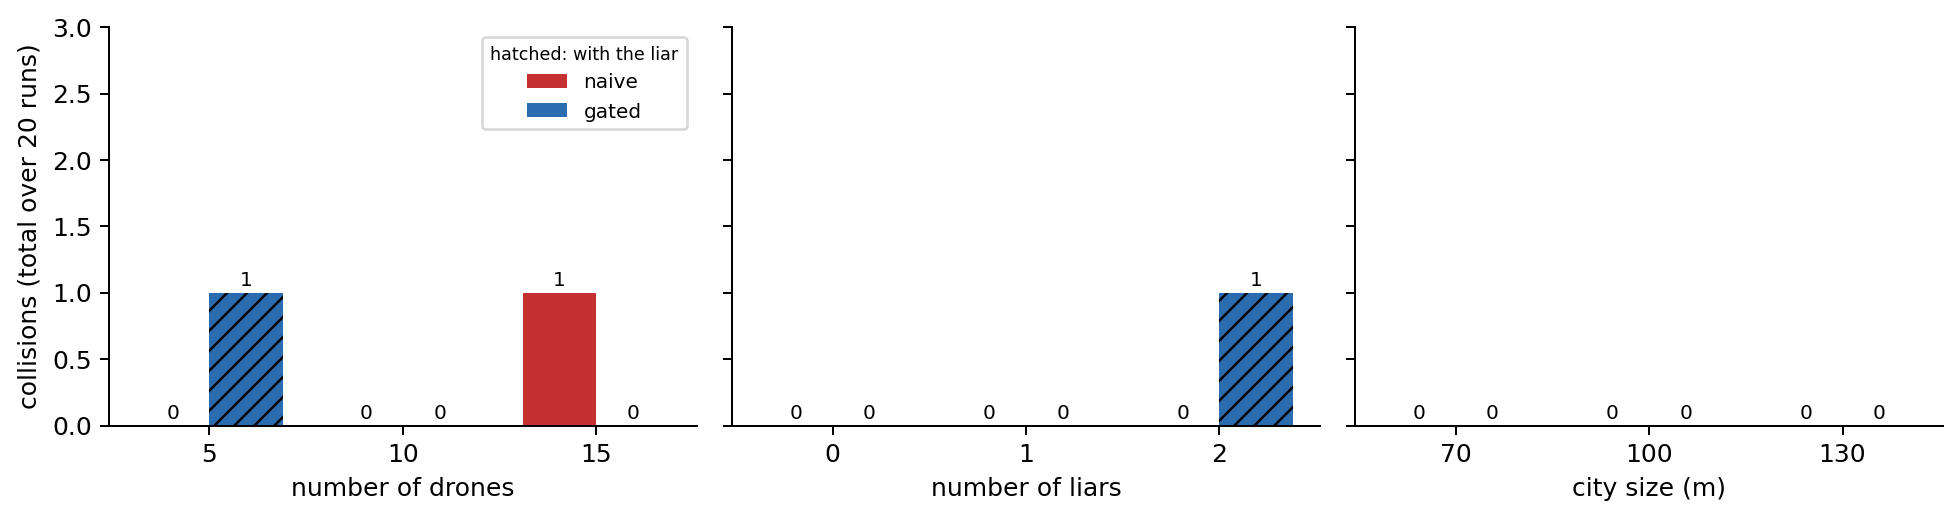
\includegraphics[width=\linewidth]{Figures/results/sweep_collisions.png}
    \caption{Sweep: collisions, totalled over 20 runs per setting (hatched: involving the liar).}
    \label{fig:sweep-collisions}
\end{figure}

\textbf{The cost of caution.} The gated fleet pays in time, about $+90$\,s at the baseline (269 vs.\ 175\,s,
$p=0.002$). Most of it is paid \emph{even with no liar} ($+87$\,s, $p<0.001$): it is the price of \emph{caution}
(holding when a move cannot be proven safe, flying only through space seen by itself or a known-honest teammate, and
auditing), not of uncertainty about who the liar is. The cost grows with
the work per drone: with 5 drones or a 130\,m city the gated fleet rarely finishes within 480\,s, while with 15 drones
the time gap is no longer significant ($p=0.19$). \autoref{fig:sweep-tradeoff} summarises the trade-off: every arrow
goes from the naive to the gated fleet on the same setup, always up (more survivors) and to the right (more time).

\begin{figure}[!htbp]
    \centering
    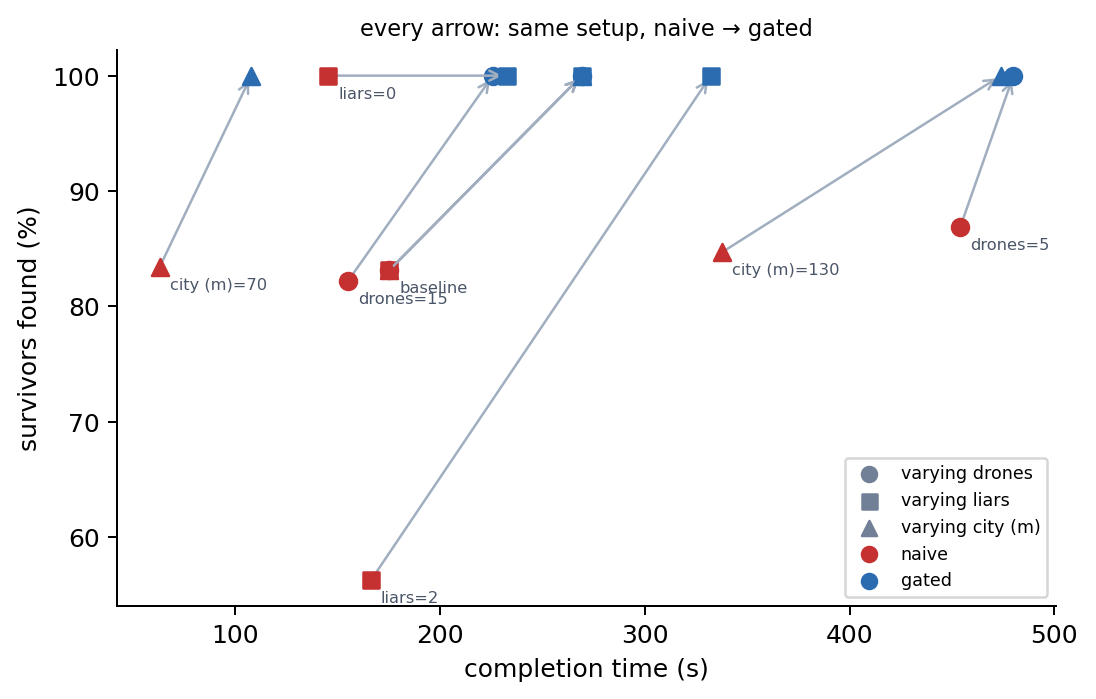
\includegraphics[width=0.78\linewidth]{Figures/results/sweep_tradeoff.png}
    \caption[The trade-off: survivors vs.\ time]{The trade-off. Each arrow joins the naive (red) and gated (blue)
    fleet on the same setting. Only the no-liar setting starts at 100\%.}
    \label{fig:sweep-tradeoff}
\end{figure}

\textbf{Identifying the liar.} The liar was identified in all 120 gated runs that contained one, with \textbf{no false
accusation} in any run. The first proof came a median 0.7--6.7\,s after the lie started, depending on the setting
(\autoref{tab:detection}). The range check R1 fired first in 76 runs, the speed check R2 in 32, an audit (R5) in 9 and the
camera (R4) in 3. In most settings every honest drone knew the liar within a fraction of a second of the first proof:
corroborating evidence spreads as fast as gossip. With only 5 drones, or 15 drones spread thinly, the second
independent proof that Corollary~\ref{cor:framing} requires takes longer to appear.

\begin{table}[!htbp]
\centering
\renewcommand{\arraystretch}{1.18}
\begin{tabular}{@{}l c c c c c c@{}}
\toprule
 & 5 drones & base & 15 drones & 2 liars & 70\,m & 130\,m \\
\midrule
Liar caught (gated)       & 20/20 & 20/20 & 20/20 & 20/20 & 20/20 & 20/20 \\
First proof (median, s)   & 12.9  & 14.6  & 18.9  & 14.4  & 15.5  & 13.1 \\
All honest know (median, s) & 38.6 & 14.8 & 24.6  & 14.7  & 15.7  & 13.8 \\
First rule (R1/R2/R4/R5)  & 15/5/0/0 & 13/7/0/0 & 13/2/2/3 & 10/10/0/0 & 10/3/1/6 & 15/5/0/0 \\
\bottomrule
\end{tabular}
\caption[Sweep: liar identification]{Liar identification in the sweep (the liar starts lying at 12.2\,s). In the
two-liar setting, ``caught'' means at least one liar proven. Zero false accusations in all 280 runs.}
\label{tab:detection}
\end{table}

\subsubsection{Four Fleets: Is the Price in \emph{Who} or in \emph{Where}?}
\label{sec:res-e1}

E1 adds the two reference fleets on 30 new districts, with the fair gate for every fleet (\autoref{fig:e1}).

\begin{figure}[!htbp]
    \centering
    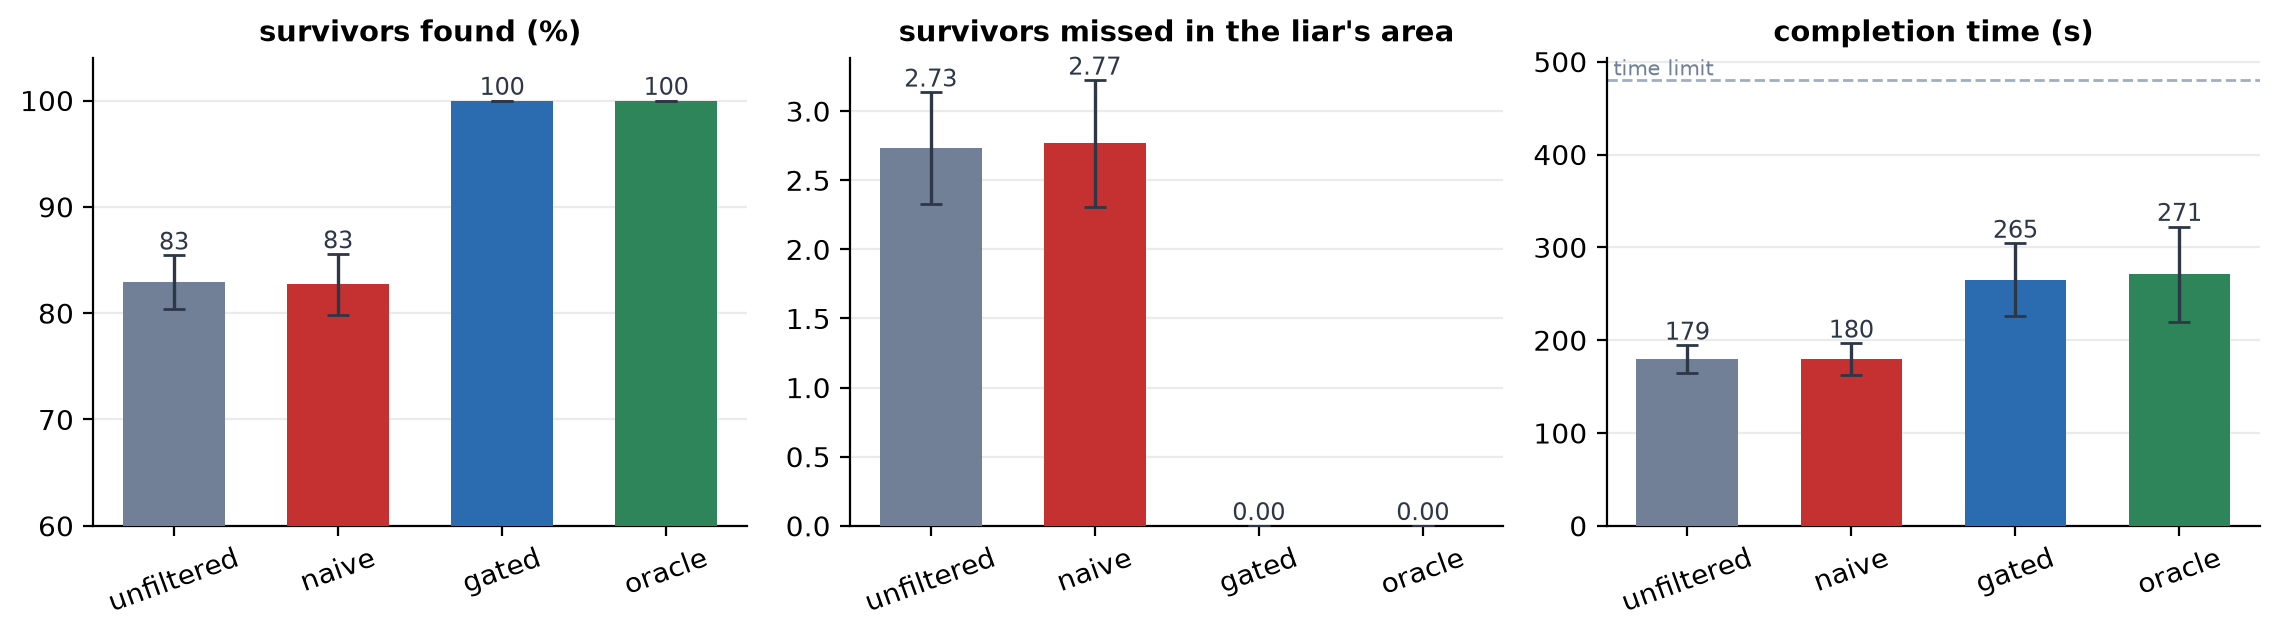
\includegraphics[width=\linewidth]{Figures/results/report_e1_fleets.png}
    \caption[E1: four fleets on 30 districts]{E1: the four fleets on 30 paired districts with one range-aware liar
    (95\% intervals). There were no collisions in any of the 120 runs.}
    \label{fig:e1}
\end{figure}

\begin{findingbox}[Finding 2: filtering alone buys nothing in the search, and the price of caution is not ignorance of the liar's identity]
\begin{itemize}
    \item \textbf{W-MSR does not help the search.} The naive fleet ($82.7\pm2.9\%$ found) is indistinguishable from
          the completely unfiltered fleet ($82.9\pm2.5\%$). Both miss survivors in all 30 districts, on average
          2.8 inside the liar's corner, because the damaging lie is a claim, and claims cannot be filtered.
    \item \textbf{Knowing beats filtering.} The gated fleet finds 100\% in all 30 districts ($p=1.5\times10^{-6}$ vs.\ naive)
          and knows the liar within $15.9\pm1.3$\,s.
    \item \textbf{The gated fleet matches the oracle.} The oracle, told the liar at $t=0$, is \emph{no faster}
          (271 vs.\ 265\,s, $p=0.94$). The time the gated fleet spends is spent on caution about \emph{where} drones may
          be, not on finding out \emph{who} lies. Once the liar is known, the gated fleet behaves exactly like the oracle.
\end{itemize}
\end{findingbox}

\subsubsection{Which Liars are Caught? (E2)}
\label{sec:res-e2}

E2 varies the kind of lie: three ways of faking a position (\emph{fake sweep}, a blunt fake trajectory over the corner;
\emph{range-aware}, which matches every listener's range where geometry allows; \emph{radio shadow}) and a liar that
flies its \emph{true} position and lies only about coverage. Each is crossed with two ways of claiming: the whole
corner at once, or cell by cell as its (fake) sweep passes. The results are in \autoref{fig:e2} and
\autoref{tab:e2}.

\begin{figure}[!htbp]
    \centering
    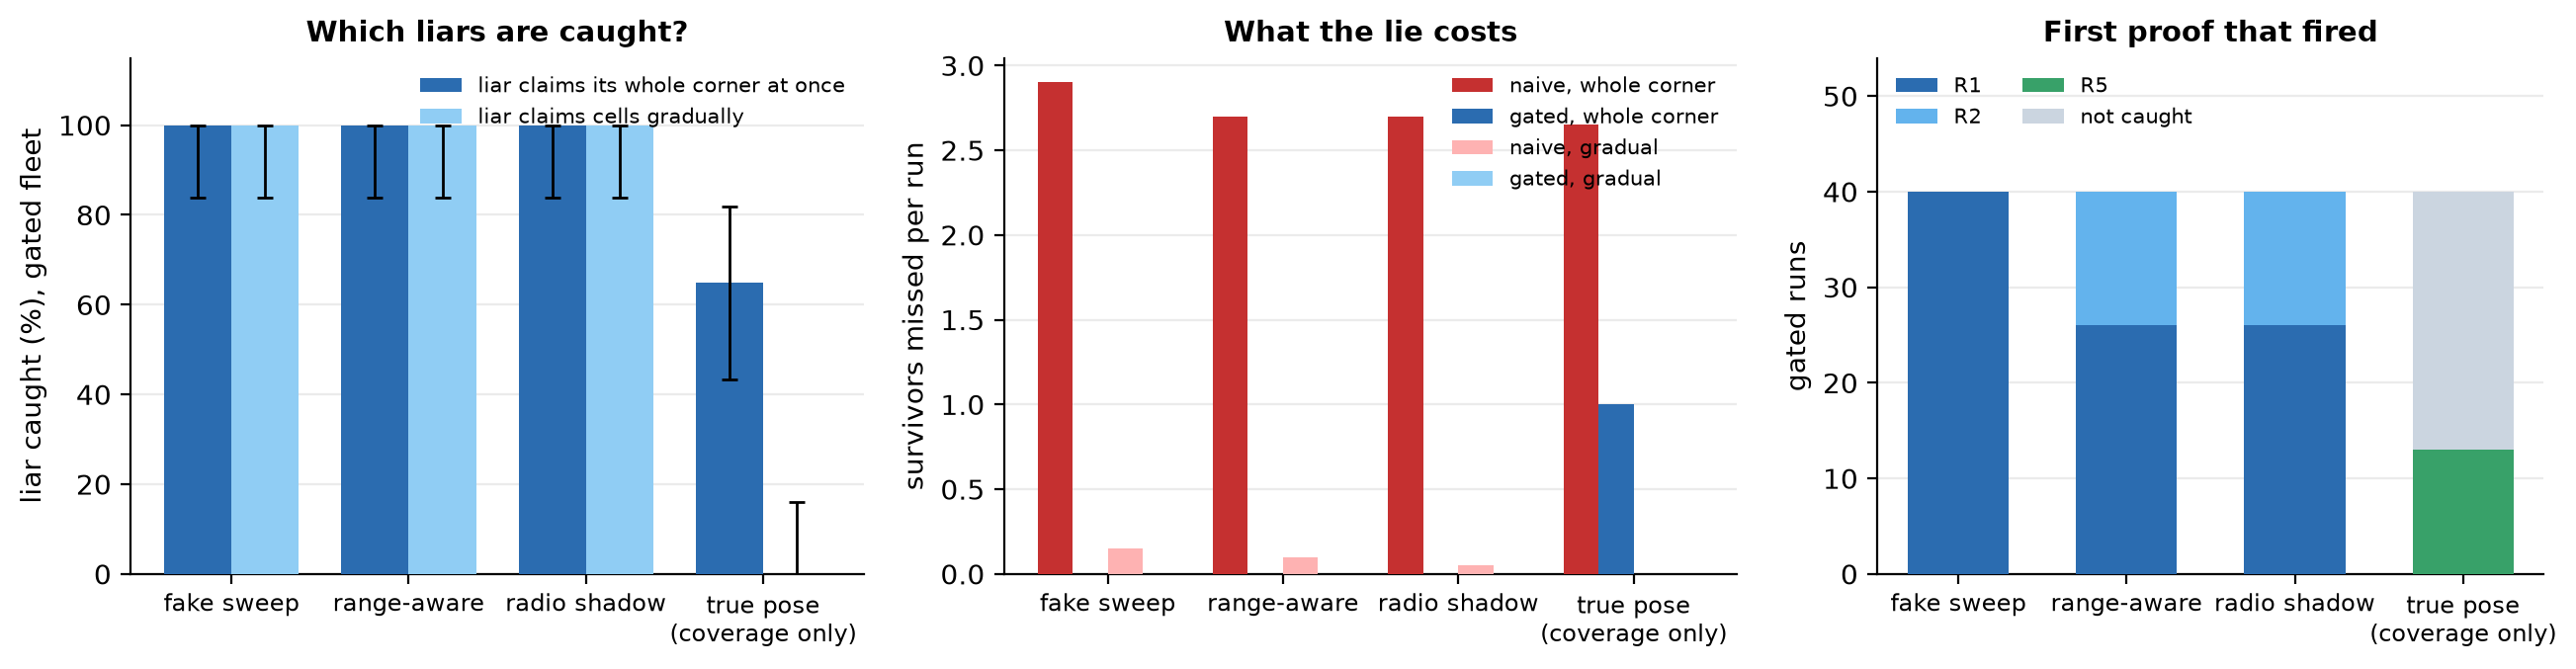
\includegraphics[width=\linewidth]{Figures/results/report_e2_detection.png}
    \caption[E2: detection by liar type]{E2: catch rate of the gated fleet with 95\% Wilson intervals (left), survivors
    missed per run (middle; bars at zero are not drawn), and the first proof that identified the liar (right; 40
    gated runs per liar type).}
    \label{fig:e2}
\end{figure}

\begin{table}[!htbp]
\centering
\renewcommand{\arraystretch}{1.18}
\begin{tabular}{@{}l l c c c c@{}}
\toprule
\textbf{Position lie} & \textbf{Claims} & \textbf{Caught} & \textbf{First proof / all know (s)} &
\multicolumn{2}{c}{\textbf{Survivors found (\%)}} \\
\cmidrule(lr){5-6}
 & & (gated) & (median) & naive & gated \\
\midrule
fake sweep   & whole corner & 20/20 & 12.3 / 12.5 & 81.9 & \textbf{100} \\
             & gradual      & 20/20 & 12.3 / 12.5 & 99.1 & \textbf{100} \\
range-aware  & whole corner & 20/20 & 14.6 / 14.8 & 83.1 & \textbf{100} \\
             & gradual      & 20/20 & 14.6 / 14.8 & 99.4 & \textbf{100} \\
radio shadow & whole corner & 20/20 & 14.7 / 14.9 & 83.1 & \textbf{100} \\
             & gradual      & 20/20 & 14.7 / 14.9 & 99.7 & \textbf{100} \\
true pose (coverage only) & whole corner & 13/20 & 33.1 / 44.1 & 83.4 & 93.8 \\
             & gradual      & 0/20  & -- & 100 & 100 \\
\bottomrule
\end{tabular}
\caption[E2: detection results]{E2 results (20 paired seeds per row; lying starts at 12.2\,s). No false
accusation occurred in any of the 320 runs.}
\label{tab:e2}
\end{table}

\begin{findingbox}[Finding 3: a position lie is caught at once; a pure coverage lie only by audits]
\begin{itemize}
    \item \textbf{Every liar that fakes its position is caught}, in 120 of 120 runs, a median 0.1--2.5\,s after it
          starts lying. Even the range-aware liar cannot hide: whenever three listeners surround it, or it moves faster
          than a drone can fly to keep its story consistent, R1 or R2 fires.
    \item \textbf{The damage comes from claiming a large area.} A liar that claims its whole corner costs the naive
          fleet 2.7--2.9 survivors per run. A liar that claims cells only along its fake path costs almost nothing
          (0.05--0.15), because overlapping honest cameras re-view most of those cells anyway.
    \item \textbf{A coverage-only liar is the hard case.} It is caught only by an audit (R5), in 13 of 20 runs, a
          median 21\,s after the lie. Whenever it was caught, the gated fleet found everyone. In the 7 runs where the
          audits missed it, the gated fleet lost 1--5 survivors, as many as the naive fleet. When the same liar claims
          gradually it is never caught, but it is then also harmless: both fleets found every survivor.
\end{itemize}
\end{findingbox}

\textbf{A safety weakness exposed by E2.} All 22 collisions of E2 occurred against the blunt \emph{fake sweep} liar,
which hovers in place while claiming to be far away: 16 in 12 of 40 gated runs, and 6 in 5 of 40 naive runs. No other
liar type caused any. Two affected gated runs, re-flown with full logging, reproduced exactly: every collision was an
honest gated drone touching the hovering liar, 70--85\,s after the liar had been proven. A proven liar's beacons no
longer count as positions, and the range-shell check that replaces them probes only along the direction of motion
(\autoref{sec:limitations}), so a drone re-sweeping the reopened corner can drift into a liar it has not just sighted.
The range-aware liar is unaffected because its claimed position stays close to its real one. Checking the whole
reachable shell, as in the extended gate of \autoref{sec:res-collision}, is the clearest target for future work.

\subsubsection{The Caution Knob: Audit Fraction (E3)}
\label{sec:res-e3}

E3 targets the hardest case from E2, the coverage-only liar that claims its whole corner, and varies the audit
fraction $q$ over 30 districts (\autoref{fig:e3}).

\begin{figure}[!htbp]
    \centering
    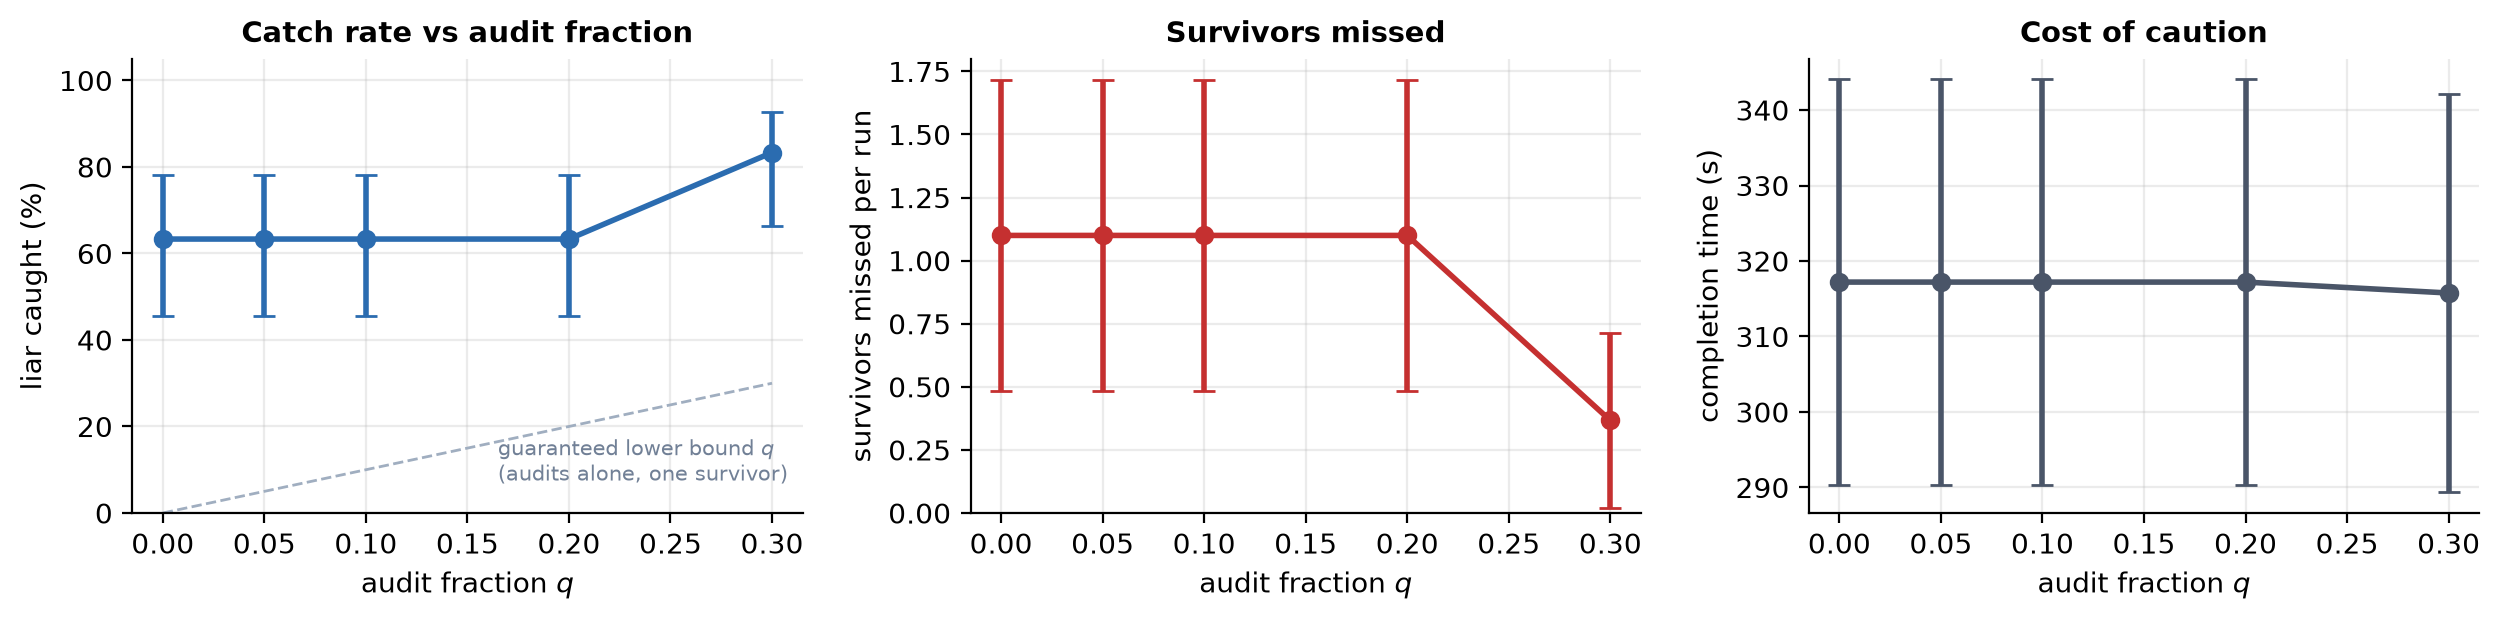
\includegraphics[width=\linewidth]{Figures/results/report_e3_audit.png}
    \caption[E3: the audit fraction]{E3: catch rate (95\% Wilson intervals), survivors missed and completion time against
    the audit fraction $q$, for a liar that flies its true position and lies only about coverage (30 paired districts
    per value). The dashed line is the guarantee of Proposition~\ref{prop:audit} for deliberate audits alone. Only
    9--11 of 30 runs per value finished within the 360\,s limit, so the time panel cannot resolve the cost of $q$.}
    \label{fig:e3}
\end{figure}

\begin{findingbox}[Finding 4: overlapping cameras audit for free; deliberate audits matter only above that level]
\begin{itemize}
    \item With $q=0$, i.e.\ no deliberate audits at all, the liar is still caught in 63\% of runs (19/30). Honest
          drones' cameras overlap at region borders and incidentally view cells the liar claimed. A survivor seen in
          such a cell is a proof (R5), whoever looked.
    \item Up to $q=0.2$ nothing changes. The audit budget $\lceil q\,n_j\rceil$ is already met by those incidental
          views, so no extra cell is visited, and the 30 runs come out identical for every $q\le0.2$.
    \item At $q=0.3$ the budget exceeds the free overlap. The catch rate rises to 83\% (25/30), and survivors missed
          fall from $1.10\pm0.62$ to $0.37\pm0.35$ per run. The measured catch rates stay well above the guaranteed lower
          bound of Proposition~\ref{prop:audit}.
\end{itemize}
\end{findingbox}

The practical lesson is that $q$ should be set relative to the \emph{free} audit rate of the fleet geometry. Below it,
audits cost nothing and add nothing. Above it, every extra percent of audits buys a measurable increase in the chance
of exposing a coverage-only liar.

\subsubsection{A Liar Hiding in the Flight Path}
\label{sec:res-collision}

The quantitative experiments use a passive liar. To illustrate the safety side of the gate, we also recorded a stress
demonstration: the liar claims to sweep its far corner while waiting, still, in the path of honest drones, 0.6\,m above
the height the camera covers. This liar and the extended gate (which checks the whole reachable cone of the range shell)
are an experimental extension outside the evaluated code, so the replay is an illustration only
(\autoref{fig:collision}). The naive fleet, believing the fake position, flew into the liar six times and missed three
survivors. The gated fleet, treating a possible liar as ``somewhere on its range sphere'', had no collision, knew the
liar by 12.5\,s and found all 16 survivors, at the price of a longer mission (365 vs.\ 212\,s).

\begin{figure}[!htbp]
    \centering
    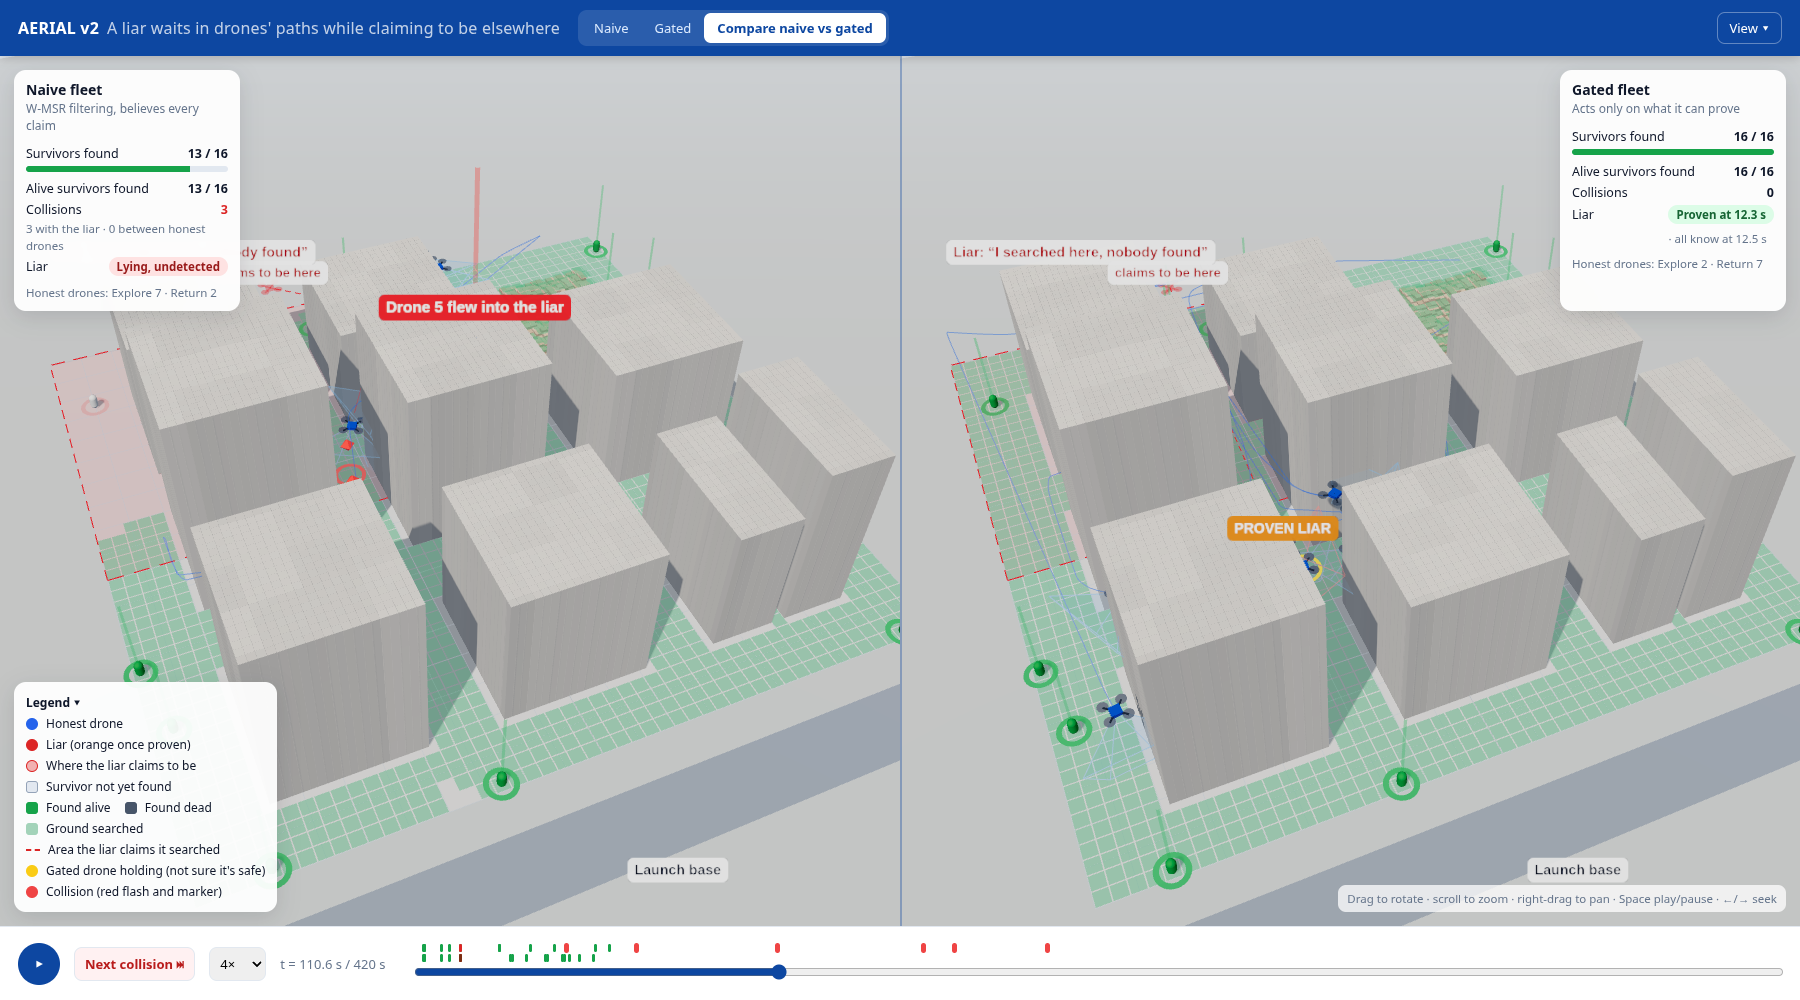
\includegraphics[width=\linewidth]{Figures/results/replay_collision.png}
    \caption[Illustration: naive drones fly into a hidden liar]{Illustration (experimental liar extension): at
    110.6\,s a naive drone flies into the liar (left), which it believes to be elsewhere. The gated drones keep their
    distance from the liar's range sphere and from its camera-located position (right).}
    \label{fig:collision}
\end{figure}

\subsubsection{Resilient Survivor Localisation}
\label{sec:res-localisation}

Where numbers \emph{are} involved, W-MSR does its job (\autoref{fig:localisation}). When one of 2--8 observers reports a
survivor's position offset by up to 20\,m, the plain mean is dragged by almost the full lie (19.8\,m of a 20\,m lie with
5 observers). W-MSR stays within 0.2--0.7\,m of the truth for every lie size. The price appears when nobody lies: W-MSR
discards honest data and has 0.2--0.45\,m error, against almost zero for the mean.

\begin{figure}[!htbp]
    \centering
    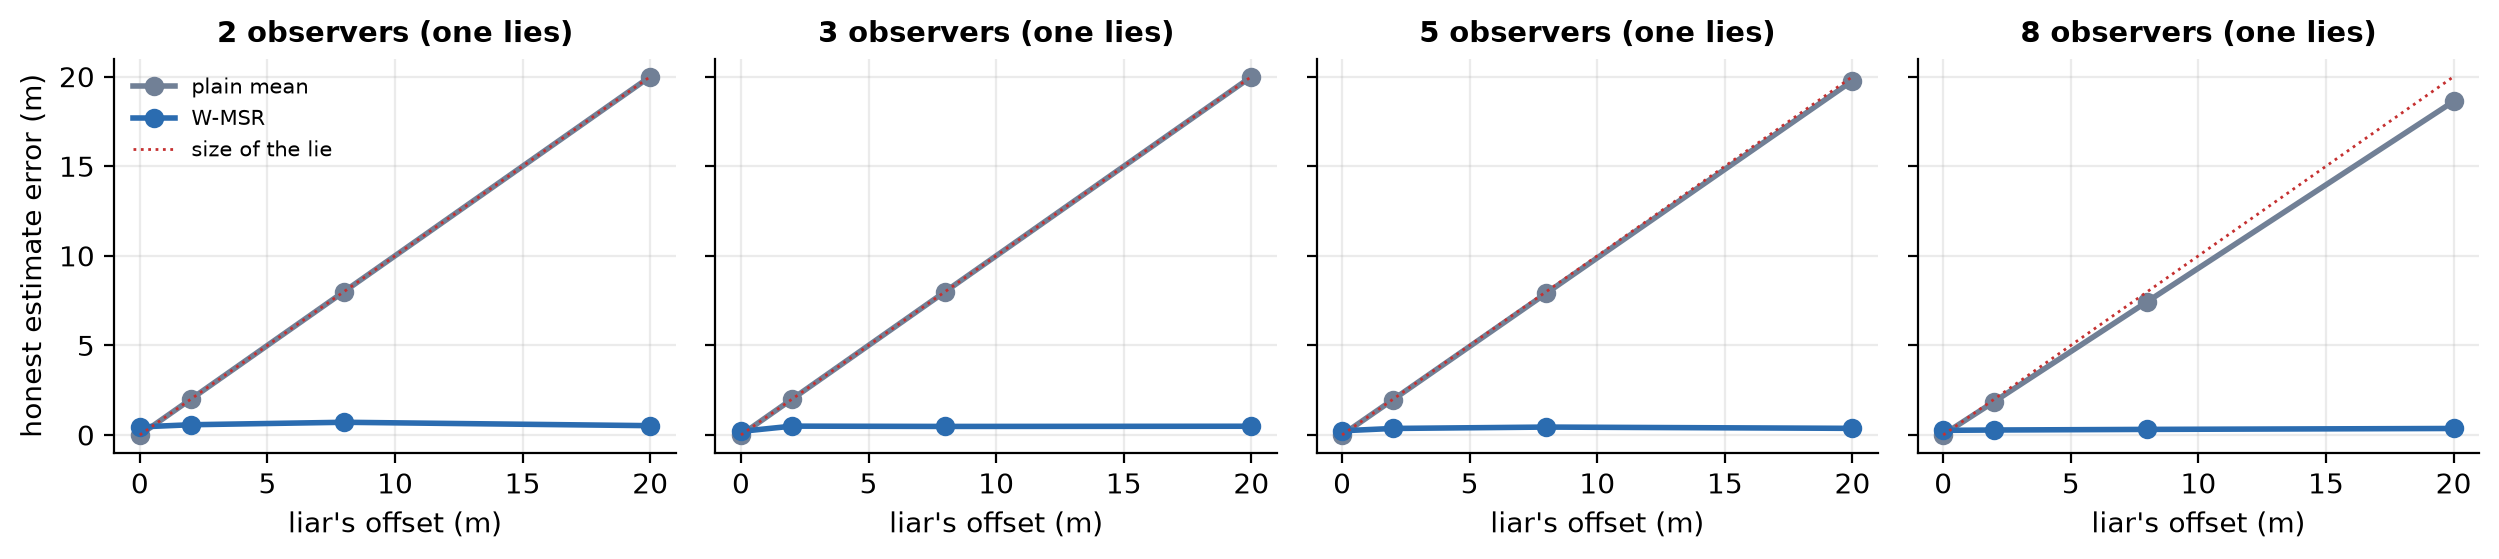
\includegraphics[width=\linewidth]{Figures/results/report_localisation.png}
    \caption[Survivor localisation: W-MSR vs.\ mean]{Error of the honest drones' combined estimate of a survivor's
    position when one observer lies by a given offset.}
    \label{fig:localisation}
\end{figure}

\subsubsection{Theory Studies from the 2D Build}
\label{sec:res-theory}

A first, simpler 2D build of the project (fixed-topology formation flight) was used to check the network theory behind
the fleet. Its studies (\autoref{fig:lambda2}, \autoref{fig:er}, \autoref{fig:degradation}) support three statements
used in the main system:

\begin{enumerate}
    \item \textbf{Algebraic connectivity predicts convergence} (480 runs). The convergence rate grows with $\lambda_2$
          and then saturates at the limit set by the controller gains. Predicted from the whole Laplacian spectrum, it
          is accurate to within 1.7\% mean error without packet loss. Under 30\% packet loss, using $\lambda_2$ alone
          gives 70\% error, so the full spectrum is needed.
    \item \textbf{$(2F+1)$-robustness is sufficient, not necessary} (4,860 runs on Erd\H{o}s--R\'enyi graphs). When the
          condition held, W-MSR succeeded in all 1,428 runs with $F=1$. When it failed, only 32\% of 1,002 runs
          succeeded, and the unfiltered mean succeeded in 5\% overall.
    \item \textbf{W-MSR collapses as soon as liars exceed $F$, and costs information when nobody lies.} Success is
          100\% while the actual number of liars is at most the assumed $F$, then falls sharply. With nobody lying,
          W-MSR discards 29\% ($F=1$) and 51\% ($F=2$) of honest messages.
\end{enumerate}

A 14,400-run trade-off study in the same build (four attacks, packet loss, gate horizon and margin) found the same
pattern as the 3D sweep. The gated fleet violated the STL safety requirement in 1.5\% of runs, against 99.9\% for the
naive fleet. The oracle fleet gained nothing over the gated fleet, again because the price is where the liar might be,
not who it is.

\begin{figure}[!htbp]
    \centering
    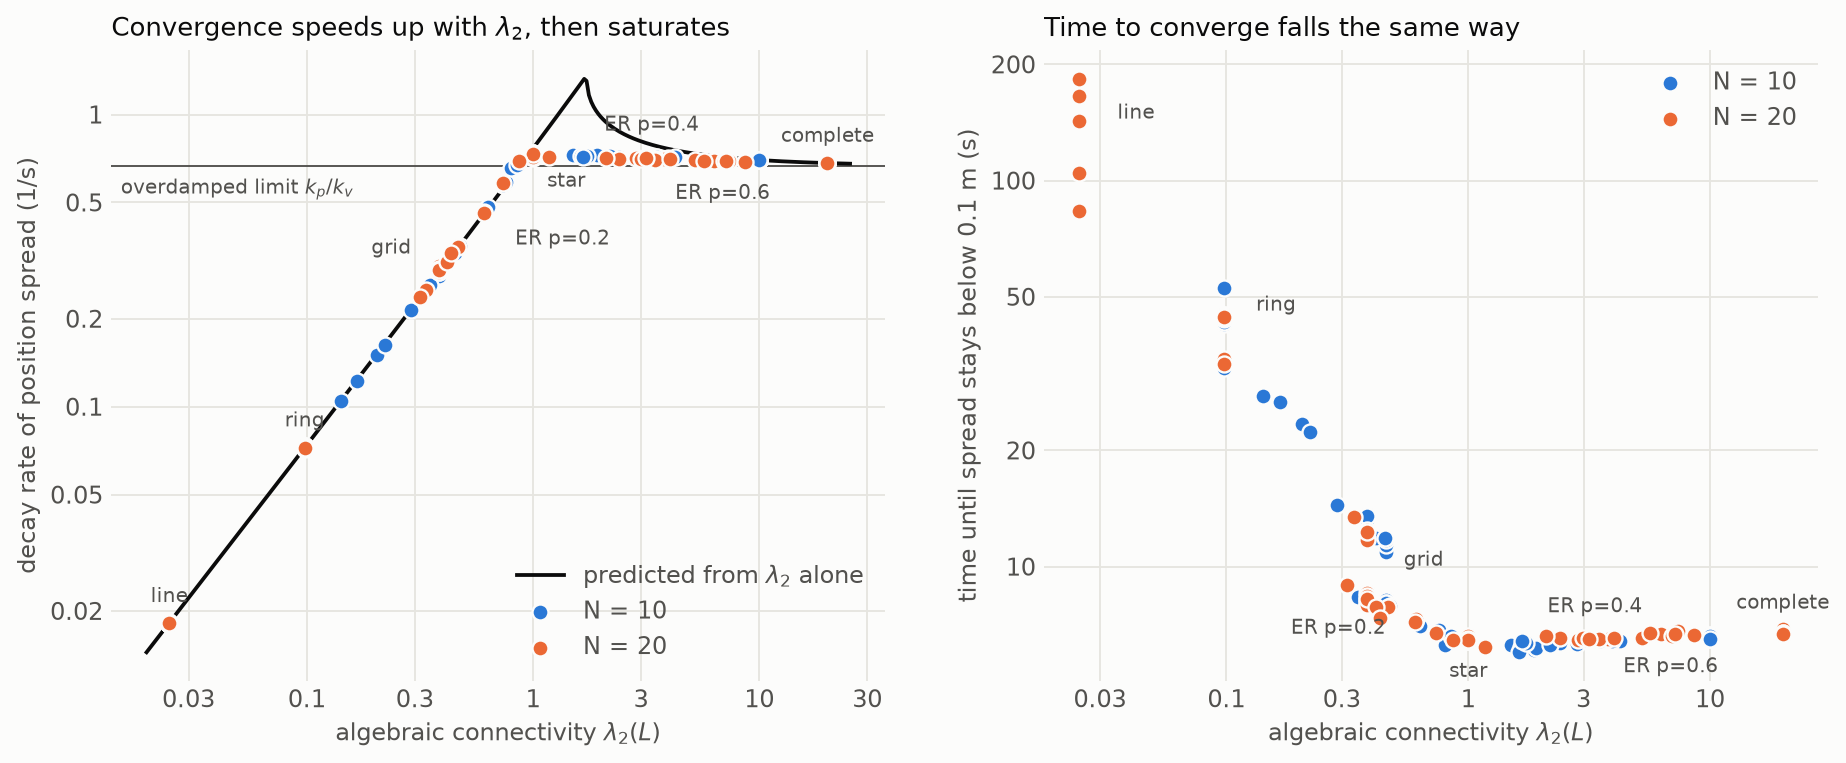
\includegraphics[width=\linewidth]{Figures/results/lambda2_convergence.png}
    \caption[2D study: convergence vs.\ algebraic connectivity]{2D study: consensus convergence rate (left) and time
    to converge (right) against the algebraic connectivity $\lambda_2$, for six topologies and Erd\H{o}s--R\'enyi graphs.}
    \label{fig:lambda2}
\end{figure}

\begin{figure}[!htbp]
    \centering
    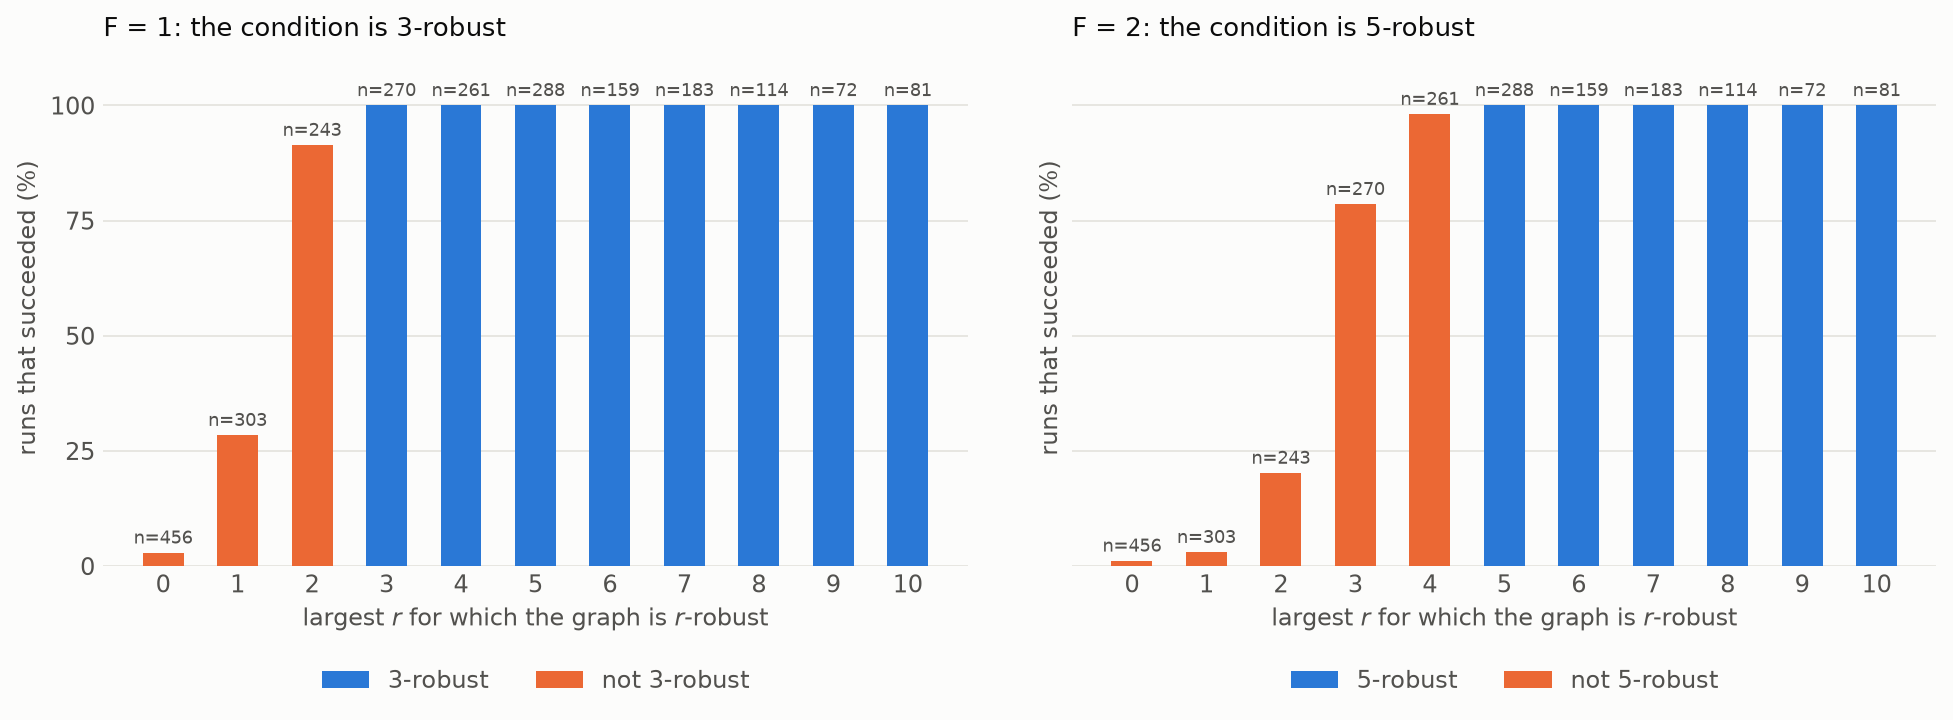
\includegraphics[width=\linewidth]{Figures/results/er_robustness.png}
    \caption[2D study: W-MSR success vs.\ network robustness]{2D study: W-MSR success on Erd\H{o}s--R\'enyi graphs
    against the graph's robustness (blue: the sufficient condition holds).}
    \label{fig:er}
\end{figure}

\begin{figure}[!htbp]
    \centering
    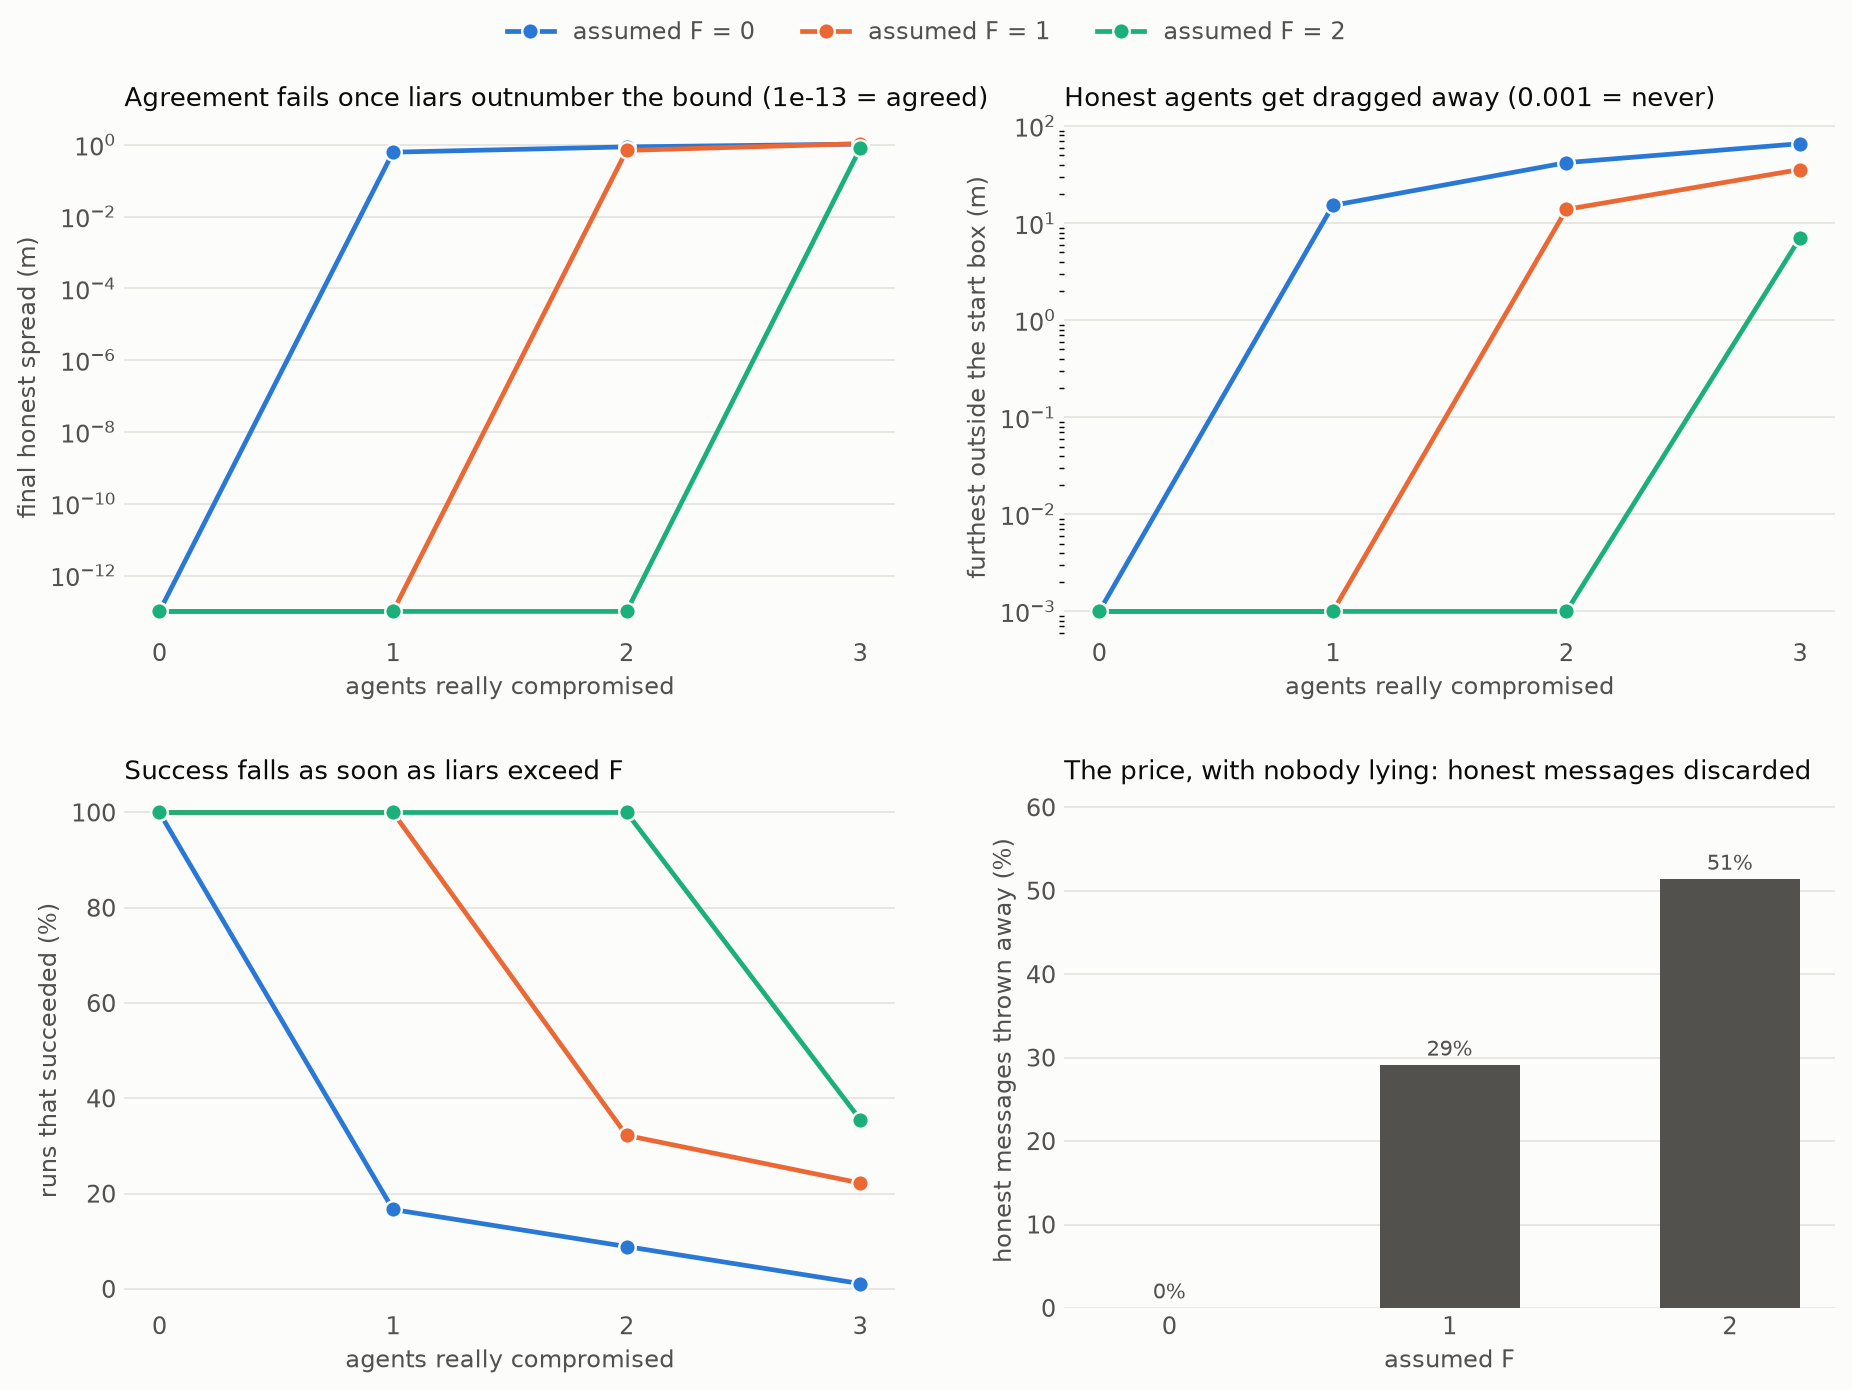
\includegraphics[width=0.85\linewidth]{Figures/results/degradation.png}
    \caption[2D study: graceful degradation of W-MSR]{2D study: what happens when the actual number of liars exceeds
    the assumed $F$ (top, bottom left), and the information W-MSR throws away when nobody lies (bottom right).}
    \label{fig:degradation}
\end{figure}

\FloatBarrier
\section{Limitations}
\label{sec:limitations}

Each limitation below bounds what the results above can claim.

\textbf{Performance.}
\begin{itemize}
    \item \textbf{Caution costs time}: about $+90$\,s at the baseline, \emph{even with no liar}. With a small fleet or
          a large city, the gated fleet often does not finish within 480\,s, so its true time there is underestimated.
    \item \textbf{Coverage-only liars are caught only by audits}, and audits are probabilistic
          (Proposition~\ref{prop:audit}); see E2 and E3.
\end{itemize}

\textbf{Model.}
\begin{itemize}
    \item Signed messages without equivocation, range noise bounded by 0.2\,m (real UWB has rare outliers, which would
          require a robust version of R1), static 2.5D terrain without overhangs, point drones, and no wind.
    \item \textbf{Terrain contact.} Drones are points and the terrain is a 1\,m raster. In the sweep, honest drones of
          both fleets occasionally grazed a wall: a 1\,Hz trajectory sample fell inside a building's outermost 1\,m
          cell in 56 of 140 naive and 69 of 140 gated runs. In 97\% of these cases the drone was at most 1\,m inside
          and only for a single sample (the worst case was 5\,m). These contacts are excluded from the collision
          counts, which count drone pairs only. A body radius and a terrain term in the gate would remove them.
    \item A liar that deliberately rams other drones (Assumption A8) defeats any gate that controls only the honest
          drone's own motion. This is out of scope.
\end{itemize}

\textbf{Method.}
\begin{itemize}
    \item The gate's check against a possible liar's range shell is analytic and probes only along the direction of
          motion. Against a hovering liar that claims to be far away, this let gated drones touch the liar in 12 of 40
          E2 runs (\autoref{sec:res-e2}). A possible liar whose latest packet was lost is covered only by the silence
          rule.
    \item ``Done'' uses belief plus audits. The fraction of \emph{known}-cleared cells is reported but not required for
          landing.
    \item Planned but not built: a rule R7 for coverage claims that are impossible from the liar's true path,
          heading-based altitude layers (layers are assigned by drone id), a consensus-based regroup at the base, and
          full 3D detours.
\end{itemize}

\textbf{Evaluation.}
\begin{itemize}
    \item All results are from simulation, with 20--30 seeds per configuration. The demonstrations use one seed each,
          and the collision replay uses an experimental liar extension that is not part of the evaluated code.
\end{itemize}

\chapter[Conclusion]{Conclusion}
\label{cp:Conclusion}

\parindent0pt

\section{Project Summary}

We tested one claim: \emph{the filtering that makes a multi-agent fleet resilient also makes it ignorant}. VeriFly is a
decentralised search-and-rescue simulator in which drones map unknown 3D terrain from their own cameras, divide the work
through a geodesic Voronoi partition, gossip over a lossy radio, and cope with one or two teammates who lie about where
they are and what they have searched. Four fleets run the same program, differ only in what they trust, and are paired
down to the last random number.

Resilient consensus does what it promises: W-MSR keeps a lying observer from dragging a survivor's position estimate
(0.2--0.7\,m error, against the full size of the lie for the mean), and the 2D studies confirm the robustness theory
behind it. But it buys \emph{nothing} in the search. A fleet that filters numbers but believes claims misses one
survivor in six, the same as a fleet with no defence, and almost half with two liars, because ``nobody here'' is not a
number.

The gated fleet, which separates \emph{knowing} from \emph{believing}, found \textbf{every survivor in all 140 sweep
runs} and in all 30 E1 districts. It caught every liar that faked its position, usually within seconds, and never
accused an honest drone, as guaranteed by Proposition~\ref{prop:soundness} and confirmed in every server run. The price
is about 90\,s at the baseline, mostly paid even when nobody lies. An oracle fleet told the liar from the start is no
faster, so the fleet pays for caution about \emph{where} other drones might be, not for uncertainty about \emph{who}
is lying.

\begin{keybox}[Takeaways]
\begin{enumerate}
    \item \textbf{Trust costs survivors}. Once both fleets share a predictive safety check, collisions are rare for
          both, with one exception: a hovering liar that claims to be far away (E2), which motivates a full shell check
          in the gate.
    \item \textbf{Knowledge is cheap to compute}: an exact possible-worlds model over all sets of at most $F$ liars is a
          few bitwise operations per claim, and provenance bitmasks make ``undo the liar'' automatic.
    \item \textbf{Sound evidence comes from physics}: a liar cannot fake a time-of-flight range, an empty camera view or
          a found survivor. Accusations alone prove only ``one of us two lies'', which makes framing impossible.
    \item \textbf{Caution is a dial}: the audit fraction $q$, the gate horizon and the fleet size trade time for
          certainty, and the resulting costs are measurable.
\end{enumerate}
\end{keybox}

\section{Future Outlook}

\begin{itemize}
    \item \textbf{A complete gate.} Check the \emph{whole} reachable part of a proven liar's range shell, not only
          the direction of motion, and keep a proven liar's last located position as an obstacle. This removes the
          collisions seen in E2 against a hovering liar that claims to be far away.
    \item \textbf{Cheaper caution.} Most of the time cost is present without any liar. A gate that reasons over the
          full shell geometry instead of holding conservatively, and that schedules audits during exploration instead
          of after it, should recover much of the 90\,s.
    \item \textbf{Stronger proofs.} Rule R7 (a coverage claim that is impossible from where the drone was, checked by
          range-based localisation of the liar) would catch coverage-only liars deterministically instead of
          probabilistically.
    \item \textbf{More realistic sensing.} Robust versions of R1 for heavy-tailed UWB noise, drone bodies with a radius
          and a terrain term in the gate, and wind would bring the model closer to real hardware.
    \item \textbf{Smarter adversaries.} Coordinated liars ($F=2$ colluding), liars that equivocate over unsigned
          channels, and adaptive liars that learn the audit pattern.
    \item \textbf{Hardware.} The agent code depends only on a drone's own observation, so it could run onboard
          small multirotors with UWB radios. A small indoor testbed with three or four drones is a natural next step.
\end{itemize}


%%% Bibliography %%%
\printbibliography[title={\refname},heading=bibintoc]

%%% Appendices: Work that *WE* Developed %%%
\appendix
\ifthenelse{\equal{\LanguageOption}{portuguese}}{
    \addtocontents{toc}{\protect\contentsline{chapter}{Apêndices}{}{}}
}{
    \addtocontents{toc}{\protect\contentsline{chapter}{Appendices}{}{}}
}
% No separate "Appendices" divider page: Appendix A starts directly.

\chapter{Parameters and Reproduction}
\label{app:params}

\parindent0pt

\section{Full Parameter Reference}

All parameters live in \tcode{aerial/core/config.py} and can be overridden with dotted strings, for example
\tcode{Config().override(["comms.R=30", "fleet=naive"])}. A configuration is validated before every run, including the
geometric checks of Proposition~\ref{prop:clearance}.

\begin{table}[h]
\centering
\renewcommand{\arraystretch}{1.15}
\begin{tabularx}{\linewidth}{@{}l l X@{}}
\toprule
\textbf{Parameter} & \textbf{Default} & \textbf{Meaning} \\
\midrule
\tcode{N}, \tcode{F} & 10, 1 & drones; assumed maximum number of liars ($\le2$) \\
\tcode{fleet} & gated & unfiltered / naive / gated / oracle \\
\tcode{sim.dt}, \tcode{sim.T} & 0.1\,s, 240\,s & tick; mission length (480\,s in the sweep and E1) \\
\tcode{sim.sense\_every} & 2 & camera every 2 ticks (5\,Hz) \\
\tcode{world.arena}, \tcode{world.zone} & 120, 100\,m & arena side; search-zone side \\
\tcode{world.coverage\_cell} & 2\,m & coverage cell ($50\times50$ cells) \\
\tcode{world.layers}, \tcode{z\_min}/\tcode{z\_max} & 6/9/12\,m; 4/15\,m & cruise layers; altitude band \\
\tcode{world.building\_h}, \tcode{rubble\_h} & 12--35\,m; 1--5\,m & building and rubble heights \\
\tcode{world.p\_collapse}, \tcode{n\_survivors}, \tcode{p\_alive} & 0.4, 16, 0.7 & collapse probability; survivors; share alive \\
\tcode{drone.v\_h}, \tcode{v\_z}, \tcode{a\_max} & 5, 2\,m/s; 4\,m/s$^2$ & speed and acceleration limits \\
\tcode{sensor.fov\_h}, \tcode{fov\_v}, \tcode{tilt} & $90^\circ$, $60^\circ$, $30^\circ$ & camera field of view and tilt \\
\tcode{sensor.r\_depth}, \tcode{r\_detect}, \tcode{r\_see} & 25, 15, 20\,m & depth, survivor detection and drone sighting ranges \\
\tcode{sensor.theta\_min} & $20^\circ$ & minimum elevation for a cell to count as viewed \\
\tcode{sensor.rays\_h}$\times$\tcode{rays\_v} & $32\times12$ & rays per frame \\
\tcode{sensor.range\_sigma} & 0.05\,m & UWB noise, clipped at $4\sigma$ ($\varepsilon'=0.2$\,m) \\
\tcode{comms.R}, \tcode{p\_drop} & 35\,m, 0.1 & radio range; packet loss \\
\tcode{comms.max\_events} & 64 & events forwarded per drone per tick \\
\tcode{gate.tau}, \tcode{d\_safe} & 0.3\,s, 1\,m & gate look-ahead; collision distance \\
\tcode{gate.r\_sep}, \tcode{d\_obs} & 3\,m, 1.5\,m & separation reflex radius; wall margin \\
\tcode{mission.audit\_q} & 0.1 & audit fraction $q$ \\
\tcode{mission.t\_conf}, \tcode{view\_attempts} & 8\,s, 3 & confirmation limit; viewing attempts before giving up \\
\tcode{mission.trust\_gate} & false & naive/unfiltered also run the gate, believing everyone (true in sweep and E1) \\
\tcode{attack.n\_compromised} & 0 & liars actually present ($\le F$) \\
\tcode{attack.position\_lie} & range\_aware & true\_pose / fake\_sweep\_naive / range\_aware / radio\_shadow \\
\tcode{attack.motion} & hover & hover / loiter / shadow / park / ambush \\
\tcode{attack.claim\_all}, \tcode{seek\_quiet} & false, true & claim whole corner at once; wait for $\le2$ listeners \\
\tcode{attack.start\_time} & 12\,s & when lying starts \\
\bottomrule
\end{tabularx}
\caption{Configuration parameters and defaults.}
\label{tab:params}
\end{table}

\section{Reproducing the Results}

\begin{minted}[fontsize=\small, breaklines, frame=lines, framesep=2mm]{bash}
pip install -e ".[dev,dashboard]"
make test                                   # 640 fast tests, about 30 s
python scripts/demo_once.py --T 240         # one mission, three fleets, metrics printed
python scripts/export_viewer.py             # 3D replay -> docs/media/viewer.html

cd scripts                                  # experiments (6 workers, ~45 min each on the server)
python exp_sweep.py --workers 6
python exp_e1_headline.py --workers 6 --name e1_fair --set mission.trust_gate=true sim.T=480
python exp_e2_detection.py --workers 6 --name e2_current --set mission.trust_gate=true
python exp_e3_caution.py  --workers 6 --name e3_current
cd ..
python scripts/analyze_sweep.py             # sweep statistics and figures
python scripts/analyze_report.py            # E1-E3, localisation statistics and figures
\end{minted}

On the departmental server the experiments ran with the GPU ray-casting path enabled, on two GPUs with six processes
at \tcode{nice 19}:
\begin{center}\tcode{AERIAL\_DEVICE=cuda:auto}\end{center}
Every experiment writes
\tcode{results/<name>/<timestamp>/} with the full grid of configurations, the environment, and one row per run
(\tcode{rows.jsonl} as runs finish, \tcode{rows.csv} at the end). The sweep additionally keeps each run's 1\,Hz
trajectories, collisions and proofs of lying.

\chapter{Verification and Earlier Experiment Round}
\label{app:verification}

\parindent0pt

\section{What the Test Suite Guarantees}

The repository has 664 automated tests (640 fast, 24 slow). The ones that protect the validity of the results are:

\begin{itemize}
    \item \textbf{Decentralisation contract.} Agent, epistemic, mapping and planning code never imports the
          ground-truth world package, and every agent decision is a function of that agent's own observation only.
    \item \textbf{Pairing contract.} Two fleets flown on the same seed consume identical random numbers, every tick. The
          experiment runner re-checks this for every paired comparison.
    \item \textbf{Epistemic cross-check.} The fast bitmask implementation of $\Hyp_i$, knowledge and nested knowledge
          agrees with a textbook Kripke-model implementation on enumerated small cases.
    \item \textbf{Soundness under attack} (slow tests). For every liar type, missions are flown and checked for false
          accusations. The CUDA ray-casting path is checked to agree exactly with the NumPy one.
    \item \textbf{Bit-identical defaults.} New optional features default to off, so older results remain reproducible.
\end{itemize}

\section{Soundness Record}

Across all server experiments, the 280 sweep runs, the 590 runs of the first E1--E3 round, and the 590 runs of the
rerun, \textbf{no honest drone was ever accused}, as Proposition~\ref{prop:soundness} predicts.

\section{The First E1--E3 Round (10 November 2026)}

E1--E3 were first run with an earlier version of the code. In that version, the naive fleet had no motion gate at all,
the gated fleet could stall next to a hovering liar (fixed later with the camera-located hazard, escape and
route-around), and the gate checked only one point ahead. \autoref{tab:rounds} compares that round with the rerun used
in the main text. The conclusions are the same. The main differences are that the naive fleet's collisions disappear
once it runs the same gate, and that fewer gated runs hit the time limit.

\begin{table}[h]
\centering
\renewcommand{\arraystretch}{1.2}
\begin{tabularx}{\linewidth}{@{}l X X@{}}
\toprule
\textbf{Quantity} & \textbf{First round (10 Nov, earlier code)} & \textbf{Rerun (11 Nov, current code)} \\
\midrule
\multicolumn{3}{@{}l}{\textit{E1, four fleets, 30 districts}} \\
Runs with missed survivors & naive 30/30, gated 0/30 & naive 30/30, gated 0/30 \\
Runs with a collision & naive 23/30 (no gate, honest--honest), gated 0/30 & naive 0/30, gated 0/30 (both gated) \\
Completion time & naive $175\pm17$\,s, gated $274\pm25$\,s (limit 360\,s; 23/30 finished) &
                  naive $180\pm17$\,s, gated $265\pm39$\,s (limit 480\,s; 26/30 finished) \\
Liar caught & 30/30 & 30/30 \\
\midrule
\multicolumn{3}{@{}l}{\textit{E2, detection (gated fleet)}} \\
Position liars & 120/120 caught, all know at 12.5--14.9\,s & 120/120 caught, all know at 12.5--14.9\,s \\
Coverage-only liar & whole corner 13/20 (all know 44.1\,s), gradual 0/20 & whole corner 13/20 (all know 44.1\,s), gradual 0/20 \\
\midrule
\multicolumn{3}{@{}l}{\textit{E3, audit fraction}} \\
Catch rate & 63\% for $q\le0.2$, 80\% at $q=0.3$ & 63\% for $q\le0.2$, 83\% at $q=0.3$ \\
Survivors missed & 1.1 $\rightarrow$ 0.5 per run & 1.1 $\rightarrow$ 0.37 per run \\
\midrule
False accusations & 0 in 590 runs & 0 in 590 runs \\
\bottomrule
\end{tabularx}
\caption{The first E1--E3 round compared with the rerun reported in the main text.}
\label{tab:rounds}
\end{table}

Detection is decided in the first seconds after the lie starts, by code that did not change between the two rounds,
which is why the E2 detection numbers agree exactly.


%%% Individual contributions: the last page of the report, as the course brief requires %%%
\chapter*{Individual Contributions}
\addcontentsline{toc}{backmatter}{Individual Contributions}
\label{cp:Contributions}
\markboth{\textit{Individual Contributions}}{\textit{Individual Contributions}}

\parindent0pt

The project was designed together in weekly team meetings. Each member then owned the parts listed below, and all
members reviewed each other's code and contributed to testing, the presentation and this report.

\vspace{0.4em}
\renewcommand{\arraystretch}{1.25}
\begin{tabularx}{\linewidth}{@{}>{\raggedright\arraybackslash}p{3.6cm} X@{}}
\toprule
\textbf{Member} & \textbf{Individual contribution} \\
\midrule
\textbf{Rithvik Jami}\newline {\small\itshape Team Leader}\newline {\scriptsize CS23BTECH11022} &
\textbf{Simulation core, radio network and integration.} Designed the simulator architecture and the per-tick timing
model (beacons, sensing and ranging at the same tick); implemented the configuration system with validation, the
paired random streams and the pairing check; built the radio layer (disk graph with packet loss, gossip relaying with
priorities, re-query); wrote the experiment runner and sweep infrastructure; ran all experiments on the GPU server; led
the first-build theory studies ($\lambda_2$, Erd\H{o}s--R\'enyi robustness, degradation); coordinated the team and the
integration of all modules. \\
\midrule
\textbf{Praneeth Chamarthy}\newline {\scriptsize CS23BTECH11012} &
\textbf{Mission agent, mapping and planning.} Implemented the drone's mission state machine (transit, explore, confirm,
audit, return) and the W-MSR formation in transit; the interval terrain map and the provenance-tagged coverage maps;
the navigation grid, Dijkstra path planning and the decentralised geodesic Voronoi partition with work stealing;
target selection, hysteresis and look-before-move; the dead-lock fixes (camera-located liar, escape and
route-around) and the fair \tcode{trust\_gate} comparison; compiled and edited this report. \\
\midrule
\textbf{Muvvala Sai Ram Suhas}\newline {\scriptsize CS23BTECH11038} &
\textbf{Epistemic layer.} Implemented the S5 possible-worlds hypotheses over liar sets; the proof rules R1--R6 and
their soundness arguments; the belief and knowledge standards over provenance bitmasks; threshold handling of
accusations; uniformly sampled audits; the knowledge gate $\Kn_i\mathit{Safe}$ with hold, re-query and right of way;
nested knowledge and the cross-check against the Kripke-model engine; the soundness-under-attack tests. \\
\midrule
\textbf{Jakkala Naga Rohith Kumar}\newline {\scriptsize CS23BTECH11021} &
\textbf{World, sensing and visualisation.} Built the city generator with random collapse and the scenarios; the camera
model with ray casting, the single \tcode{viewed} function for coverage and detection, and drone sightings; the
optional CUDA ray-casting path verified against NumPy; the Three.js 3D replay viewer and its exporter; the MP4 video
export. \\
\midrule
\textbf{Gona Sanjana}\newline {\scriptsize CS23BTECH11019} &
\textbf{Adversary model and evaluation.} Implemented the liar agent (motions, range-aware and other position lies, fake
coverage); the W-MSR aggregators and the $(r,s)$-robustness checker; the SPRT alive/dead belief and the survivor
localisation study; the mission metrics and STL specifications; the statistical analysis (confidence intervals, paired
Wilcoxon tests) and the result figures. \\
\midrule
\textbf{Prabhu Teja}\newline {\scriptsize CS23BTECH11050} &
\textbf{Demo and documentation support.} Set up the demonstration scenario and seeds, tested the Streamlit dashboard,
prepared slide figures, and helped write the presentation and the plain-language project guide. \\
\bottomrule
\end{tabularx}


%%% No back cover: the course brief requires the contributions to be the last page. %%%

\end{document}
